% example for dissertation.sty
\documentclass[
  % Replace oneside by twoside if you are printing your thesis on both sides
  % of the paper, leave as is for single sided prints or for viewing on screen.
  oneside,
  %twoside,
  11pt, a4paper,
  footinclude=true,
  headinclude=true,
  cleardoublepage=empty
]{scrbook}

\usepackage{dissertation}
 
\usepackage{chngcntr}
\counterwithin{figure}{chapter}
 
\theoremstyle{definition}
\newtheorem{definition}{Definition}[section]
 
\theoremstyle{definition}
\newtheorem{example}{Example}[definition]
 
\newtheorem{theorem}{Theorem}[section]
\newtheorem{corollary}{Corollary}[theorem]

\usepackage{upgreek}
\usepackage{stmaryrd}
%----- jno added stuff -----
%\usepackage{fleqn}
%\setlength\mathindent{3em}
\usepackage{multirow}
\usepackage{amssymb}
\newenvironment{lcbr}{\left\{\begin{array}{l}}{\end{array}\right.}
\usepackage[all]{xy}
\def\rarrow#1#2#3{\def\nolabel{}\def\lab{#2}\ifx\lab\nolabel{#1\to #3}\else\xymatrix{ #1 \ar[r]^-{#2} & #3 }\fi}
\def\larrow#1#2#3{\def\nolabel{}\def\lab{#2}\ifx\lab\nolabel{#3\from#1}\else\xymatrix{ #3 & #1 \ar[l]_-{#2}}\fi}
\def\longlarrow#1#2#3{\xymatrix{ #3 && #1 \ar[ll]_-{#2} }}
\def\longrarrow#1#2#3{\xymatrix{ #1 \ar[rr]^-{#2} && #3 }}
\usepackage{wrapfig}
\def\doc{paper}
\def\start{&&}
\def\more{\\&&}
\def\just#1#2{\\ &#1& \rule{2em}{0pt} \{ \mbox{\rule[-.7em]{0pt}{1.8em} \small #2 \/} \} \nonumber\\ && }
\def\conv#1{#1^\circ}
\def\comp{ \mathbin{\cdot} }
\def\kr{\mathbin{\hbox{\tiny${}^\triangledown$}}}
\def\bind{\mathbin{{>\hskip-1ex>\hskip-.4ex=}}}
\def\bindA{\mathbin{{>\hskip-1ex>\hskip-1ex>}}}
\let\kons=\underline
\def\xsor{{\dot\vee}}
%-----
\def\msplit#1#2{\left[\begin{array}{c}#1\\\hline#2\end{array}\right]} % Split
\def\meither#1#2{\left[\begin{array}{c|c}{#1}&{#2}\end{array}\right]} % either
\def\matfour#1#2#3#4{\begin{bmatrix} \left.\begin{matrix} \dfrac{#1}{#3} \end{matrix}\ \right|\ \begin{matrix} \dfrac{#2}{#4} \end{matrix}\end{bmatrix}}
%------
\def\grantsponsor#1#2#3{#2}
\newcommand\grantnum[3][]{#3%
  \def\@tempa{#1}\ifx\@tempa\@empty\else\fi}
%---------------------------

% ACRONYMS -----------------------------------------------------

%import the necessary package with some options
%\usepackage[acronym,nonumberlist,nomain]{glossaries}

%enable the following to avoid links from the acronym usage to the list
%\glsdisablehyper

%displays the first use of an acronym in italic
\defglsdisplayfirst[\acronymtype]{\emph{#1#4}}

%the style of the Glossary
\glossarystyle{listgroup}

% set the name for the acronym entries page
\renewcommand{\glossaryname}{Acronyms}

%this shall be the last thing in the acronym configuration!!
\makeglossaries

% here are the acronym entries
\newacronym{miei}{MIEI}{Integrated Master in Computer Engineering}
\newacronym{di}{DI}{Informatics Department}
\newacronym{um}{UM}{University of Minho}
\newacronym{fp}{FP}{Functional Programming}
\newacronym{ct}{CT}{Category Theory}
\newacronym{cs}{CS}{Computer Science}
\newacronym{pfp}{PFP}{Probabilistic Functional Programming}
\newacronym{aop}{AoP}{Algebra of Programming}
\newacronym{laop}{LAoP}{Linear Algebra of Programming}
\newacronym{saf}{SAF}{Selective Applicative Functor}
\newacronym{edsl}{eDSL}{Embedded domain specific language}
\newacronym{ppl}{PPL}{Probabilistic Programming Language}
\newacronym{gadt}{GADT}{Generalised Algebraic Datatype}
\newacronym{ghc}{GHC}{Glasgow Haskell Compiler}

% these could go in an acronyms.tex file, and loaded with:
% \loadglsentries[\acronymtype]{Parts/Definitions/acronyms}
% when using this, you may want to remove 'nomain' from the package options

%% **MORE INFO** %%

%to add the acronyms list add the following where you want to print it:
%\printglossary[type=\acronymtype]
%\clearpage
%\thispagestyle{empty}

%to use an acronym:
%\gls{qps}

% compile the thesis in command line with the following command sequence:
% pdlatex dissertation.tex
% makeglossaries dissertation
% bibtex dissertation
% pdlatex dissertation.tex
% pdlatex dissertation.tex

% ----------------------------------------------------------------

% Title
\titleA{Selective Applicative Functors}
\titleB{\& Probabilistic Programming} % (if any)
%\subtitleA{First Part of Subtitle}
%\subtitleB{Second part of Subtitle} % (if any)

% Author
\author{Armando João Isaías Ferreira dos Santos}

% Supervisor(s)
\supervisor{José Nuno Oliveira (INESCTEC \& University of Minho)} %Mudar o bold
\cosupervisor{Andrey Mokhov (Newcastle University, UK)}

% University (uncomment if you need to change default values)
% \def\school{Escola de Engenharia}
% \def\department{Departamento de Inform\'{a}tica}
% \def\university{Universidade do Minho}
% \def\masterdegree{Computer Science}

% Date
\date{\myear} % change to text if date is not today

% Keywords
%\keywords{master thesis, functional programming, probabilistic programming, monads, applicatives, selective applicative functor, haskell}

% Glossaries & Acronyms
%\makeglossaries  %  either use this ...
%\makeindex	   % ... or this

% Define Acronyms
%%!TEX root = ../dissertation.tex

\newacronym{mei}{MEI}{Mestrado em Engenharia Inform\'{a}tica}
\newacronym{um}{UM}{Universidade do Minho}
%\glsaddall[types={\acronymtype}]

\ummetadata % add metadata to the document (author, publisher, ...)

\begin{document}
	% Cover page ---------------------------------------
	\umfrontcover	
	\umtitlepage
	
\chapter*{Copyright and Terms of Use for Third Party Work}

This dissertation reports on academic work that can be used by third parties as long as the internationally accepted standards and good practices are respected concerning copyright and related rights.
\vskip 1em
\noindent This work can thereafter be used under the terms established in the license below.
\vskip 1em
\noindent Readers needing authorisation conditions not provided for in the indicated licensing should contact the author through the RepositóriUM of the University of Minho.

\section*{License granted to users of this work:}

\CCBY % or replace by one in***************** the list below, cf https://alunos.uminho.pt/PT/estudantes/Formataes/3_Despacho_RT-31_2019_Anexo%203-Informa%c3%a7%c3%a3o-Direitor%20de%20Autor.docx 
%---------
%\CCBYNCND
%\CCBYNCSA
%\CCBYNC
%\CCBYND
%\CCBYSA

	
% Add acknowledgements ----------------------------

	\chapter*{Acknowledgements}
	Throughout the writing of this dissertation I have received a great deal of support and assistance.

    I would like to thank my co-supervisor, Andrey Mokhov, first and foremost, for welcoming me as his student and for proposing the subject of this master's thesis. Andrey's expertise was invaluable in the formulation of research questions and methodology. His insightful feedback pushed me to sharpen my thinking and brought my work to a higher level.
    
    I would also like to express my sincere gratitude to my supervisor, Professor José N. Oliveira, for all his assistance and guidance. Without him, I wouldn't be able to tackle a lot of challenges that I've found along the way. I would like to thank him for his patient support and for all the opportunities I have been given to further my studies.
    
    While doing this work I held a Research Grant of the DaVinci Project funded by FEDER and by National Funds, so I wish to thank \grantsponsor{ GS100000001 }{ FCT (Portuguese Foundation for Science and Technology, I.P.) }{ http://dx.doi.org/10.13039/501100001871 } and all people involved in the project for the opportunity.
    
    A special, heartfelt thank you to Cláudia Correia, whose invaluable and unconditional support was what kept me moving. Thank you for always being there for me, in good and bad times, and for encouraging me to be professional and to do the right thing even when the road got rough. Without your support, this work would not have been possible.
    
    Moreover, I would like to thank my family for standing by me, for investing on my education, and for always providing me everything I needed to strive.
    
    Last but not least, for all the wonderful adventures, stories and shared moments over the past five years, I want to acknowledge and thank all of my friends. This master's thesis depicts five years of work, friendship, love, and without each one of you, I definitely wouldn't have made it this far.

\chapter*{Statement of Integrity}

I hereby declare having conducted this academic work with integrity.
\vskip 1em\noindent
I confirm that I have not used plagiarism or any form of undue use of information or falsification of results along the process leading to its elaboration. 
\vskip 1em\noindent
I further declare that I have fully acknowledged the Code of Ethical Conduct of the University of Minho.


	% Add abstracts (en,pt) ---------------------------
	\chapter*{Abstract}

    In functional programming, \emph{selective applicative functors} (SAF) are an abstraction between applicative functors and monads. This abstraction requires all effects to be statically declared, but provides a way to select which effects to execute dynamically. SAF have been shown to be a useful abstraction in several examples, including two industrial case studies. Selective functors have been used for their static analysis capabilities. The collection of information about all possible effects in a computation and the fact that they enable \emph{speculative} execution make it possible to take advantage to describe probabilistic computations instead of using monads. In particular, selective functors appear to provide a way to obtain a more efficient implementation of probability distributions than monads.
    
    This dissertation addresses a probabilistic interpretation for the \emph{arrow} and \emph{selective} abstractions in the light of the linear algebra of programming discipline, as well as exploring ways of offering SAF capabilities to probabilistic programming, by exposing sampling as a concurrency problem. As a result, provides a Haskell type-safe matrix library capable of expressing probability distributions and probabilistic computations as typed matrices, and a probabilistic programming eDSL that explores various techniques in order to offer a novel, performant solution to probabilistic functional programming.
	
	\vskip0.5cm
    \keywords{master thesis, functional programming, probabilistic programming, monads, applicatives, selective applicative functor, Haskell, matrices}
	
	\cleardoublepage
	\chapter*{Resumo}
	
    Em programação funcional, os functores \emph{aplicativos seletivos} (FAS) são uma abstração entre functores aplicativos e monades. Essa abstração requer que todos os efeitos sejam declarados estaticamente, mas fornece uma maneira de selecionar quais efeitos serão executados dinamicamente. FAS têm se mostrado uma abstração útil em vários exemplos, incluindo dois estudos de caso industriais. Functores seletivos têm sido usados pela suas capacidade de análise estática. O conjunto de informações sobre todos os efeitos possíveis numa computação e o facto de que eles permitem a execução \emph{especulativa} tornam possível descrever computações probabilísticas. Em particular, functores seletivos parecem oferecer uma maneira de obter uma implementação mais eficiente de distribuições probabilisticas do que monades.
        
    Esta dissertação aborda uma interpretação probabilística para as abstrações \emph{Arrow} e \emph{Selective} à luz da disciplina da álgebra linear da programação, bem como explora formas de oferecer as capacidades dos FAS para programação probabilística, expondo \emph{sampling} como um problema de concorrência. Como resultado, fornece uma biblioteca de matrizes em Haskell, capaz de expressar distribuições de probabilidade e cálculos probabilísticos como matrizes tipadas e uma eDSL de programação probabilística que explora várias técnicas, com o obejtivo de oferecer uma solução inovadora e de alto desempenho para a programação funcional probabilística.
	
	\vskip0.5cm
    \keywordsPT{dissertação de mestrado, programação funcional, programação probabilística, monades, aplicativos, funtores aplicativos seletivos, haskell, matrizes}
    
	% Summary Lists ------------------------------------
	\tableofcontents
	\listoffigures
	\listoftables
	\lstlistoflistings
	%\listofabbreviations
    \renewcommand{\listtheoremname}{List of theorems and definitions}
	\printglossary[type=\acronymtype]
	\clearpage
	\thispagestyle{empty}

	\pagenumbering{arabic}
	
	% CHAPTER - Introduction -------------------------
	\chapter{Introduction}
    %    This dissertation describes the work carried out in the context of the author's \gls{miei} offered by the \gls{di} of the \gls{um}.
        
     %   This chapter provides an introduction to the research by explaining the context of the research problem, the research motivation and objectives, state of the art, scope and related work.
        
   % \section{Context}
   \label{sec-context}
   
   \gls{fp} deals with the complexity of real life problems by handling so-called (side) \emph{effects} in an algebraic manner. Monads are one such algebraic device, pioneered by \cite{Moggi:1991:NCM:116981.116984} in the field of computer science to verify \emph{effectful} programs, i.e.\ programs that deal with side effects. \cite{Wadler:1989:TF:99370.99404} was among the first to recommend monads in functional programming as a general and powerful approach for describing effectful (or impure) computations, while still using pure functions. The key ingredient of the monad abstraction is the \textit{bind} operator, which applies functions to monadic objects \emph{carrying the effects through}. This operator leads to an approach to composing effectful computations which is inherently sequential. This intrinsic nature of monads can be used for conditional effect execution. However, this abstraction is often too strong for particular programming situations, where abstractions with weaker laws are welcome.

    Applicative functors \citep{mcbride2008applicative} can be used for composing statically known collections of effectful computations, as long as these computations are independent from each other. Therefore, this kind of functor can only take two effectful computations and, independently (i.e.\ in parallel), compute their values and return their composition.

    There are situations in which just having a Monad or an Applicative is too limiting, calling for a programming abstraction sitting somewhere between Monad and Applicative. An abstraction that requires all effects to be statically declared but provides a way to select which of the effects to execute dynamically was introduced by \cite{andrey2019selective} to cope with such situations. It is called the \gls{saf} abstraction.

    In the field of \gls{pfp}, monads are used to describe events (probabilistic computations in this case) that depend on others \citep{erwig_kollmansberger_2006}. Better than monads, which are inherently sequential, selective functors provide a nicer abstraction for describing conditional probabilistic computations. According to \cite{andrey2019selective}, this kind of functor has proved to be a helpful abstraction in the fields of static analysis (at Jane Street) and speculative execution (at Facebook), achieving good results without disturbing the adopted code style.
    
    Arrows \citep{Hughes:2000:GMA:347238.347246} are more generic than monads and were designed to abstract the structure of more complex patterns than the monad interface could support. The most common example is the parsing library by \cite{swiestra&duponcheel} that takes advantage of static analysis to improve its performance. This example could not be optimised using the Monad interface, given its sequential nature. Having \gls{ct} as a foundation, the Arrow abstraction has made its way to the \gls{fp} ecosystem as a way to mitigate the somewhat heavy requirements of the powerful Monad.
    
    There are reasons to believe that by adopting the selective abstraction one could shorten the gap that once was only filled by the Arrow abstraction \citep{Hughes:2000:GMA:347238.347246}. On the one hand, the generality of the Arrow interface enables solving some of the structural constraints that refrain one from implementing a stronger abstraction and compose various combinators in order to achieve greater expressiveness. On the other hand, languages such as Haskell, which implement many of these abstractions out of the box, render code written in the Arrow style not only convoluted, but also unnatural and difficult to refactor.
    
    \section{Motivation and Goals}\label{sec-moti-goals}
    
    The rise of new topics such as e.g.\ machine learning, deep learning, quantum computing are stimulating major advances in the programming language domain \citep{selinger2004brief, innes2018machine}. To cope with the increased complexity, mathematics always had a principal role, either by formalising the underlying theory, or by providing robust and sound theories to deal with the new heavy machinery. But what do these topics have in common? They all deal, in some way, with probabilities. 
	    
	Programming languages are a means of communicating (complex) concepts to computers. They provide a way to express, automate, abstract and reason about them. There are programming languages, specially functional programming languages, that work more closely to the mathematical level and are based in concepts like referential transparency and purity. However, not all of the abstractions useful in \gls{cs} have come directly from mathematics. There are several abstractions that were meant to factor out some kind of ubiquitous behaviour or to provide a sound and robust framework where one could reason about the code and provide a more efficient solution. The \gls{saf} is such an abstraction.
	    
	Probabilistic programming allows programmers to model probabilistic events and predict or calculate results with a certain degree of uncertainty. In particular \gls{pfp} manipulates and manages probabilities in an abstract, high-level way, circumventing convoluted notation and complex mathematical formulas. Probabilistic programming research is primarily focused on developing optimisations to inference and sampling algorithms in order to make code run faster while preserving the posterior probabilities. There are many strategies and techniques for optimising probabilistic programs, namely using static analysis \citep{bernstein2019static}.
    
    The main goal of this research is to study, evaluate and compare ways of describing and implementing probabilistic computations using the so-called \emph{selective abstraction}. In particular, to evaluate the benefits of doing so in the \gls{pfp} ecosystem. This will be accomplished by proposing an appropriate set of case studies and, ultimately, developing a couple of Haskell libraries that provides an efficient encoding of probabilities, taking advantage of the selective applicative abstraction. Focusing on how to overcome the intrinsic sequential nature of the monad abstraction \citep{Scibior:2015:PPP:2887747.2804317} in favour of the speculative execution of the selective functors, one of the aims of this work is to answer the following research question:
        \begin{quote}
        "Can the \texttt{select} operator be implemented more efficiently than the monadic \texttt{bind} operator?"
        \end{quote}

	\section{State of the Art}\label{sec-state-art}
	
	In the context of this research, abstractions can be viewed from two perspectives:
	\begin{itemize}
	   \item The programming language;
	   \item The underlying mathematical theory.
	\end{itemize}{}
	    
	As expected, the programming language prism makes one see things more concretely, i.e.\ brings one down the abstraction ladder. That is why normally many abstractions tend to be associated to quite frequent patterns and interfaces that programmers wish to generalise.
	    
	This said, a recurrent problem happens when authors try to explain their mathematical abstractions by going down to a comfortable, intuitive and easy to understand level \citep{DBLP:journals/corr/abs-1803-10195}. However, in \gls{cs} the level might be so low (one could even write: \emph{ad-hoc}) that the need for such abstractions may be questionable. Mathematical abstractions are useful ways of generalising and organising patterns that abide by the same rules, i.e.\ are governed by the same set of laws. Thanks to much work on abstract algebra or \gls{ct}, these abstractions automatically become powerful conceptual tools. In this regard, finding the right mathematical description of an abstraction is \emph{halfway} for correctly using it.
	    
	The following section presents widely used mathematical abstractions that made their way into programming languages, in particular in the probabilistic programming environment. How recent work by \cite{andrey2019selective} relates to such abstractions will also be addressed. Given the scope of this research and aiming to explore interesting ways of thinking about probability distributions, every abstraction is introduced accompanied by a concrete instance in the probabilistic setting.
	    
	    \subsection{Hierarchy of Abstractions}
	    
	The purpose of every abstraction is to generalise a certain pattern or behaviour. Abstract algebra is a field of mathematics devoted to studying mathematical abstractions. In particular, by studying ways of building more complex abstractions by composing simpler ones. Regarding abstractions as layers, one can pretty much think of the heritage mechanism that is so fond of object oriented programming \citep{Liskov:1987:KAD:62139.62141}.
	    
	A hierarchy of abstractions aims to hide information and manage complexity. The highest level has the least information and lowest complexity. For the purposes of this research, it is interesting to see how the abstractions presented in the next sections map to the corresponding probability theory features and how the underlying levels translate to more complex ones.
	
	    \subsection{Functors}
	    
	       \paragraph{What Functors are}
	        
	Functors originate from \gls{ct} as morphisms between categories \citep{Awodey:2010:CT:2060081}. Functors abstract a common pattern in programming and provide the ability to map a function inside some kind of structure. Since functors must preserve structure they are a powerful reasoning tool in programming.
	            
	            \begin{lstlisting}[mathescape, language=Haskell, caption={Functor laws},captionpos=b]
                class Functor f where
                    fmap :: (a -> b) -> f a -> f b
                    -- fmap id = id
                    -- fmap f . fmap g = fmap (f . g)
	            \end{lstlisting}{}
	            
	       \paragraph{Probabilistic Speak}
	        
	There are many situations in which the type \texttt{f a} makes sense. The easiest way to understand it is to see \texttt{f} as a data container; then readers can instantiate \texttt{f} to a concrete type, for instance lists (\texttt{[a]}).
	           
	For the purpose of probabilistic thinking, \texttt{f a} instantiates to the "Distribution of a's" container and \texttt{fmap} (the factored out pattern) as the action of mapping a function through all the values of a distribution without changing their probabilities. (Probabilities will sum up automatically wherever function \texttt{f} is not injective.) As will be seen in chapter \ref{ch-background} there are multiple ways of combining probabilities. However, given the properties of a functor, it is only possible to map functions inside it while preserving its structure. This said, the probability functor can be casually seen as only being capable to express the probability $P(A)$ of an event $A$ in probability theory \citep{jtobin}.
	
	    \subsection{Applicative Functors}
	    
	        \paragraph{What Applicative Functors are}
	        
    Most functional programming languages separate pure computations from effectful ones. An effectful computation performs side effects or runs in a given context while delivering its result. While working with the Haskell functional programming language, \cite{mcbride2008applicative} found that the pattern of applying pure functions to effectful computations popped out very often in a wide range of fields. The pattern consists mostly of
	    \begin{inparaenum}
            \item embedding a pure computation in the current context while maintaining its semantics, i.e.\ lifting a value into an "effect free" context,\label{p-1} and then
            \item combining the results of the computations, i.e.\ \emph{applying} a pure computation to effectful ones.\label{p-2}
        \end{inparaenum}
	All it takes to abstract this pattern is a way to factor out \ref{p-1} and \ref{p-2}.
	             
	            \begin{lstlisting}[language=Haskell, caption={Applicative laws},captionpos=b]
	                class Functor f => Applicative f where
	                    pure :: a -> f a
	                    (<*>) :: f (a -> b) -> f a -> f b
	                    -- pure id <*> u == u
	                    -- pure f <*> pure x == pure (f x)
	                    -- u <*> (v <*> w) = pure (.) <*> u <*> v <*> w
	                    -- u <*> pure y = pure ($ y) <*> u
	            \end{lstlisting}{}
	            
    It is important to note that in order to be an applicative, \texttt{f} first needs to be a functor. So, every applicative is a functor. This can be seen as going down one layer of abstraction in the hierarchy, by empowering a functor \texttt{f} with more capabilities if it respects the applicative laws (given in the listing above).
	            
	Applicatives are interesting abstractions in the sense that they were not a transposition of a known mathematical concept. However, \cite{mcbride2008applicative} establish a correspondence with the standard categorical ``zoo" by concluding that \emph{in categorical terms applicative functors are strong lax monoidal functors}. This has opened ground for a stream of fascinating research, see e.g.\ \citep{Paterson:2012:CAF:2368298.2368321, Cooper:2008:EFA:1485346.1485361, DBLP:journals/corr/CapriottiK14}.
	        
         \paragraph{Probabilistic Speak}
	            
	Looking at the laws of applicative functors one sees that they pretty much define what the intended semantics regarding sequencing effects are. The last one, called the \emph{interchange law} \citep{mcbride2008applicative}, clearly says that when evaluating the application of an effectful function to a pure argument, the order in which one evaluates the function and its argument \emph{does not matter}. However, if both computations are effectful the order \emph{does matter}, but a computation cannot depend on values returned by prior computations, i.e.\ the result of the applicative action can depend on earlier values but the effects cannot. In other words, computations can run \emph{independently} from each other \citep{Cooper:2008:EFA:1485346.1485361, Marlow:2014:NFA:2692915.2628144, Marlow:2016:DHD:3241625.2976007, andrey2019selective}.
	            
	So, if \texttt{f a} represents a distribution then \texttt{pure} can be seen as the embedding of a given value \texttt{a} in the probabilistic context with 100\% chance, and \texttt{(\textless*\textgreater)} as the action responsible of combining two \emph{independent} distributions, calculating their joint probability. This said, the probability instance of applicative functors can be regarded as being able to express $P(A, B) = P(A)P(B)$, i.e.\ statistical independence \citep{jtobin}.
	    
	    \subsection{Monads}
	    
	        \paragraph{What Monads are}
	        
	 Before being introduced in programming languages, monads had already been used in algebraic topology by \cite{godement1958topologie} and \gls{ct} by \cite{maclane:71}. Monads were used in this areas because they were able to embed a given value into another structured object and because they were able to express a lot of different constructions in a single structure \citep{DBLP:journals/corr/abs-1803-10195}. Evidence of the flexibility and usefulness of Monads can be found in programming: \cite{Moggi:1991:NCM:116981.116984} introduced monads in order to be capable of reasoning about effectful programs and \cite{1995_wadler_monads} used them to implement effectful programs in Haskell. Although they are not presented in the same way, the mathematical monad and the programming language monad are the same concept.
	            
	            \begin{definition}{A monad in a category $\mathscr{C}$ is defined as a triple $(T,\eta, \mu)$ where $T : \mathscr{C} \rightarrow \mathscr{C}$ is a functor; $\eta : Id_\mathscr{C} \rightarrow T$ and $\mu : T^2 \rightarrow T$ are natural transformations, such that:}
	                \begin{align*}
	                    &\mu_A \cdot T\mu_A = \mu_A \cdot \mu_{TA} \\
	                    &\mu_A \cdot \eta_{TA} = id_{TA} = \mu_A \cdot T\eta_A
	                \end{align*}{}
	            \end{definition}
	            
	            In programming, two alternative but equivalent definitions for monads come up. A functor can be seen as a type constructor and natural transformations as functions:
	            
	            \begin{lstlisting}[mathescape, language=Haskell, caption={Monad laws and definition in terms of \texttt{unit} and \texttt{join}},captionpos=b]
	                class Applicative m => Monad m where
	                    unit :: a -> m a
	                    join :: m (m a) -> m a
	                    -- join $\cdot$ join = join $\cdot$ fmap join
	                    -- join $\cdot$ unit = id = join $\cdot$ fmap unit
	                    -- fmap f $\cdot$ join = join $\cdot$ fmap (fmap f)
	                    -- fmap f $\cdot$ unit = unit $\cdot$ f
	            \end{lstlisting}{}
	            
	            \begin{lstlisting}[language=Haskell, caption={Monad laws and definition in terms of \texttt{unit} and \texttt{bind}},captionpos=b]
	                class Applicative m => Monad m where
	                    unit :: a -> m a
	                    (>>=) :: m a -> (a -> m b) -> m b
	                    -- unit a >>= f = unit (f a)
	                    -- m >>= unit = m
	                    -- (m >>= f) >>= g = m >>= (\x -> f x >>= g)
	            \end{lstlisting}{}
	            
	            As can be seen, both definitions once again highlight the hierarchy of abstractions where every monad is an applicative, and consequently a functor. These two definitions are related by the following law:
	            
	            \begin{lstlisting}[language=Haskell, caption={Relation between \texttt{join} and \texttt{bind}},captionpos=b]
	                    m >>= f = join (fmap f m) 
	            \end{lstlisting}{}
	            
	            If monads are so versatile what type of pattern do they abstract? Intuitively, monads abstract the idea of "taking some uninteresting object and turning it into something with more structure" \citep{DBLP:journals/corr/abs-1803-10195}. This idea can be explained by using some of several known metaphors:
	            
	            \begin{itemize}
	                \item Monads as \emph{containers}: Visualising it as a box to represent the type \texttt{m a}, the \texttt{unit} operation takes a value and wraps it in a box, and the \texttt{join} operation takes a box of boxes and unwraps it into a single box. This metaphor however, is not so good at giving intuition for \texttt{bind ($\bind$)} but, as the previous listing demonstrated, it can be seen as a combination of \texttt{fmap} and \texttt{join}.
	                
	                \item Monads as \emph{computations}: Visualising \texttt{m a} as a computation, \texttt{a $\rightarrow$ m b} represents computations that depend on previous values; so, \texttt{bind} let us combine two computations emulating the sequential, imperative programming paradigm and \texttt{unit} represents a computation that does nothing.
	            \end{itemize}{}
	            
	            Brought to programming languages, monads are used to encode different notions of computations and their structure allows us to separate pure from impure code, obtaining, in this way, nice and structured programs that are easier to reason about. 
	            
	 \paragraph{Probabilistic Speak}
	            
	It is more rewarding to look at probability distributions as a probabilistic computation or event. Given this, by observing the type of \texttt{bind} one can infer that it let us combine an event \texttt{m a} with another that depends on the previous value \texttt{a $\rightarrow$ m b} \citep{erwig_kollmansberger_2006}. In other words, \texttt{bind} in a sense encapsulates the notion of conditional probability. What happens in a conditional probability calculation $P(B|A)$ is that $A$ becomes the sample space, and $A$ \& $B$ will only occur a fraction $P(A \cap B)$ of the time. Making the bridge with the type signature of \texttt{($\bind$)}: \texttt{m a} represents the new sample space $A$ and \texttt{a $\rightarrow$ m b} the fraction where $A$ and $B$ occur. This being said, the probability monad can be seen as being able to express $P(B|A) = \frac{P(B \cap A)}{P(A)}$. 
	            
	The observation that probability distributions form a monad is not new. Thanks to the work of \cite{giry1982} and following the hierarchy of abstractions, it is easy to see that it is indeed possible to talk about probabilities with respect to the weaker structures mentioned in the other sections \citep{jtobin, Scibior19}.
	            
	    \subsection{Arrows}
	    
	        \paragraph{What Arrows are}
	        
    Most abstractions described until now are based on \gls{ct}. This is because \gls{ct} can be seen as the "theory of everything", a framework where a lot of mathematical structures fit in. So, how can such an abstract theory be so useful in programming? Because computer scientists value abstraction. When designing an interface, it is meant to reveal as little as possible about the implementation details and it should be possible to switch the implementation with an alternative one, i.e.\ other \emph{instances} of the same \emph{concept}. It is the generality of a monad that is so valuable and it is thanks to the generality of \gls{ct} that makes it so useful in programming.
    	        
    This being said, Arrows, introduced by \cite{Hughes:2000:GMA:347238.347246} and inspired by the ubiquity of \gls{ct}, aim to abstract how to build and structure more generic combinator libraries by suggesting the following type-class:
    	        
                \begin{lstlisting}[language=Haskell, caption={Arrow type-class},captionpos=b]
                    class Arrow a where
                        arr :: (b -> c) -> a b c
                        (>>>) :: a b c -> a c d -> a b d
                        first :: a b c -> a (b, d) (c, d)
    	        \end{lstlisting}{}
    	       
    As one can note, Arrows make the dependence on an input explicit and abstract the structure of a given output type. This is why it is said that Arrows generalise monads.
    	       
    Due to the fact that there are many more arrow combinators than monadic ones, a larger set of laws are required and the reader is referred to \cite{Hughes:2000:GMA:347238.347246} paper for more information about them. However, a brief explanation of the three combinators is given: \texttt{arr} can be seen as doing the same as \texttt{return} does for monads, it lifts pure functions to computations; \texttt{($\bindA$)} is analogous to \texttt{($\bind$)}, it is the left-to-right composition of arrows; and \texttt{first} comes from the limitation that Arrows can not express binary arrow functions, so this operator converts an arrow from $b$ to $c$ into an arrow of pairs, that applies its argument to the first component and leaves the other unchanged.
    	       
    The astute reader will see how Arrows try to encode the notion of a category and indeed the associativity law of \texttt{($\bindA$)} is one of the laws of this type-class. Moreover, if one thinks about how, for any monad a function of type \texttt{a $\rightarrow$ m b} is a Kleisli arrow \citep{Awodey:2010:CT:2060081}, one can define the arrow combinators as follows:
    	        
                \begin{lstlisting}[mathescape, language=Haskell, caption={Arrow Kleisli type-class instance},captionpos=b]
                    newtype Kleisli m a b = K (a -> m b)
                
                    instance Arrow (Kleisli m) where
                        arr f = K (\b -> return (f b))
                        K f >>> K g = K (\b -> f b >>= g)
                        first (K f) = K (\(b, d) -> f b >>= \c -> return (c, d))
                \end{lstlisting}{}
                
    This shows that Arrows in fact generalise monads. Nevertheless there is still one question that goes unanswered --- why generalise monads if they serve the same purpose of providing a common structure to generic programming libraries? \cite{Hughes:2000:GMA:347238.347246} saw in the example of \cite{swiestra&duponcheel} a limitation on the monadic interface and argues that the advantage of the Arrow interface is that it has a wider class of implementations. Thus, simpler libraries based on abstract data types that are not monads, can be given an arrow interface.
                
    It seems that Arrows are more expressive than the abstractions seen in the previous sections, but what \emph{are} their relation with them? \cite{Lindley:2011:IOA:1953652.1954016} established the relative order of strength of Applicative $\rightarrow$ Arrow $\rightarrow$ Monad, in contrast to the putative order of Arrow $\rightarrow$ Applicative $\rightarrow$ Monad. Furthermore, given the right restrictions, Arrows are isomorphic to both Applicatives and Monads being able to "slide" between the layers of this hierarchy of abstractions.
    	        
    	        \paragraph{Probabilistic Speak}
    	        
    As seen, Arrows allow us to categorically reason about a particular structure and benefit from all the combinators that its interface offers. However, Arrows find themselves between Applicatives and Monads with respect to their strength and therefore do not express any extra special capabilities \citep{Lindley:2011:IOA:1953652.1954016}. Nevertheless, due to their generality, Arrows are able to offer either of the two abstraction (Applicative and Monad) capabilities, provided that their laws are verified.
    	        
    In fact, Monads are able to express the minimum structure to represent arbitrary probability distributions \citep{jtobin}. However, there are cases where it becomes hard to reason about probability distributions using only the monadic interface \citep{Oliveira2016KeepDC}. Arrows come into play regarding this problem, allowing the so called \gls{laop} \citep{Macedo2012MatricesAA} as it will be seen in section \ref{sec-current-work}.
    	        
	    \subsection{Selective Applicative Functors}
	    
	        \paragraph{What Selective Applicative Functors are}
	       
	Such as Applicatives, \gls{saf} did not originate from any existing mathematical construction, but rather from observing interface limitations in the hierarchy of abstractions established so far.
	            
	Allied to a specific research domain, like building systems and static analysis, \cite{andrey2019selective} saw the following limitations:
	            
	            \begin{itemize}
	                \item Applicative functors allow effects to be statically declared, which makes it possible to perform static analysis. However, they only permit combining independent effects leaving static analysis of conditional effects aside;
	                \item Monads allow for combining conditional effects but can only do this dynamically, which makes static analysis impossible.
	            \end{itemize}{}
	            
	This said, \cite{andrey2019selective} developed an interface (abstraction) aiming at getting the best of both worlds, the \gls{saf}:
	            
	\begin{lstlisting}[language=Haskell, label={lst:saf}, caption={Selective Applicative Functor laws},captionpos=b]
	          class Applicative f => Selective f where
	              -- also known as (<*?)
	              select :: f (Either a b) -> f (a -> b) -> f b
	              -- x <*? pure id = either id id <$> x
	              -- pure x <*? (y *> z) = (pure x <*? y) *> (pure x <*? z)
	              -- x <*? (y <*? z) = (f <$> x) <*? (g <$> y) <*? (h <$> z)
                  -- where
                  --     f x = Right <$> x
                  --     g y = \a -> bimap (,a) ($ a) y
                  --     h z = uncurry z
	\end{lstlisting}{}
	            
	By construction, \glspl{saf} find themselves between Applicatives and Monads and only provide one operator, \texttt{select}. By parametricity \citep{Wadler:1989:TF:99370.99404}, it is possible to understand that this operator runs an effect \texttt{f (Either a b)} which returns either an \texttt{a} or a \texttt{b}. In the case of the return value being of type \texttt{a}, the second effect must be run, in order to apply the function \texttt{a $\rightarrow$ b} and obtain the \texttt{f b} value. In the case of the return value being of type \texttt{b}, then the second computation is \emph{skipped}.
	            
	The laws presented in the listing above characterise \glspl{saf}. The first law indicates that the \texttt{select} operator should not duplicate any effect associated with \texttt{x}, and the second indicates that \texttt{select} should not add any computation when the first one is pure, which allows it to be distributed.
	            
	It is worth noting that there is no law enabling \glspl{saf} to discard the second computation, in particular \texttt{pure (Right x) <*? y = pure x}. And there is no law enabling the return value of \texttt{f (a $\rightarrow$ b)} to be applied to the value obtained by the first computation, in particular \texttt{pure (Left x) <*? y = (\$ x) <\$> y}. The explanation for this is simple: it allows instances of \glspl{saf} which are useful for static analysis to be performed and the \texttt{select} operator becomes more expressive, in the same way that Applicative Functors do not limit the execution order of two independent results.
	            
	With this in mind, it is possible to see how \glspl{saf} solve the limitation of Applicatives and Monads in the context of static analysis, allowing over-approximation and under-approximation of effects in a circuit with conditional branches. Moreover, \glspl{saf} are useful not only in static contexts but also in dynamic ones, benefiting from speculative execution \citep{andrey2019selective}.
	            
	From a theoretic point of view, \glspl{saf} can be seen as the composition of an Applicative functor \texttt{f} with the \texttt{Either} monad \citep{andrey2019selective}. Even though this formalisation is not studied by \cite{andrey2019selective}, one should address the relation between \glspl{saf} and Arrows.
	%Taking advantage of the first sentence of this paragraph, we can infer that,
	As every \gls{saf} is an instance of Applicative, every Applicative functor is also an instance of Selective. Moreover, as pointed by \cite{andrey2019selective} it is possible to implement a specialised version of the \texttt{bind ($>>$=)} operator for any \emph{enumerable} data type, i.e.\ the capacity of \emph{selecting} an infinite number of cases makes \glspl{saf} equivalent to Monads \citep{gist_2019}. It seems that, like Arrows, given the right conditions, \glspl{saf} are also able to "slide" between Applicatives and Monads. As a matter of fact, \cite{Hughes:2000:GMA:347238.347246} had already come up with an interface that extended Arrows with conditional capabilities, the \texttt{ArrowChoice} type-class.
	            
	Given that there was already an abstraction capable of expressing the same as \glspl{saf}, why did these arise? Arrows are more general and powerful than \glspl{saf} and could be used to solve the static analysis and speculative execution examples presented by \cite{andrey2019selective}. In fact, the build system DUNE \citep{dune_2018} is an example of successful application of Arrows. However, adding the ability of performing static analysis or speculative execution in a code-base that is not written using the Arrow abstraction, becomes more complicated than only defining an instance for \gls{saf} in just a couple of lines. With this being said, \glspl{saf} are a "just good enough" solution for providing the ability of static analysis of conditional effects and speculative execution without relying in the more powerful and intrusive Arrow abstraction.
    
    \subsection{Summary}\label{sec-summary}
    
    The discrete probability distribution is a particular representation of probability distributions. A distribution is represented by a sampling space, i.e.\ an enumeration of both the support and associated probability mass at any point.
    
    Discrete distributions are also instances of the Functor type-class, which means that one can take advantage of the \texttt{fmap} operator to map all values (the distribution domain) to others while keeping the distribution structure intact, i.e.\ maintaining the probabilities of each value.
        
    The Applicative instance let us apply pure functions to distributions. By taking advantage of the Applicative laws, it is possible, for example, to combine two distributions and calculate their joint probability, if one knows that they are independent from each other.
        
    The Monad instance let us chain distributions, giving the possibility of expressing the calculation of conditioned probability.
    
\begin{table}%[]
\centering
\resizebox{0.6\textwidth}{!}{%
\begin{tabular}{|c|c|c|}
\hline
\textbf{Abstraction} & \textbf{Operators} & \textbf{Probabilistic Equivalent} \\ \hline
Functor & \texttt{fmap f A} & $P(A)$ \\ \hline
Applicative & \begin{tabular}[c]{@{}c@{}}\texttt{pure A}\\ \\ \texttt{A <*> B}\end{tabular} & \begin{tabular}[c]{@{}c@{}}$A$\\ \\ $P(A)P(B)$\end{tabular} \\ \hline
Monad & \begin{tabular}[c]{@{}c@{}}\texttt{return A}\\ \\ \texttt{A >>= B}\end{tabular} & \begin{tabular}[c]{@{}c@{}}$A$\\ \\ $P(B|A) = \frac{P(B \cap A)}{P(A)}$\end{tabular} \\ \hline
Arrow & \begin{tabular}[c]{@{}c@{}}\texttt{arr f}\\ \\ \texttt{A >>> B}\end{tabular} & \begin{tabular}[c]{@{}c@{}}Stochastic Matrix \texttt{f}\\ \\ Stochastic Matrix Composition\end{tabular} \\ \hline
Selective & \texttt{select A B} & - \\ \hline
\end{tabular}%
}
\caption{Summary of abstractions and their probabilistic counterpart}
\label{tab:my-table-2}
\end{table}

    The most prevalent abstractions in \gls{fp} were analysed in order to understand the motivation and theory behind these and in which way they relate to the probabilistic setting. Table \ref{tab:my-table-2} summarises the relation between each abstraction and its probabilistic counterpart. The conclusion is that maths-theoretic foundations traverse all the abstractions addressed and, in particular, \gls{ct} is ubiquitous in programming and \gls{cs} in general. There are cases in which the need for abstraction comes from more practical contexts, calling for a more systematic and disciplined study grounded on sound mathematical frameworks and leading to the design of correct and efficient solutions.
    
    This said, this dissertation is chiefly concerned with identifying which probabilistic interpretations or benefits are achievable with \glspl{saf}. After a detailed analysis of the different abstractions found in the \gls{fp} ecosystem, several starting points are outlined, in order to
    % try and achieve the main goal of this thesis: proving
    prove that the \gls{saf} abstraction is useful in providing a more efficient solution than Monads to encode probabilities. The ability of static analysis and speculative execution of \glspl{saf} has proved very useful in optimising certain libraries, as was the case of the Haxl library \citep{Marlow:2014:NFA:2692915.2628144, andrey2019selective}. On the other hand, the adoption of an abstraction weaker than the monadic one, may prove to be of value in mitigating the performance constraints that the monadic interface imposes because of being inherently sequential.
	            
	\section{Related Work}\label{sec-related-work}
	    
    This thesis benefits from synergies among computing and mathematics fields such as probability theory, category theory and programming languages. This section reviews similar work in such fields of research.

        \subsection{Exhaustive Probability Distribution Encoding}
        
    Over the past few years, the field of probabilistic programming has been primarily concerned with extending language capabilities in expressing probabilistic calculations and serving as practical tools for Bayesian modelling and inference \citep{erwig_kollmansberger_2006}. As a result, several languages were created to respond to emerging limitations. Despite the observation that probability distributions form a monad is not new, it was not until later that its sequential and compositional nature was explored by \cite{Ramsey:2002:SLC:565816.503288}, \cite{Goodman:2013:PPP:2480359.2429117} and \cite{Gordon:2013:MPB:2429069.2429119}.
        
        \cite{erwig_kollmansberger_2006} were among the first to encode  distributions as monads by designing a probability and simulation library based on this concept. \cite{kidd2007build}, the following year, inspired by the work of \cite{Ramsey:2002:SLC:565816.503288}, introduced a modular way of probability monad construction and showed the power of using monads as an abstraction. Due to this, he was able to, through a set of different monads, offer ways to calculate probabilities and explore their compositionality, from discrete distributions to sampling algorithms.
                
         \cite{erwig_kollmansberger_2006}, in their library, used the non-deterministic monad to represent distributions, resulting in an exhaustive approach capable of calculating the exact probabilities of any event. However, common examples of probabilistic programming grow the sample space exponentially and make it impossible to calculate the entire distribution. Despite \cite{larsen2011memory}'s efforts to improve the performance of this library, his approach was still limited to exhaustively calculating all possible outcomes.
                
         Apart from the asymptotic poor performance of the \cite{erwig_kollmansberger_2006} library, the use of the non-deterministic monad means that its sequential nature does not allow for further optimisations. It was with these two limitations in mind that many probabilistic programming systems were proposed.
        
        \subsection{Embedded Domain Specific Languages}\label{rel-work-edsl}
        
        \glspl{ppl} usually extend an existing programming language. The choice of the base language may depend on many factors such as paradigm, popularity and performance. There are many probabilistic programming languages with different trade-offs \citep{Scibior:2015:PPP:2887747.2804317} and many of them are limited to ensure that the model has certain properties in order to make inference fast. The type of approach followed by these programming languages, such as BUGS \citep{gilks1994language} and Infer.NET \citep{minkainfer}, simplify writing inference algorithms for the price of reduced expressiveness.
        
        A more generic approach, known as universal probabilistic programming, allows the user to specify any type of model that has a computable prior. The pioneering language was Church \citep{goodman2012church}, a sub-dialect of Scheme. Other examples of probabilistic programming languages include Venture and Anglican \citep{mansinghka2014venture, tolpin2015probabilistic} both also Scheme sub-dialects. 
                
        \cite{Scibior:2015:PPP:2887747.2804317} show that the Haskell functional language is an excellent alternative to the above mentioned languages with regard to Bayesian modelling and development of inference algorithms. Just as \cite{erwig_kollmansberger_2006}, \cite{Scibior:2015:PPP:2887747.2804317} use monads and develop a practical probabilistic programming library whose performance is competitive with that of the Anglican language. In order to achieve the desired performance, a less accurate than the exhaustive approach to calculating probabilities is used: sampling. This work by \cite{Scibior:2015:PPP:2887747.2804317}, also elaborated in the first author's doctoral dissertation \citep{Scibior19}, kept on giving rise to a more modular extension of the library presented in previous work, in order to separate modelling from inference \citep{scibior2018functional}. Despite the results obtained, both solutions suffer from the fact that they use monads only to construct probability distributions. Since monads are inherently sequential they are unable to exploit parallelism in the sampling of two independent variables.
                
        \cite{jtobin} contributes to the investigation of embedded probabilistic programming languages, which have the advantage of benefiting from various features for free such as parser, compiler and host language library ecosystem. More than that, \cite{jtobin} studies the functorial and applicative nature of the Giry monad and highlights its various capabilities by mapping them to the probabilistic setting. He uses free monads, a novel technique for embedding a statically typed probabilistic programming language into a purely functional language, obtaining a syntax based on the Giry monad, and uses free applicative functors to be able to express statistical independence and explore its parallel nature. Notwithstanding the progress and studies shown, \cite{jtobin} does not cope with the latest abstraction of \gls{saf} nor fills the gap on how they fit into a probabilistic context in order to benefit from their properties.
        
    \section{Structure of the Dissertation}
    
    This text is structured in the following way: this chapter provides the context, motivation and overall goals of the dissertation. It also presents a review of the state of the art and related work.
    %related to the subject of this dissertation. 
    Chapter \ref{ch-background} introduces the most relevant background topics and chapter \ref{ch-problem} explains in more detail the problem at target and its main challenges. Chapters \ref{sec-current-work} and \ref{ch-applications} present all details of the implemented solution, as well as some application examples and evaluation results. Finally, chapter \ref{ch-conclusion} presents conclusions and guidelines for future work.
    
    \chapter{Background}\label{ch-background}
    
        This chapter shines a light through the path of probabilities and their foundations. The aim is to provide readers with a good context refreshment and intuition, saving them from the need to resort to heavy books. While more reading is required for a full understanding of the whole background, this chapter can easily be skipped by readers familiar with these subjects.  
        
        \section{Set Theory}
        
            The field of probability theory is the basis of statistics, giving means to model social and economic behaviour, infer from scientific experiments, or almost everything else. Through these models, statisticians are able to draw inferences from the examination of only a part of the whole.
            
            Just as statistics was built upon the foundations of probability theory, probability theory was built upon set theory. Statisticians aim at drawing conclusions about populations of objects by making observations or conducting experiments, for which they need to identify all possible outcomes in the first place, the \emph{sample space}.
            
            \begin{definition}{}
                The set $S$ of all possible outcomes of an experience is called the \emph{sample space}.
            \end{definition}
            
            The next step, after the sample space is defined, is to consider the collection of possible outcomes of an experience.
            
            \begin{definition}{}
                An \emph{event} $E$ is any collection of possible results of an experience, i.e. any subset of $S$ ($E \subseteq S$).
            \end{definition}
            
            As the reader surely knows, there are several elementary operations on sets (or events):
            
            \vskip0.2cm
            \textbf{Union:} The union of two events, $A \cup B$, is the set of elements that belong to either $A$ or $B$, or both:
            
            \begin{equation}
                A \cup B = \{x : x \in A\ or\ x \in B\}
            \end{equation}{}
            
            \textbf{Intersection:} The intersection of two events, $A \cap B$, is the set of elements that belong to both $A$ and $B$:
            
            \begin{equation}
                A \cup B = \{x : x \in A\ and\ x \in B\}
            \end{equation}{}
            
            \textbf{Complementation:} The complement of an event $A$, $A^c$, is the set of all elements that are not in $A$:
            
            \begin{equation}
                A^c = \{x : x \notin A \}
            \end{equation}{}
            
            These elementary operations can be combined and behave much like numbers:
            
            \begin{theorem}{}
            \begin{align*}
                &1.\ Commutativity && A \cup B = B \cup A \\
                &                  && A \cap B = B \cap A \\
                &2.\ Associativity && A \cup (B \cup C) = (A \cup B) \cup C \\
                &                  && A \cap (B \cap C) = (A \cap B) \cap C \\
                &3.\ Distributive\ Laws && A \cap (B \cup C) = (A \cap B) \cup (A \cap C) \\
                &                       && A \cup (B \cap C) = (A \cup B) \cap (A \cup C) \\
                &3.\ DeMorgan's\ Laws && (A \cup B)^c = A^c \cap B^c \\
                &                     && (A \cap B)^c = A^c \cup B^c
            \end{align*}{}
            \end{theorem}
            
            The reader is referred to \cite{CaseBerg:01} for the proofs of these properties.
        
        \section{Basic Probabilities and Distributions}
        
            Probabilities come up rather often in our daily lives. They are not only of use to statisticians. A good understanding of probability theory allows us to assess the likelihood of everyday tasks and to benefit from the wise choices learnt by experience. Probability theory is also useful in the fields of economics, medicine, science and engineering, and in risk analysis. For example, the design of a nuclear reactor must be such that the leak of radioactivity into the environment should be an extremely rare event. So, using probability theory as a tool to deal with uncertainty, the reactor can be designed to ensure that an unacceptable amount of radiation will escape once in a billion years.
            
	        \paragraph{What Probabilities are}
            
                When an experiment is made, its realisation results in an outcome that is a subset of the sample space. If the experiment is repeated multiple times the result might vary in each repetition, or not. This "frequency of occurrence" can be seen as a \emph{probability}. % If the result of an experiment can be described probabilistically its half way there to analyse the experience statistically. 
                However, this "frequency of occurrence" is just one of the many interpretations of what a probability is, another one being more subjective: a probability is the \emph{belief} of a chance of an event occurring.
                
                For each event $A$ in the sample space $S$ a number in the interval $[0, 1]$, said to be the probability of $A$, is associated with $A$ denoted $P(A)$. The domain of $P$, which intuitively is the set of all subsets of $S$, is called a \emph{sigma algebra}, denoted by $\mathscr{B}$.%
                
                \begin{definition}{A collection of subsets of $S$ is a sigma algebra, $\mathscr{B}$ if it satisfies the following properties:}
                \begin{align*}
                    &1.\ \emptyset \in \mathscr{B}\ \text{(the empty set is an element of $\mathscr{B}$)}\\
                    &2.\ \text{If}\ A \in \mathscr{B}\ \text{, then}\ A^c \in \mathscr{B}\  \text{($\mathscr{B}$ is closed under complementation)}\\
                    &3.\ \text{If}\ A_1, A_2, ... \in \mathscr{B}\ \text{, then}\ \bigcup_{i=1}^{\infty} A_i \ \in \mathscr{B}\ \text{($\mathscr{B}$ is closed under countable unions)}
                \end{align*}{}
                \end{definition}{}
                
                \begin{example}{(Sigma algebras)}
                    If $S$ has $n$ elements, then $\mathscr{B}$ has $2^n$ elements. For example, if $S = \{1,2,3\}$, then $\mathscr{B}$ is the collection of $2^3 = 8$ sets:
                    \begin{align*}
                        &\{1\}\quad \{1,2\}\quad \{1,2,3\} \\
                        &\{2\}\quad \{1,3\}\quad \{\emptyset\} \\
                        &\{3\}\quad \{2,3\}
                    \end{align*}{}
                    
                    If $S$ is uncountable (e.g.\ $S = (-\infty, +\infty)$), then $\mathscr{B}$ is the set that contains all sets of the form:
                    \begin{align*}
                       [a, b]\quad [a, b)\quad (a, b]\quad (a, b) 
                    \end{align*}{}
                \end{example}{}
                
                Given this, $P(\cdot)$ can now be defined as a function from $\mathscr{B} \rightarrow [0,1]$, this probability measure must assign to each event $A$, a probability $P(A)$ and abide the following properties:
                
                \begin{definition}{Given a sample space $S$ and an associated sigma algebra $\mathscr{B}$, a probability function $P$ satisfies:}
                \begin{align*}
                & 1.\ P(A) \in [0, 1]\ \text{, for all}\ A \in \mathscr{B} \\
                & 2.\ P(\emptyset) = 0\ \text{(i.e. if $A$ is the empty set, then $P(A) = 0$)} \\
                & 3.\ P(S) = 1\ \text{(i.e. if $A$ is the entire sample space, then $P(A) = 1$)} \\
                & 4.\ \text{$P$ is \emph{countably additive}, meaning that if, $A_1$, $A_2$, ...} \\ 
                & \quad \text{is a finite or countable sequence of \emph{disjoint} events, then:}\\
                & \qquad\qquad P(A_1 \cup A_2 \cup ....) = P(A_1) + P(A_2) + \text{...} 
                \end{align*}{}
                \end{definition}{}
                
                These properties satisfy the Axioms of Probability (or the Kolmogorov Axioms), and every function that satisfies them is called a probability function. The first three axioms are pretty intuitive and easy to understand. However, the fourth one is more subtle and is an implication of the third Kolmogorov Axiom, called the \emph{Axiom of Countable Additivity} which says that one can calculate probabilities of complicated events by adding up the probabilities of smaller events, provided those smaller events are disjoint and together contain the entire complicated event.
        
        \subsubsection{Calculus of Probabilities}
            
            Many properties of a probability function follow from the From the Axioms of Probabilities, which is
            % Properties are quite 
            useful for calculating more complex probabilities. The additivity property automatically implies certain basic properties that are true for any probability model.
            
            Taking a look at $A$ and $A^c$ one can see that they are always disjoint, and their union is the entire sample space: $A \cup A^c = S$. By the additivity property one has $P(A \cup A^c) = P(A) + P(A^c) = P(S)$, and since $P(S) = 1$ is known, then $P(A \cup A^c) = 1$ or:
            \begin{align}
                P(A^c) = 1 - P(A)
            \end{align}{}
            
            \noindent In words: the probability of an event not happening is equal to one minus the probability of an event happening.
            
            % We can already see how this property can be useful, and in fact there are a lot others that follow from other properties.
            
            \begin{theorem}{Let $A_1$, $A_2$, ... be events that form a partition of the sample space $S$. Let $B$ be any event, then:}
                \begin{align*}
                    P(B) = P(A_1 \cap B) + P(A_2 \cap B) + ...
                \end{align*}{}
            \end{theorem}
            
            \begin{theorem}{Let $A$ and $B$ be two events such that $B \subseteq A$. Then:}
                \begin{align}\label{2-1-3}
                    P(A) = P(B) + P(A \cap B^c)
                \end{align}{}
            \end{theorem}
            
            \noindent From this one can draw, since  $P(A \cap B^c) \geq 0$ always holds:

            \begin{corollary}{(Monotonicity) Let $A$ and $B$ be two events such that $B \subseteq A$. Then:}
                \begin{align*}
                    P(A) \geq P(B)
                \end{align*}{}
            \end{corollary}
            
            \noindent Moreover, by rearranging (\ref{2-1-3}) one obtains:
            \begin{corollary}{Let $A$ and $B$ be two events such that $B \subseteq A$. Then:}
                \begin{align*}
                    P(A \cap B^c) = P(A) - P(B)
                \end{align*}{}
            \end{corollary}
            
            \noindent Finally, by lifting constraint $B \subseteq A$ one has the following, more general property:
            \begin{theorem}{(Principle of inclusion–exclusion, two-event version) Let $A$ and $B$ be two events. Then:}
                \begin{align}\label{t-2-1-4}
                    P(A \cup B) = P(A) + P(B) - P(A \cap B)
                \end{align}{}
            \end{theorem}
            
            % Property \ref{2-1-4} gives an useful inequality for the probability of an intersection. 
            Since $P(A \cup B) \leq 1$, property (\ref{t-2-1-4}) leads to (after some rearranging):
            \begin{align}\label{al-6}
                P(A \cap B) \geq P(A) + P(B) - 1
            \end{align}{}
            
            This inequality is a special case of what is known as the \emph{Bonferroni's Inequality}. Altogether, one can say that the basic properties of total probability, subadditivity, and monotonicity hold. The interested reader is referred to \citep{CaseBerg:01} or \citep{RePEc:bes:amstat:v:59:y:2005:m:august:p:276-276} for proofs and more details concerning the theorems above.
            
        \subsubsection{Counting and Enumerating Outcomes}
        
        Counting methods can be used to assess probabilities in finite sample spaces. In general, counting is non-trivial, often needing constraints to be taken into account. The approach is to break counting problems into easy-to-count sub-problems and use some combination rules.
        
        \begin{theorem}{(Fundamental Theorem of Counting)}\label{t-2-1-5}
            If a job consists in $k$ tasks, in which the \emph{i}-th task can be done in $n_i$ ways, $i = 1,...,k$, then the whole job can be done in $n_1 \times n_2 \times ... \times n_k$ ways.
        \end{theorem}{}
        
        Although theorem \ref{t-2-1-5} is a good starting point, in some situations there are more aspects to consider. In a lottery, for instance, the first number can be chosen in 44 ways and the second in 43 ways, making a total of $44 \times 43 = 1892$ ways. However, if the player could pick the same number twice then the first two numbers could be picked in $44 \times 44 = 1936$ ways. This shows the distinction between counting \emph{with replacement} and counting \emph{without replacement}. There is a second important aspect in any counting problem: whether or not the \emph{order} of the tasks matters. Taking these considerations into account, it is possible to construct a $2 \times 2$ table of possibilities.
        
        Back to the lottery example, one can express all the ways a player can pick 6 numbers out of 44, under the four possible cases:
        
        \begin{itemize}
            \item \emph{ordered, without replacement} - Following theorem \ref{t-2-1-5} the first number can be picked in 44 ways, the second in 43, etc. So, there are:
            \begin{align*}
                44 \times 43 \times 42 \times 41 \times 40 \times 39 = \frac{44!}{38!} = 5082517440
            \end{align*}{}
            \item \emph{ordered, with replacement} - Each number can be picked in 44 ways, so:
            \begin{align*}
                44 \times 44 \times 44 \times 44 \times 44 \times 44 = 44^6 = 7256313856
            \end{align*}{}
            \item \emph{unordered, without replacement} - Since how many ways we can pick the numbers if the order is taken into account is known, then one just needs to divide the redundant orderings. Following theorem \ref{t-2-1-5}, 6 numbers can be rearranged in $6!$, so:
            \begin{align*}
                \frac{44 \times 43 \times 42 \times 41 \times 40 \times 39}{6 \times 5 \times 4 \times 3 \times 2 \times 1} = \frac{44!}{6!38!} = 7059052
            \end{align*}{}
        \end{itemize}{}
        
        This last form of counting is so frequent that there is a special notation for it:
        
        \begin{definition}{For non-negative numbers, $n$ and $r$, where $n \geq r$, the symbol $\binom{n}{r}$, read \emph{$n$ choose $r$}, as:}
            \begin{align*}
                \binom{n}{r} = \frac{n!}{r!(n-r)!}
            \end{align*}{}
        \end{definition}{}
       \begin{itemize}
            \item \emph{unordered, with replacement} - %This is the most difficult case to count. 
            To count this more difficult case, it is easier to think of placing 6 markers into 44 boxes. Someone noticed \citep{feller-vol-2} that all one needs to keep track of is the arrangement of the markers and the walls of the boxes. Therefore, 43 (walls) $+$ 6 markers $=$ 49 objects which can be combined in $49!$ ways. Redundant orderings still need to be divided, so: 
            \begin{align*}
                \frac{49!}{6!43!} = 13983816
            \end{align*}{}
        \end{itemize}{}
        
        The following table summarises these situations:
        \begin{table}[h]
            \centering
            \resizebox{0.6\textwidth}{!}{%
            \begin{tabular}{@{}ccc@{}}
            \toprule
            \multicolumn{1}{l}{} & Without replacement & With replacement \\ \midrule
            Ordered & $\frac{n!}{(n-r!)}$ & $n^r$ \\
            Unordered & $\binom{n}{r}$ & $\binom{n+r-1}{r}$ \\ \bottomrule
            \end{tabular}%
            }
            \caption{Number of possible arrangements of size $r$ from $n$ objects}
            \label{tab:my-table}
        \end{table}
        
        Counting techniques are useful when the sample space is finite and all outcomes in $S$ are equally probable. So, the probability of an event can be calculated by counting the number of its possible outcomes. For $S = \{S_1, ..., S_n\}$, saying that all the elements are equally probable means $P(\{s_i\} = \frac{1}{N}$. From the Axiom of Countable Additivity, for any event $A$:
        
        \begin{align*}
            P(A) = \frac{\text{\# of elements in $A$}}{\text{\# of elements in $S$}}
        \end{align*}{}
        
        \subsubsection{Conditional Probability and Independence}
        
        All probabilities dealt with so far were unconditional. There are situations in which it is desirable to \emph{update the sample space based on new information}, that is to calculate conditional probabilities.
        
        \begin{definition}{If $A$ and $B$ are events in S, and $P(B) > 0$, then the conditional probability of $A$ given $B$, is:}
            \begin{align}\label{d-2-1-6}
                P(A|B) = \frac{P(A \cap B)}{P(B)}
            \end{align}{}
        \end{definition}{}
        
        It is worth noting that what happens in a conditional probability calculation is that $B$ becomes the sample space ($P(B|B) = 1$). The intuition is that the event $B$ will occur a fraction $P(B)$ of the time and, both $A$ and $B$ will occur a fraction $P(A \cap B)$ of the time; so the ratio $P(A \cap B)/P(B)$ gives the \emph{proportion of times} when both $B$ and $A$ occur.
        
        Rearranging (\ref{d-2-1-6}) gives a useful way to calculate intersections:
        \begin{align}\label{a-7}
           P(A \cap B) = P(A|B)P(B) 
        \end{align}{}
        
        By symmetry with (\ref{a-7}) and equating both right-hand sides of the symmetry equations:
        
        \begin{theorem}{(Bayes' Theorem) Let $A$ and $B$ be two events with positive probabilities each:}
            \begin{align}\label{t-bayes}
                P(A|B) = P(B|A)\frac{P(A)}{P(B)}
            \end{align}{}
        \end{theorem}{}
        
        There might be cases where an event $B$ does not have any impact on the probability of another event $A$: $P(A|B) = P(A)$. If this holds then by using Bayes' rule (\ref{t-bayes}):
        
        \begin{align*}
            P(B|A) = P(A|B)\frac{P(B)}{P(A)} = P(A)\frac{P(B)}{P(A)} = P(B)
        \end{align*}{}
        
        %\subsubsection{Distribution functions}
        
        %\subsection{Statistical and Bayesian inference}
        
        %\subsection{Probabilistic programming}
        
        %\section{Category Theory}
    
    \section{(Linear) Algebra of Programming}
    
    \gls{laop} is a quantitative extension to the  \gls{aop} discipline that treats binary functions as relations. This extension generalises relations to matrices and sees them as arrows, i.e.\ morphisms typed by the dimensions of the matrix. This extension is important as it paves the way to a categorical approach which is the starting point for the development of an advanced type system for linear algebra and its operators.
    
    Central to the approach is the notion of a \emph{biproduct}, which merges categorical products and coproducts into a single construction. Careful analysis of the biproduct axioms as a system of equations provides a rich palette of constructs for building matrices from smaller ones, regarded as blocks.
    
    By regarding a matrix as a morphism between two dimensions, matrix multiplication becomes simple matrix composition:
    
    \begin{center}
        \begin{tikzcd}
m & n \arrow[l, "A"'] & q \arrow[l, "B"'] \arrow[ll, "C = A \cdot B", bend left]
        \end{tikzcd}
    \end{center}
    
    Since this discipline is based on \gls{ct}, some basic familiarity with categories $\mathbb{C}$, $\mathbb{D}$, functors $\mathbb{F}$, $\mathbb{G} : \mathbb{C} → \mathbb{D}$, natural transformations $\alpha$ , $\beta : \mathbb{F} → \mathbb{G}$, products and coproducts, is assumed. The reader is referred to e.g.\ %Otherwise, we remit the reader to
    \citep{Awodey:2010:CT:2060081}, \citep{jno-5}
    %. A more detailed overview of the topic can also be seen in the work done by
    and \citep{Macedo2012MatricesAA} for more details.
    
        \subsection{Category of Matrix Basic Structure}
        
            \subsubsection{Vectors} Wherever one of the dimensions of the matrix is 1 the matrix is referred as a \emph{vector}. In more detail, a matrix of type $m \leftarrow 1$ is a column vector, and of type $1 \leftarrow m$ is a row vector.
            
            \subsubsection{Identity} The identity matrix has type $n \leftarrow n$. For every object $n$ in the category there must be a morphism of this type, which will be denoted by $n \xleftarrow{id_n} n$
            
             \subsubsection{Transposed Matrix} The transposition operator changes the matrix shape by swapping rows with columns. Type-wise, this means converting an arrow of type $n \xleftarrow{A} m$ into an arrow of type $m \xleftarrow{A^\circ} n$.
            
            \subsubsection{Bilinearity} Given two matrices it is possible to add them up entry-wise, leading to $A + B$ with $0$ as unit - the matrix wholly filled with $0$'s. This unit matrix works as one would expect with respect to matrix composition:
            
            \begin{align*}
                & A + 0 = A = 0 + A \\
                & A \cdot 0 = A = 0 \cdot A
            \end{align*}
            
            In fact, matrices form an Abelian category:
            
            \begin{align*}
                & A \cdot (B + C) = A \cdot B + A \cdot C\\
                & (B + C) \cdot A = B \cdot A + C \cdot A
            \end{align*}
    
        \subsection{Biproducts}
        
        In an Abelian category, a biproduct diagram for the objects $m$, $n$ is a diagram of the following shape
        
        \begin{center}
        \begin{tikzcd}
m \arrow[r, "i_1"', bend right] & r \arrow[l, "\pi_1"', bend right] \arrow[r, "\pi_2", bend left] & n \arrow[l, "i_2", bend left]
        \end{tikzcd}
        \end{center}{}
        
        \noindent whose arrows $\pi_1$, $\pi_2$, $i_1$, $i_2$, satisfy the following laws:
        
        \begin{align*}
           &\pi_1 \cdot i_1 = id_m \\
           &\pi_2 \cdot i_2 = id_n \\
           &i_1 \cdot \pi_1 + i_2 \cdot \pi_2 = id_r \\
           &i_1 \cdot i_2 = 0 \\
           &\pi_2 \cdot i_1 = 0
        \end{align*}
        
        How do biproducts relate to products and coproducts in the category? The diagram and definitions below depict how products and coproducts arise from biproducts (the product diagram is in the lower half; the upper half is the coproduct one): 
        
        \begin{center}
        \begin{tikzcd}
                                                            &  & b                                                                                           &  &                                                               \\
a \arrow[rr, "i_1"', bend left] \arrow[rru, "A", bend left] &  & a + b \arrow[u, "{\left[A|B\right]}"'] \arrow[ll, "\pi_1", bend left] \arrow[rr, "\pi_2"', bend right] &  & b \arrow[ll, "i_2", bend right] \arrow[llu, "B"', bend right] \\
                                                            &  & c \arrow[u, "{\left[\frac{C}{D}\right]}"'] \arrow[llu, "C", bend left] \arrow[rru, "D"', bend right]   &  &                                                              
        \end{tikzcd}
        \end{center}{}
        
        By analogy with the \gls{aop}, expressions $\left[A | B\right]$ and $\left[\tfrac{A}{B}\right]$ will be read 'A junc B' and 'C split D', respectively. These combinators purport the effect of putting matrices side by side or stacked on top of each other, respectively. Taken from the rich algebra of such combinators, the following laws are very useful, where capital letters $M$, $N$, etc.\ denote suitably typed matrices (the types, i.e.\ dimensions, involved in each equality can be inferred by drawing the corresponding diagram):
        
        \begin{itemize}
            \item Fusion laws:
            \begin{align}\label{fusion}
                & P \cdot \left[A|B\right] = \left[P \cdot A | P \cdot B\right] \\
                & \left[\frac{A}{B}\right] \cdot P = \left[\frac{A \cdot P}{B \cdot P}\right]
            \end{align}
            \item Divide and conquer:
            \begin{equation}\label{div-conq}
                \left[A | B\right] \cdot \left[\frac{C}{D}\right] = A \cdot C + B \cdot D
            \end{equation}
            \item Converse duality:
            \begin{equation}
                \left[A | B\right]^\circ = \left[\frac{A^\circ}{B^\circ}\right]
            \end{equation}
            \item Exchange ("Abide") law:
            \begin{equation}\label{abide}
                \left[\left[\frac{A}{C}\right] | \left[\frac{B}{D}\right]\right] = \left[\frac{\left[A | B\right]}{\left[C | D\right]}\right]
            \end{equation}
        \end{itemize}{}
        
        \subsection{Biproduct Functors}
        
        As in the relational setting of the standard \gls{aop}, the biproduct presented above gives rise to the coproduct bifunctor that joins two matrices (which is usually known as \emph{direct sum}):
        
        \begin{center}
            \begin{tikzcd}
                 & {A \oplus B = \left[i_1 \cdot A | i_2 \cdot B \right]} &                   \\
k                & k+j                                        & j                 \\
n \arrow[u, "A"] & n + m \arrow[u, "A \oplus B" description]  & m \arrow[u, "B"']
            \end{tikzcd}
        \end{center}{}
        
        The well-known Kronecker product is the tensor product in matrix categories. In the context of \gls{laop}, this bifunctor may be expressed in terms of the Khatri Rao product which, in turn, can and be expressed in terms of the Hadamard and Schur matrix multiplication:
        
        \begin{center}
            \begin{tikzcd}
k                & k \times j                                      & j                 \\
n \arrow[u, "A"] & n \times m \arrow[u, "A \otimes B" description] & m \arrow[u, "B"']
            \end{tikzcd}
        \end{center}{}
        
    \section{Stochastic Matrices}\label{sec-stoch-mat}
    
    Functions are special cases of relations — the deterministic, totally defined ones. Relations, however, can also be considered as special cases of functions — the set-valued ones, as captured by universal property:
    \begin{align}\label{func-rel}
        f = \Lambda R \equiv \langle \forall\ b,a\ ::\ b R a \equiv b \in f\ a \rangle
    \end{align}
    
    \noindent This implies that a binary relation $R$ can be expressed uniquely by the $\Lambda R$ function, which yields the (possibly empty) set of all $b$ that $R$ relates to $a$ for a given input $a$. Dually, any set-valued function $f$ "is" a relation that relates every input to any of its \emph{possible} outputs.
    
    Note the word 'possible' in the previous paragraph: it means that any outcome may be output, but nothing is said about which outputs are more \emph{probable} than others. Even if one were able to foresee such a probability or tendency, how would it be expressed?
    
    Written in terms of types, (\ref{func-rel}) is the isomorphism:
    
    % https://tikzcd.yichuanshen.de/#N4Igdg9gJgpgziAXAbVABwnAlgFyxMJZABgBpiBdUkANwEMAbAVxiRAEEACAHW4CcsAcwAWOOnz4QA7j24BbOjmFwAxn2AAFAL6cAQiC2l0mXPkIoATOSq1GLNl14CRYidL0GjIDNjwEiAIzW1PTMrIggvCoEggY2MFCC8ESgAGaSckhkIDgQSEEgAEYwYFBIAMzZDHTFDBomfuYgDDCpOCAhduEgABS8WGCyKlAQOACUnmkZ+dS5WdTFpRVVNTB1DWZsLW0dtmFsvAAydHKFUHRxWkA
    \begin{equation}\label{func-rel-2}
    \begin{tikzcd}
    A \rightarrow \mathscr{P} B \arrow[rr, "(\in \cdot)", bend left] & \cong & A \rightarrow B \arrow[ll, "\Lambda", bend left]
    \end{tikzcd}
    \end{equation}
    
    \noindent $A \rightarrow \mathscr{P}B$ is the functional type that can also be written $(\mathscr{P}B)^{A}$, where $\mathscr{P}B$ denotes the power set of $B$, and $A \rightarrow B$ is the relational type of all relations $R \subseteq B \times A$. Operator $\Lambda$, termed the \emph{ power transpose} \citep{Bird:1997:AP:248932,oliveira2012towards, freyd1990categories}, defines the isomorphism, from right to left. Since $\mathscr{P}B$ is isomorphic to $2^{B}$, which is the set of all $B$ predicates, one might write $A \rightarrow 2^{B}$ for the type of $f$ in (\ref{func-rel}), where $2 = \{0,1\}$ is the set of truth values ($0$ is false and $1$ is true). So for each input $a \in A$, $f\ a$ is a predicate that tells which outputs are likely to be $b \in B$.
    
    With $2^B$ one is able to tell which outputs can be issued but not how likely they are. Ranking output probability can be achieved by extending from $B$ predicates to $[0,1]^{B}$ distributions, where $[0,1]$ denotes the interval of real numbers between $0$ and $1$. That is, on extends the discrete set $\{0,1\}$ to the corresponding interval of real numbers. Not every function $\mu \in [0,1]^{B}$ qualifies: only those such that $\sum\limits_{b \in B} \mu\ b = 1$ holds. By defining
    
        \begin{align}\label{func-rel-3}
            \mathscr{D}B = \{\mu \in [0,1]^{B}\ |\ \sum\limits_{b \in B} \mu\ b = 1 \}
        \end{align}
        
    \noindent $A \rightarrow \mathscr{D} B$ will be regarded as the type of all probabilistic functions from $A$ to $B$. Probabilistic functions have been around in various guises. For $B = A$ they can be regarded as Markov chains.
    
    In what way does the \gls{aop} extends to probabilistic functions? In the same way one can look for an isomorphism close to (\ref{func-rel}), this time with $\mathscr{D} B$ instead of $\mathscr{P} B$. This is not difficult to accomplish: just write $(\mathscr{D} B)^{A}$ instead of $A \rightarrow \mathscr{D} B$ and extend $\mathscr{D}B$ to $[0,1]^{B}$, temporarily leaving aside the requirement captured by the summation in (\ref{func-rel-3}): by uncurrying, $([0,1]^{B})^{A}$ is isomorphic to $[0,1]^{B \times A}$, which can be considered as the mathematical space of all $[0,1]$-valued matrices with as many columns as elements in $A$ and rows as elements in $B$. Thus, given the probabilistic function  $A \xrightarrow[]{f} \mathscr{D}B$, its matrix transform $\llbracket f \rrbracket$ is an unique $M$ matrix, such that:
    %
    \begin{align}
        M = \llbracket f \rrbracket \equiv \langle \forall b,a\ ::\ M(b,a)\ = (f\ a)\ b \rangle
    \end{align}
    
    Recalling (\ref{func-rel-3}), each matrix of this kind will be such that all its columns will add up to $1$, i.e., \emph{left-stochastic}. This gives rise to a \emph{typed} linear algebra of programming in which matrices replace relations and which can be used to express and reason about (recursive) probabilistic functions \citep{oliveira2012towards}.
    
    \section{Summary}
    
    Common knowledge indicates that probabilities concern numerical descriptions of how likely an event is to occur, or how likely it is to be true for a hypothesis. A number between 0 and 1 is the probability of an occurrence, where 0 indicates the impossibility of the event and 1 indicates certainty. It is easy to reason about the possibility of such outcomes for simple events, e.g.\ a flip of a coin or a game of cards, but most real life situations require carefulness and rigour. 
    %With this being said, 
    Set theory is the mathematical framework on which probability theory and its calculus are founded, by expressing it through a set of axioms in a rigorous mathematical manner. Without this basis, abstractions such as \gls{laop}, which allow one to reason about probabilities in a more compositional, generic, higher-level manner, would not be possible. With regard to the computational aspect of probabilities and probabilistic programming, linear algebra is closer than what could be imagined and, that thanks to matrices and these mathematical foundations, correct, efficient and compositional solutions were made possible to build.
    
    The main purpose of the current chapter is to provide a path to basic probability theory, its foundations and its common vocabulary, followed by a brief introduction to the linear algebra of programming and stochastic matrices.
    
    \chapter{Contribution}\label{sec-current-work}
    
    This chapter presents the main contributions of the work carried out in this master's project and discusses its major obstacles and difficulties.
    %of this master's dissertation, as well as its main contributions, that arose from the study and work carried out during the master's degree. 
    As will be seen later, the contributions range over theoretical and practical aspects of the problem being addressed. Concerning theoretical contributions, the probabilistic interpretations of Arrows and \glspl{saf} are discussed, while bridging between sampling problems and concurrency ones. With regard to practical contributions, two probabilistic programming libraries in Haskell are described and presented.
    
	\section{The Problem and its Challenges}\label{ch-problem}
	
	%This section addresses the main problems and challenges that were found during this master thesis. The proposed approach and corresponding solution are described as well.
	
	\subsection{Probabilistic Interpretation of Selective Functors}
	
	Section \ref{sec-state-art} presented some of the most well-known abstractions in functional programming, as well as their probabilistic interpretation. How these abstractions are translated into the context of probabilistic programming was also addressed. The fact that the Giry monad \citep{giry1982, jtobin} is an Applicative Functor takes us closer to a potential probabilistic interpretation of \glspl{saf}. In addition, the relationship between \glspl{saf} and Arrows \citep{andrey2019selective} has also led to the challenge of figuring out how Arrows' fundamentals and generality can be useful in finding % an answer.
	%
    % One of the difficulties therefore is to find 
    the probabilistic interpretation of \glspl{saf} and how it relates to any probabilistic programming construct.

	\subsection{Inefficient Probability Encodings}

    There are two ways to model probabilistic distributions. In the light of the work outlined in section \ref{sec-related-work}, it is possible to opt for an exhaustive representation of distributions, where all chance-value pairs are stored and any structural manipulation is done by changing all pairs, one by one. This method has the advantage of ensuring the calculation of the exact probability of any type of event. However, even a seemingly simple problem can lead to state explosions within distributions, which have major negative impacts on performance. With this in mind, another (less rigorous) method of calculating probabilities is to infer them using less reliable, yet faster and more efficient inference algorithms, instead of always measuring the exact probabilities across all values.

    Modelling a simple program that calculates the likelihood that a particular event will occur in $N$ throws of a die, using an exhaustive method, will easily become unfeasible even for a relatively small $N$. However, modelling complex, safety-critical problems (such as e.g.\ calculating the probability of two aircrafts crashing) using a non-exhaustive approach may lead to hazardous situations, if the accuracy of the results is not the desired one. This trade-off is a topic of much concern in probabilistic programming. % research and is largely based on the type of method used.

    Therefore, finding a way capable of minimising the distance between the two most common probabilistic distribution encodings is challenging. Another challenge is to find one that takes advantage of the \gls{saf} abstraction and manages to make the most out of its static analysis or speculative execution properties. 
	
	\subsection{Proposed Approach}\label{sec-approach}
	
	Regarding the problem of finding the probabilistic interpretation of \glspl{saf}, in order to encode the basic \gls{laop} combinators in a cost-effective and compositional manner, a type safe matrix representation and manipulation library was developed in Haskell. From reading section \ref{sec-stoch-mat}, one can understand how, by using matrices and their probabilistic semantics, this library can be useful to help building intuition and exploring the functorial, applicative and monadic structure of probability distributions.
	
	Regarding the problem of finding an efficient probability encoding that is capable of taking advantage of the \gls{saf} abstraction, an \gls{edsl} suited for writing probabilistic programs was designed, recurring to the Free Selective Functor construction. This \gls{edsl} will be important to see how far the Selective abstraction is able to go in the probabilistic setting and what type of benefits one can extract from its conditional static analysis capabilities.
	
	Of course, all this would not be possible without a deep understanding of the theoretical context in which \glspl{saf} are inserted, which leads to a probabilistic semantics for \glspl{saf}, where all the other contributions rest on top of.
	
	After understanding the probabilistic capabilities of \glspl{saf}, an analysis is performed to decide which of the two alternative approaches could have more impact --- either by reusing the former type safe \gls{laop} library or by adopting the probabilistic \gls{edsl} library to express probabilistic programs. A set of case studies and examples shall be described to benchmark all contributions in the context of the related work.
	
	    \section{Probabilistic Interpretation of Arrows}
	    
	        \gls{aop} \citep{Bird:1997:AP:248932} is a calculational and point-free programming discipline, making a case for the use of \gls{ct} to achieve elegant correctness proofs.The book %\cite{Bird:1997:AP:248932} demonstrates
	        shows how the language of \gls{ct} can be used to describe the basic building blocks of datatypes found in \gls{fp} and the associated program derivation. The lesson from \gls{aop}, where functions are viewed as a special case of relations, is that by changing the category (from $Fun$ to $Rel$) expressive power increases. Relations are inherently non-deterministic and are capable of specifying a wider range of problems by making rich operators, such as converse and division, universally available. Other reasons for this transition are that more structure is uncovered, opportunities for generalisation are unveiled and the arrangement of specific proofs becomes simpler. "Keep the definition, change category" is a slogan that neatly summarises the lesson that \cite{Bird:1997:AP:248932} have passed on to the community and emphasises on gradual composition, as practised in relational algebra.
	        
	        How can this lesson be used in a probabilistic context? \cite{Oliveira2016KeepDC} direct us towards \gls{laop}, inspired by the work of \cite{Macedo2012MatricesAA} and \cite{oliveira2012towards}. \gls{laop} generalises relations and functions treating them as Boolean matrices and in turn consider these as \emph{arrows}. Instead of staying with matrices of just $0's$ and $1's$, one shifts to the  left-stochastic, where the values of each column amount to 1. This makes it possible to express multiple probabilistic extensions to the regular \gls{aop} combinations and help keep the convoluted probability notation under control.
	        
	        Probabilistically speaking, left-stochastic matrices are seen as \emph{Arrows} and can be written as $n \xrightarrow{M} m$ to denote that matrix $M$ is of type $n \longrightarrow m$ ($n$ columns, $m$ rows). Using this notation matrix multiplication can be understood as arrow composition, therefore forming a category of matrices, where objects are numeric dimensions and morphisms are the matrices themselves. Since all arrows represent left-stochastic matrices, a simple distribution $P(A)$ can be seen of a matrix of type $1 \longrightarrow m$, which represents a left-stochastic column vector. Statistical independence $P(B|A) = P(A)P(B)$ can be calculated by probabilistic pairing, also known as the Khatri-Rao matrix product \citep{Macedo2012MatricesAA, murta2013calculating}. Objects in the category of matrices may be generalised to arbitrary denumerable types ($A$, $B$). By performing this generalisation, probabilistic functions $A \xrightarrow{f} \mathscr{D}B$ are viewed as matrices of type $A \longrightarrow B$, enabling us to express conditional probability calculation $P(B|A)$ in the form of probabilistic function application. It is worth noting that by using just the monadic interface it would only be possible to reason about conditional probabilities by recurring to the \texttt{bind ($\bind$)} operator, which convolutes probabilistic reasoning. However, by adopting the \gls{laop} transition, probabilistic function (Kleisli) composition becomes simply matrix composition \citep{oliveira2012towards}.
	        
	        This probabilistic Arrows interpretation takes the analysis one step closer to the probabilistic interpretation of \gls{saf}. It should be possible to encode matrices around sound mathematical abstractions and take advantage of the best they have to give, by using what has been learned so far. What \gls{saf} has to do with the linear approach to \gls{aop}, and how it fits into the probabilistic setting is the question that one wishes to answer.
	    
	    \section{Type Safe Linear Algebra of Programming Matrix Library}\label{sec-laop-lib1}
	    
	    When finding a probabilistic interpretation for \glspl{saf}, an attempt was made to construct a matrix-representing data structure based on the \gls{laop}. The \gls{laop} discipline offers an inductive approach due to the various combinators that characterise it, since these are based on % the \texttt{Join} and \texttt{Fork}
	    biproducts which enable block-oriented matrix manipulation. As an attempt to achieve a strongly typed data structure, a \gls{gadt} indexed by type level naturals is used:
	    
        \begin{lstlisting}[language=Haskell, label={lst:nat-matrix}, caption={Inductive matrix definition},captionpos=b]
        data Matrix e (c :: Nat) (r :: Nat) where
            One  :: e -> Matrix e 1 1
            Join :: Matrix e m p -> Matrix e n p -> Matrix e (m + n) p
            Fork :: Matrix e p m -> Matrix e p n -> Matrix e p (m + n)
        \end{lstlisting}{}
        
        This inductive data type will correctly represent any type of matrix and infer its dimensions. However, since \gls{ghc} is not able to properly infer the correct types while pattern-matching, this data type poses some difficulties in implementing functions for construction and manipulation. It is easy to implement a simple example, such as matrix transposition, but others such as the entry-wise addition of two matrices, are impossible in practice, as two matrices of the same dimensions can be internally represented by a different combination of \texttt{Join}s and \texttt{Fork}s. One solution to this problem would be to find a way to ensure that all matrices were constructed according to a convention (either \texttt{Join} of \texttt{Fork}s or \texttt{Fork} of \texttt{Join}s), but even so the type system would still be unable to know that the matrices actually followed the convention.
	    
	    In order to solve this problem and to try and get a feel of the probabilistic interpretation/intuition of \gls{saf}, a library has been developed. This library just offers a type-safe newtype wrap around an existing library's matrix data structure. The chosen library was \texttt{HMatrix} \citep{hmatrix} because it is one of the most common and widely used.
	    
        \begin{lstlisting}[language=Haskell, label={lst:m-type-2}, caption={Type-safe wrapper around HMatrix},captionpos=b]
        import qualified Numeric.LinearAlgebra.Data as HM
        newtype Matrix e (c :: Nat) (r :: Nat) = M {unMatrix :: HM.Matrix e}
        \end{lstlisting}{}
        
        With this type-safe wrapper, it is possible to implement several \gls{laop} combinators, but when using it one is at the mercy of the internal representation used by the host library, and the possibility of obtaining a structure that benefits from the properties of \glspl{saf} and \gls{laop} is lost\footnote{Note that \texttt{HMatrix} is quite efficient, but for the purposes of this thesis the benefits of using \glspl{saf} and \gls{laop} need to be observed as cleanly as possible}. Nevertheless this technique makes a potential response closer.
        
        As mentioned in the previous subsection, representing distributions as stochastic arrays, and these in turn as arrows, allows us to implement the Arrow instance in the data type shown in Listing \ref{lst:m-type-2}. As described in section \ref{sec-state-art}, probability distributions are capable of satisfying the Functor, Applicative, and Monad instances. However, due to the constraints required for all type-checking to be carried out, and the fact that the content type of the matrix is in a negative position, it is not possible to implement instances for spoken interfaces. However an equivalent version of the functions of each instance can be implemented as shown in the listing below:
        
        \begin{lstlisting}[language=Haskell, caption={Interface equivalent function implementations},captionpos=b]
        -- | Monoidal/Applicative instance
      khatri :: ( ... ) => Matrix e m p -> Matrix e m q -> Matrix e m (p * q)

      -- | Monad instance
      comp :: ( ... ) => Matrix e p m -> Matrix e n p -> Matrix e n m

      -- | Arrow instance
      fromF :: ( ... ) => (a -> b) -> Matrix e c r
        \end{lstlisting}{}
        
        The Applicative instance is defined in terms of the Khatri Rao product, taking advantage of the monoidal nature that characterises this abstraction. With respect to Monads, the matrix composition, as seen in the previous subsection, is the equivalent of \texttt{bind}. Finally, with respect to the Arrow abstraction, the fundamental operation is to transform (lift) a function into its matrix representation. It should be noted that all of these operators have associated constraints, which are deferred to appendix \ref{appendix-a} for space economy.
        
        In this setting, simple probabilistic problems such as the Monty Hall puzzle \citep{rosenhouse2009monty} can be easily modelled.
        In this puzzle, a game show contestant is faced with three doors, one of which hides a prize. One of the doors is chosen by the player, and then the host opens another door that \emph{does not} have the reward behind it. The player then has the option of staying with the chosen door or switching to the other closed door. The following listing presents the Haskell code that models such a puzzle:
        
        \begin{lstlisting}[language=Haskell, caption={LAoP Monty Hall Problem},captionpos=b]
    -- Monty Hall Problem
    data Outcome = Win | Lose
        deriving (Bounded, Enum, Eq, Show)
    
    switch :: Outcome -> Outcome
    switch Win = Lose
    switch Lose = Win
    
    firstChoice :: Dist Outcome
    firstChoice = choose (1/3)
    
    secondChoice :: Matrix Double 2 2
    secondChoice = fromF switch 
    
    main :: IO ()
    main = do 
        print (p1 `comp` secondChoice `comp` firstChoice :: Matrix Double 1 1)
        
    {- 
    Output:
    (1><1)
    [ 0.6666666666666666 ]
    -}
        \end{lstlisting}{}
        
    \section{Probabilistic Interpretation of Selective Functors}
        
        \glspl{saf} are said to provide the missing counterpart for \texttt{ArrowChoice} in the functor hierarchy, as shown by the following example \citep{andrey2019selective}:
        
        \begin{lstlisting}[language=Haskell, label={lst:safm}, caption={Selective ArrowMonad instance},captionpos=b]
   instance ArrowChoice a => Selective (ArrowMonad a) where
       select (ArrowMonad x) y = ArrowMonad $ x >>> (toArrow y ||| returnA)
       
   toArrow :: Arrow a => ArrowMonad a (i -> o) -> a i o
   toArrow (ArrowMonad f) = arr (\x -> ((), x)) >>> first f >>> arr (uncurry ($))
        \end{lstlisting}{}
	    
	    The relationship of Arrows with \glspl{saf} is highlighted in this case. Given the results seen in the previous section, an implementation similar to that shown in Listing \ref{lst:safm} can be used, and a selective instance for the \texttt{Matrix} data type (\ref{lst:m-type-2}) can be obtained similarly. However it is not possible to implement an official instance.\footnote{due to restrictions placed on the types of the matrix dimensions} Nonetheless, it is possible to write the operator \texttt{select} at the cost of operators identical to the ones used above:
	    
        \begin{lstlisting}[language=Haskell, label={lst:safm2}, caption={LAoP Selective instance},captionpos=b]
    (|||) :: Matrix e m p -> Matrix e n p -> Matrix e (m + n) p
    (|||) = Join
    
    select :: ( ... ) => Matrix e n (m1 + m2) -> Matrix e m1 m2 -> Matrix e n m2
    select m y = (y ||| id) `comp` m
        \end{lstlisting}{}
        
        Note that the function \texttt{toArrow} is needed so that Listing \ref{lst:safm} type checks. In order to match the same signature, an equivalent \texttt{toMatrix} function would be necessary, but unfortunately an instance of \texttt{Enum (a $\rightarrow$ b)} would be needed too, and this is currently not feasible in Haskell. For this reason, the type signature of \texttt{select} needed adjustments.
        
        However interesting, the relationship between Arrows and \glspl{saf} does not tell much about its semantics. It is more or less clear that some kind of conditional is expressed, but it is hard to imagine how it would interact with the other combinators. The following diagram gives a more concrete description:
        \vskip0.2cm
        
        \begin{center}
        \begin{tikzcd}
                                                       &  & b                                        &  &                                                     \\
a \arrow[rr, "i_1"] \arrow[rru, "y", bend left] &  & a + b \arrow[u, "{[ y\ |\ id]}"'] &  & b \arrow[ll, "i_2"'] \arrow[llu, "id"', bend right] \\
                                                       &  & c \arrow[u, "m"']                        &  &                                                    
        \end{tikzcd}
        \end{center}
        
        In more detail:
        
        \begin{center}
        \begin{tikzcd}
                                                                   &  & b                                                                                      &  &                                                                \\
a \arrow[rr, "i_1"', bend left] \arrow[rru, "y", bend left] &  & a + b \arrow[u, "{[ y\ |\ id]}"'] \arrow[ll, "\pi_1"] \arrow[rr, "\pi_2"']      &  & b \arrow[ll, "i_2", bend right] \arrow[llu, "id"', bend right] \\
                                                                   &  & c \arrow[u, "{m = [\frac{F}{G}]}"'] \arrow[llu, "F", dashed] \arrow[rru, "G"', dashed] &  &                                                               
        \end{tikzcd}
        \end{center}{}
        
        Generalising:
        
        \begin{center}
        \begin{tikzcd}
                                                            &  & b                                                                                           &  &                                                               \\
a \arrow[rr, "i_1"', bend left] \arrow[rru, "A", bend left] &  & a + b \arrow[u, "{[A|B]}"'] \arrow[ll, "\pi_1", bend left] \arrow[rr, "\pi_2"', bend right] &  & b \arrow[ll, "i_2", bend right] \arrow[llu, "B"', bend right] \\
                                                            &  & c \arrow[u, "{[\frac{C}{D}]}"'] \arrow[llu, "C", bend left] \arrow[rru, "D"', bend right]   &  &                                                              
        \end{tikzcd}
        \end{center}{}
        
        This last diagram can be found in \citep{Macedo2012MatricesAA} and defines exactly the biproducts \texttt{Join} and \texttt{Fork}. This diagram highlights several properties of this biproduct such as the well-known divide-and-conquer law $[A|B] \cdot [\frac{C}{D}] = A \cdot C + B \cdot D$.
        
        Another important combinator of the \gls{aop} discipline is McCarthy's conditional \citep{Bird:1997:AP:248932}, whose probabilistic version was studied by \cite{oliveira2012towards} as described by following diagram:
        
        \begin{center}\label{dig-mccarthy}
        \begin{tikzcd}
  &  & A \arrow[d, "i_1"'] \arrow[lld, "f"']   &                    \\
B &  & A + A \arrow[ll, "{[f|g]}" description] & A \arrow[l, "p?"'] \\
  &  & A \arrow[u, "i_2"] \arrow[llu, "g"]     &                   
        \end{tikzcd}
        \end{center}{}
        
        \noindent This probabilistic version of \emph{if-then-else} is denoted by $p \rightarrow f,g$, where the guard $p?$ controls information flow by putting together the two coreflexive matrices\footnote{A Boolean matrix is said to be coreflexive if it is smaller than the identity matrix.} induced by the predicate $p$ and its negation:
        
        \begin{center}
        \begin{tikzcd}
A + A &  & {A\ =\ [\frac{\Phi_p}{\Phi_{-p}}]} \arrow[ll, "p?"']
        \end{tikzcd}
        \end{center}{}
        
        \noindent Looking closely at the diagram one can see some resemblance to what is found in Listing \ref{lst:safm2}, meaning that McCarthy's conditionals and \glspl{saf} share the same selective, conditional behavioural semantics.
        
        What can one learn from this heading towards a possible probabilistic interpretation of \glspl{saf}? Should \texttt{f} be regarded as a distribution in Listing \ref{lst:saf}, the \texttt{select} operator has the ability to condition a random variable in some probabilistic program and branch over it in two separate ways. This operator can also express the divide-and-conquer rule present in the block-matrix calculus, thus being capable of performing computations in parallel. As section \ref{sec-eq-reason} will show, it is possible to derive an optimised version of the \texttt{select} operator by using equational reasoning.
        
	\section{Type safe inductive matrix definition}
	    
     Unfortunately, the type-safe matrix library described in section \ref{sec-laop-lib1} only allows for a limited understanding of what a possible probabilistic interpretation of \glspl{saf} could be. As can be inferred from the provided library code in appendix \ref{appendix-a}, one could only reason at the type level, given that the underlying representation is far from allowing calculational, algebraic reasoning. With this being said, only what advantages are theoretically feasible when dealing with \glspl{saf} came to light.
     
     Several attempts were made in order to come up with an efficient and correct by construction \gls{laop}-inspired matrix encoding. In the end, type-level naturals were abandoned, due to the \gls{ghc} limitations mentioned previously, and simple structured data-types were used to replace them. Given this, the following encoding was achieved:
	    
        \begin{lstlisting}[language=Haskell,label={lst:type-fam}, caption={Inductive Matrix definition},captionpos=b]
data Matrix e cols rows where
    One :: e -> Matrix e () ()
    Join :: Matrix e a rows -> Matrix e b rows -> Matrix e (Either a b) rows
    Fork :: Matrix e cols a -> Matrix e cols b -> Matrix e cols (Either a b)

-- | Type family that computes the cardinality of a given type dimension.
--
--   It can also count the cardinality of custom types that implement the
-- 'Generic' instance.
type family Count (d :: Type) :: Nat where
  Count (Either a b) = (+) (Count a) (Count b)
  Count (a, b) = (*) (Count a) (Count b)
  Count (a -> b) = (^) (Count b) (Count a)
  -- Generics
  Count (M1 _ _ f p) = Count (f p)
  Count (K1 _ _ _) = 1
  Count (V1 _) = 0
  Count (U1 _) = 1
  Count ((:*:) a b p) = Count (a p) * Count (b p)
  Count ((:+:) a b p) = Count (a p) + Count (b p)
  Count d = Count (Rep d R)

-- | Type family that computes of a given type dimension from a given natural
type family FromNat (n :: Nat) :: Type where
  FromNat 0 = Void
  FromNat 1 = ()
  FromNat n = FromNat' (Mod n 2 == 0) (FromNat (Div n 2))

type family FromNat' (b :: Bool) (m :: Type) :: Type where
  FromNat' 'True m = Either m m
  FromNat' 'False m = Either () (Either m m)
        \end{lstlisting}{}
	    
	    This solution is based on the assumption that algebraic data types are isomorphic to their cardinalities, i.e. \texttt{Void} $ \cong 0$, \texttt{()} $\cong 1$, \texttt{Either a b} $\cong |a| + |b|$, etc. In addition, this \gls{gadt} ensures that the matrix always has valid dimensions, i.e.\ it is correct by construction. This isomorphism is leveraged by the \texttt{Count} and \texttt{FromNat} type families to provide a conversion mechanism from and to data-types/type-level naturals. Using this strategy, \gls{ghc} does not complain when pattern-matching with this definition, so more complex functions are possible to implement.
	    
	    Here is an example of how \gls{laop} makes it possible to write concise, correct and efficient code by exploring the divide-and-conquer, fusion and 'abide' laws of enabled by biproducts:
	    
        \begin{lstlisting}[language=Haskell, caption={Matrix composition and abiding functions},captionpos=b]
comp :: Num e => Matrix e cr rows -> Matrix e cols cr -> Matrix e cols rows
comp (One a) (One b)       = One (a * b)
comp (Join a b) (Fork c d) = comp a c + comp b d        -- Divide-and-conquer law
comp (Fork a b) c          = Fork (comp a c) (comp b c) -- Fork fusion law
comp c (Join a b)          = Join (comp c a) (comp c b) -- Join fusion law
        
abideJS :: Matrix e cols rows -> Matrix e cols rows
abideJS (Join (Fork a c) (Fork b d)) = Fork (Join (abideJS a) (abideJS b)) (Join (abideJS c) (abideJS d)) -- Join-Fork abide law
abideJS (One e)                      = (One e)
abideJS (Join a b)                   = Join (abideJS a) (abideJS b)
abideJS (Fork a b)                   = Fork (abideJS a) (abideJS b)
        \end{lstlisting}{}
        
        It is very straightforward to see the advantages of using an inductive approach to encoding matrices. However, it still has its disadvantages. For example, more complex operators, such as the Khatri-Rao (also known as matrix pairing) product, are expected to return matrices of type $m \times n \leftarrow c$, and their projections are limited to returning matrices constructed at the expense of \texttt{Either}s\footnote{Note that it is possible to overcome this limitation, as will be shown further ahead.}. In addition, since certain large matrices, such as the \texttt{identity} matrix, have constraints associated to the dimension types, instances of abstractions such as Arrow or Selective are not possible to implement.
        
        \cite{10.1145/3406088.3409019} show how restricted versions of these classes can be written, while adopting the \texttt{(.)} composition operator, from the \texttt{Category} type class, in place of the more verbose \texttt{comp} function. In this setting, the new data-type makes the following contributions:
        
        \begin{itemize}
            \item It enables the transformation and manipulation of matrices in a constructive and flexible way.
            \item Compared to current libraries, this one is more compositional, polymorphic, and does not have partial matrix manipulation functions (hence less chances for run-time errors). This is because the type constructors ensure that malformed matrices (with incorrect dimensions of the kind), can not be constructed.
            \item Using the mathematical framework described by the linear algebra of programming \citep{oliveira2012towards}, this implementation of matrices allows easy manipulation of submatrices, making it especially suitable for formal verification and equational reasoning.
            \item More concretely, compared to the current available data-types, this one has:
                  \begin{itemize}
                    \item Statically typed dimensions;
                    \item Polymorphic data type dimensions;
                    \item Polymorphic matrix content;
                    \item Fast type natural conversion via \texttt{FromNat} type family;
                    \item Better type inference;
                    \item Matrix 'Join' and 'Fork'-ing in $O(1)$;
                    \item Matrix composition takes advantage of divide-and-conquer and fusion laws.
                  \end{itemize}
        \end{itemize}
        
        %Unfortunately, this approach does not solve the issue of type dimensions being, in some way, constrained. Type inference is not perfect, when it comes to infer the types of matrices which dimensions are computed using type level naturals multiplication, the compiler needs type annotations in order to succeed.
        
        Two different data types were built on top of the inductive definition presented in this section. These data types consist of wrappers around the \texttt{Matrix} type and, with the help of the type families presented in Listing \ref{lst:type-fam}, it is possible to providemore user friendly user interfaces:
        
        \begin{lstlisting}[language=Haskell, caption={Dimensions are type level naturals},captionpos=b]
import qualified LAoP.Matrix.Internal as I

newtype Matrix e (cols :: Nat) (rows :: Nat) = M (I.Matrix e (I.FromNat cols) (I.FromNat rows))
        \end{lstlisting}
        
        \begin{lstlisting}[language=Haskell, caption={Dimensions are arbitrary data types},captionpos=b, label={lst:gen-matrix}]
newtype Matrix e (cols :: Type) (rows :: Type) = M (I.Matrix e (I.Normalize cols) (I.Normalize rows))
        \end{lstlisting}
        
        Listing \ref{lst:gen-matrix} captures the type generalisation proposed by \cite{oliveira2012towards}. In short, objects in categories of matrices can be generalised from numeric dimensions ($n, m \in \mathbb{N}_0$) to arbitrary denumerable types $(A,B)$, taking disjoint union $A + B$ for $m + n$, Cartesian product $A \times B$ for $m \times n$, unit type 1 for number $1$, the empty set $\emptyset$ for $0$, etc.
        
        \subsection{The Probability Distribution Matrix and the Selective Abstraction}
        
         As has already been pointed out, a matrix of positive reals is said to be \emph{stochastic} wherever each column adds up to 1. In case of one column only, it is called a \emph{distribution}. An exhaustive approach is assumed when using matrices to represent distributions, and these are notorious for their related performance issues \citep{Scibior:2015:PPP:2887747.2804317, kidd2007build}.
         
         By taking advantage of the inductive matrix encoding and the \gls{laop} discipline it is possible to implement a probabilistic programming library that performs better than other exhaustive approaches. So, in order to address the central topic of this thesis and explore how the Selective interface can be used more efficiently than Monads in handling probabilistic distributions, the \texttt{Dist} data type (below) was defined. This data type is just a newtype wrapper around the matrix type \texttt{Matrix Prob () a}.
        
        \begin{lstlisting}[language=Haskell, caption={Dist type alias},captionpos=b]
-- | Type synonym for probability value
type Prob = Double

-- | Newtype wrapper for column vector matrices. This represents a probability
-- distribution.
newtype Dist a = D (Matrix Prob () a)
        \end{lstlisting}
        
        Now, this type is matched against the \gls{saf} \texttt{select} operator function signature one can recover all the conditioning capabilities that are inherent to \gls{saf} and probabilistic choice:
        
        \begin{lstlisting}[language=Haskell, caption={Dist - \texttt{select} and \texttt{cond} operators},captionpos=b]
-- Selective 'select' operator
select :: ( ... ) => Dist (Either a b) -> Matrix Prob a b -> Dist b 
selectD (D d) m = D (Join m identity `comp` d)

-- McCarthy's Conditional
cond :: ( ... ) => (a -> Bool) -> Dist b -> Dist b -> Dist b
cond p (D f) (D g) = D (Join f g `comp` grd p)

-- == junc f g . split (corr p) (corr (not . p))
-- == f . (corr p) + g . (corr (not Prelude.. p))
-- (Paralellism via divide-and-conquer)

grd :: ( ... ) => (a -> Bool) -> Matrix e a (Either a a)
grd f = split (corr f) (corr (not Prelude.. f))

corr ::  forall e a .  ( ... )  => (a -> Bool) -> Matrix e a a
corr p = let f = fromF p :: Matrix e a ()
          in khatri f (identity :: Matrix e a a)
        \end{lstlisting}{}
        
        Revisiting the probabilistic interpretation of Arrows and the work by \cite{Lindley:2011:IOA:1953652.1954016}, it is clear that the isomorphism evidenced by them --- that a Monad is isomorphic to Arrows of type \texttt{a () o} --- can be visualised when looking at the type of \texttt{Dist}. More clearly, \texttt{Dist a} is a column vector of type $a \leftarrow 1$ and corresponds to the probability monad presented by \cite{erwig_kollmansberger_2006}.
        
        A \gls{saf} can be seen equivalent to a Monad, if the associated data type is \texttt{(Enum a, Bounded a, Eq a)} \citep{andrey2019selective}. See for instance:
        
        \begin{lstlisting}[language=Haskell, caption={Constrainted monad instance},captionpos=b]
class Applicative f => Selective f where
  select :: f (Either a b) -> f (a -> b) -> f b

eliminate :: (Eq a, Selective f) => a -> f b -> f (Either a b) -> f (Either a b)
eliminate x fb fa = select (match x <$> fa) (const . Right <$> fb)
  where
    match _ (Right y) = Right (Right y)
    match x (Left  y) = if x == y then Left () else Right (Left y)

class Selective m => Monad m where
  return :: a -> m a
  return = pure

  (>>=) :: (Enum a, Bounded a, Eq a) => m a -> (a -> m b) -> m b
  (>>=) ma famb =
    let as = [minBound .. maxBound]
      in fromRight <$> foldr (\c -> eliminate c (famb c)) (Left <$> ma) as
    where
      fromRight (Right x) = x
        \end{lstlisting}{}
        
        While in the case of functions this would give an inefficient \texttt{bind} ($\bind$) implementation, in the case of matrices (distributions) it gives room for matrix composition that takes advantage of the divide-and-conquer and fusion laws. In fact, in order to lift functions to matrices (distributions) the same type restrictions are needed. Thus one can say that, in practical terms, the \texttt{Matrix}/\texttt{Dist} type is a \gls{saf} and equivalently the distribution monad.
        
        \subsection{Equational Reasoning} \label{sec-eq-reason}
        
        This section shows how to use equational reasoning and the laws of the linear algebra of programming to prove properties of functions on matrices and/or to obtain more efficient programs.
        
        \begin{figure}[h]%[6]{r}{11em}
        \centering
        \begin{tikzcd}[column sep=small]
        &&
        	b
        \\
        	a \arrow[rr, "i_1"]
                  \arrow[rru, "y", bend left]
        &&
        	a + b \arrow[u, "{[ y\ |\ id]}"']
        &&	b \arrow[ll, "i_2"']
                  \arrow[llu, "id"', bend right]
        \\
        &&
        	c \arrow[u, "m"']
        \end{tikzcd}
        \end{figure}
        As seen already, from an abstract point of view, the diagram above corresponds to the \texttt{ArrowChoice} implementation of \texttt{select} where, in the case of stochastic matrices, \texttt{m} could be seen as instantiating to a probability distribution of either \texttt{a}'s or \texttt{b}'s (for $c$ the singleton type), and \texttt{y} is only computed for values of type \texttt{a}, all others being just copied by the identity.
        
        This leads to a straightforward implementation of \texttt{select} in terms of matrices:
        
        \begin{lstlisting}[language=Haskell, caption={\texttt{select} in terms of matrices},captionpos=b]
        select :: (...) => Matrix e c (Either a b) 
               -> Matrix e a b -> Matrix e c b
        select m y = join y id . m
        \end{lstlisting}{}
        
        From the definition, is is known upfront that a (possibly) expensive computation is taking place while the matrix aside is the \texttt{id}entity. But, from the type of \texttt{m} it is also know that it is bound to be \texttt{m = Fork x z}, for some \texttt{x} and \texttt{z}. Thus the implementation can take advantage of this: \small
        \begin{eqnarray*}
        \start
            \texttt{join y id . m}
        \just={\texttt{m = Fork x z}}
            \texttt{join y id . Fork x z}
        \just={ divide-and-conquer (\ref{div-conq}) }
            \texttt{y . x + id . z}
        \just={ identity law }
            \texttt{y . x + z}
        \end{eqnarray*}\normalsize
        Thus one gets
        \begin{lstlisting}[language=Haskell, caption={\texttt{Fork x z} pattern match case},captionpos=b]
        select (Fork x z) y = y . x + z
        \end{lstlisting}{}
        gaining in efficiency because \texttt{x} is necessarily smaller than the original \texttt{m}.
        % was used to find a way to compute the result more directly, and therefore more efficiently.
        Note that \texttt{x} and \texttt{z} above can be, on their own, joins. In this case, by the abide law (\ref{abide}) one gets \texttt{m = Join (Fork x c) (Fork z d)} which let us pattern match one level deeper and, benefiting from the divide-and-conquer law, end up with: \small
        \begin{eqnarray*}
        \start
            \texttt{join y id . m}
        \just={\texttt{m = Join (Fork x c) (Fork z d)}}
            \texttt{join y id . Join (Fork x c) (Fork z d)}
        \just={ fusion (\ref{fusion}) }
            \texttt{Join (join y id . Fork x c) (join y id . Fork z d)}
        \just={ divide-and-conquer  (\ref{div-conq}) twice; identity twice }
            \texttt{Join (y . x + c) (y . z + d)}
        \end{eqnarray*}\normalsize
        
        \noindent Altogether one gets the following more efficient implementation:
        
        \begin{lstlisting}[language=Haskell, caption={Final result},captionpos=b]
        select :: (...) => Matrix e c (Either a b) 
               -> Matrix e a b -> Matrix e c b
        select (Fork x z) y                   = y . x + z
        select (Join (Fork x c) (Fork z d)) y = join (y . x + c) (y . z + d)
        select m y                            = join y id . m
        \end{lstlisting}{}
        
        Moving from functions to matrices has allowed us to express probability distribution more elegantly and algebraically than other representations \citep{erwig_kollmansberger_2006, kidd2007build}. It turns out that the designed data-type takes advantage of the minimum amount of structure required for a \gls{saf} to be equivalent to a monad in the developed programming library, due to the necessary constraints. This, coupled with \gls{saf}'s probabilistic interpretation, enables us to go one step further in finding out how \glspl{saf} offer a more efficient abstraction than monads by exploiting a parallel nature in computing discrete exhaustive probabilities. Although \glspl{saf} appear to lose the speculative execution capabilities in this probabilistic environment, due to the fact that any two computations will always be required and can not be skipped, by \gls{laop} laws a more efficient \texttt{select} operator was calculated that mimics the speculative execution of \glspl{saf}.
        
        The reader is referred to appendix \ref{appendix-b} where the source code of the internal structure of the matrix definition can be inspected.
        
    \section{Probabilistic Programming eDSL \& Sampling}\label{prob-edsl}
    
    Matrices implement an exhaustive approach to probabilistic computations that is unfeasible when dealing with very large data. Although they provide an elegant encoding and are amenable to algebraic calculation, using matrices for doing probabilistic programming can incur a cognitive overhead, since programs are not written in a very declarative, straightforward way \citep{poll-aop, brusilovsky1994teaching}. Not to mention that they are not able to express probabilistic programs that operate with types that are arbitrarily infinite, like lists.
    
    On the other hand, while the work so far paves the way to a probabilistic interpretation of \glspl{saf} in the light of the Arrow abstraction and the \texttt{select} operator, no particular benefit was taken from the properties of \glspl{saf} themselves. This has lead to exploring a practical way of benefiting from the speculative execution nature of \glspl{saf} and their static analysis capabilities, based on the Free Selective Functor construction mentioned by \cite{andrey2019selective}. In particular, a simple \gls{edsl} for doing probabilistic programming was designed.
    
    This \gls{edsl} has, according to \cite{Scibior:2015:PPP:2887747.2804317, gordon2014probabilistic, meent2018introduction}, the minimum requirements to handle probabilistic distributions in a functional programming language, namely (a) a collection of standard distributions as building blocks; (b) a Monad instance; (c) a conditioning function; (d) and finally a way of sampling from a given (possibly very large) distribution. Because the aim here is to study \glspl{saf}, instead of Monads the second requirement to only having a Selective instance can be relax.
    
    Free constructions allow one to focus on the internal aspects of the effect under consideration and receive the desired applicative or monadic (in this case: the selective) computation structure for free, i.e.\ without the need to define custom instances or prove laws \citep{swierstra_2008}. Due to this, one just needs to specify the set of effects (building-blocks) of the kind of computation one wishes to represent. The listing below shows how to express the different building-blocks of our language in this way:
    
        \begin{lstlisting}[language=Haskell, caption={eDSL primitive building-blocks},captionpos=b]
import Control.Selective.Free
import Control.Selective

data Primitives a where
  Uniform :: [a] -> Primitives a
  Categorical :: [(a, Double)] -> Primitives a
  Normal :: Double -> Double -> (Double -> a) -> Primitives a
  Beta :: Double -> Double -> (Double -> a) -> Primitives a
  Gamma :: Double -> Double -> (Double -> a) -> Primitives a
  deriving Functor

type Dist a = Select Primitives a
        \end{lstlisting}
        
    Thus the first two of the above mentioned requirements are met. Next, one needs to offer a conditioning function and a way to sample from the given \texttt{Dist} type in order to have a minimal language suited for probabilistic programming. Such a function should be able to condition a distribution with respect to a predicate or condition that is defined over the variables in the program. In particular, every valid execution of the program must satisfy all conditions that occur along the execution. Knowing this, the following function was implemented:
    
    \begin{lstlisting}[language=Haskell, caption={Conditioning function},captionpos=b]
-- | This function provides information about the outcome of testing @p@ on some input @a@,
-- encoded in terms of the coproduct injections without losing the input
-- @a@ itself.
grdS :: Applicative f => f (a -> Bool) -> f a -> f (Either a a)
grdS f a = selector <$> applyF f (dup <$> a)
  where
    dup x = (x, x)
    applyF fab faa = bimap <$> fab <*> pure id <*> faa
    selector (b, x) = bool (Left x) (Right x) b

-- | McCarthy's conditional, denoted p -> f,g is a well-known functional
-- combinator, which suggests that, to reason about conditionals, one may
-- seek help in the algebra of coproducts.
--
-- This combinator is very similar to the very nature of the 'select'
-- operator and benefits from a series of properties and laws.
condS :: Selective f => f (b -> Bool) -> f (b -> c) -> f (b -> c) -> f b -> f c
condS p f g = (\r -> branch r f g) . grdS p

condition :: Dist (a -> Bool) -> Dist a -> Dist (Maybe a)
condition c = condS c (pure (const Nothing)) (pure Just)
    \end{lstlisting}
    
    As one can see from the listing above, the implementation of the \texttt{condition}ing function uses the McCarthy's conditional combinator. Interestingly enough, this makes a connection with the previous results and, as will be seen later, will be a ubiquitous pattern when writing programs in our \gls{edsl}.
    
    One of the benefits of using an \gls{edsl} is the capacity of providing any number of different interpretations to the same program. For instance, one could interpret the \texttt{Dist} data-type so as to return the probabilities of every possible output, i.e.\ an exhaustive interpretation, or interpret it by sampling from every primitive distribution until a concrete result is reached, i.e.\ a sampling interpretation. The later offers a way of sampling from a given distribution, to which any inference algorithm can then be applied to infer the probability of a given event. The listing below shows how the last requirement of our minimal probabilistic programming \gls{edsl} can be achieved:
    
    \begin{lstlisting}[language=Haskell, caption={Sampling function},captionpos=b]
import qualified System.Random.MWC.Probability as MWCP
 
-- forward sampling
runToIO :: Dist a -> IO a
runToIO = runSelect interpret
  where
    interpret (Uniform l) = do
      c <- MWCP.createSystemRandom
      i <- MWCP.sample (MWCP.uniformR (0, length l - 1)) c
      return (l !! i)
    interpret (Categorical l) = do
      c <- MWCP.createSystemRandom
      i <- MWCP.sample (MWCP.categorical (V.fromList . map snd $ l)) c
      return (fst $ l !! i)
    interpret (Normal x y f) = do
      c <- MWCP.createSystemRandom
      f <$> MWCP.sample (MWCP.normal x y) c
    interpret (Beta x y f) = do
      c <- MWCP.createSystemRandom
      f <$> MWCP.sample (MWCP.beta x y) c
    interpret (Gamma x y f) = do
      c <- MWCP.createSystemRandom
      f <$> MWCP.sample (MWCP.gamma x y) c

sample :: Dist a -> Int -> Dist [a]
sample r n = sequenceA (replicate n r)
    \end{lstlisting}
    
    \subsection{Examples of Probabilistic Programs}
    
    Now that a minimal language has been set up, let us see what sort of probabilistic programs can be written. Starting with a simple coin toss example and build up from it. In order to lift a primitive distribution into our \texttt{Dist} data-type, \texttt{liftSelect} offered by the \texttt{Selective} library is used.
    
    \begin{lstlisting}[language=Haskell, caption={Coin toss},captionpos=b]
categorical :: [(a, Double)] -> Dist a
categorical = liftSelect . Categorical

bernoulli :: Double -> Dist Bool
bernoulli x = categorical [(True, x), (False, 1 - x)]

data Coin = Heads | Tails
  deriving (Show, Eq, Ord, Bounded, Enum)
  
-- Throw 2 coins
t2c :: Dist (Coin, Coin)
t2c = let c1 = bool Heads Tails <$> bernoulli 0.5
          c2 = bool Heads Tails <$> bernoulli 0.5
       in (,) <$> c1 <*> c2

-- Throw 2 coins with condition
t2c2 :: Dist (Maybe (Bool, Bool))
t2c2 = let c1 = bernoulli 0.5
           c2 = bernoulli 0.5
        in condition (pure (uncurry (||))) ((,) <$> c1 <*> c2)
    \end{lstlisting}
    
    When sampling 10 results out of the $t2c$ and $t2c2$ example distributions one obtains the following outcomes:
    
    \begin{lstlisting}[language=Bash, caption={Coin toss results},captionpos=b]
> runToIO $ sample t2c 10
[(Tails,Heads),(Heads,Tails),(Heads,Heads),(Heads,Heads),(Heads,Heads),(Tails,Heads),(Heads,Tails),(Tails,Heads),(Heads,Heads),(Heads,Heads)] 
>
> runToIO $ sample t2c2 10
[Just (True,True),Just (False,True),Just (False,True),Just (True,False),Nothing,Just (True,False),Nothing,Nothing,Just (False,True),Just (True,True)]
>
    \end{lstlisting}
    
    \noindent One can see that the conditioning function is limiting the results to only those that satisfy the condition.

    Proceeding to an example that cannot be expressed by using our \gls{laop} matrix library --- throwing coins indefinitely until $Heads$ comes up, and collect the results in a list:
    
    \begin{lstlisting}[language=Haskell, caption={Throw coins indefinitely until Heads comes up},captionpos=b]
-- | Throw @n@ coins
throw :: Dist [Coin]
throw =
  let toss = bernoulli 0.5
   in condS (pure (== Heads))
            (flip (:) <$> throw)
            (pure (: []))
            (bool Heads Tails <$> toss)

{-
Result:
> runToIO $ sample throw 10
[[Heads],[Tails,Tails,Tails,Heads],[Tails,Heads],[Tails,Tails,Heads],[Heads],[Heads],[Tails,Heads],[Tails,Heads],[Heads],[Tails,Heads]]
>
-}
    \end{lstlisting}
    
    This example shows that programs written using only the \texttt{Selective} abstraction are less idiomatic than those that take full advantage of \texttt{Monad}s. For instance, one neither has access to \texttt{do}-notation nor is capable of sequencing computations, in which values depend from other computations. However, the \texttt{Applicative} nature of \glspl{saf} and the McCarthy conditional can be used to recover part of the desired expressiveness, as can be seen in the example below:
    
    \begin{lstlisting}[language=Haskell, caption={Throw game dice},captionpos=b, label={lst:dicethrow}]
uniform :: [a] -> Dist a
uniform = liftSelect . Uniform
 
die :: Dist Int
die = uniform [1..6]

-- | This models a simple board game rule in which, at each turn,
-- two dice are thrown and, if their outcomes are different, then
-- a third die is thrown and the player's piece moves
-- the number of squares equal to the sum of all dice.
-- Otherwise, the player's piece moves the number of squares equal to three times the value of the two equally-faced dies.
diceThrow :: Dist Int
diceThrow =
  condS (pure $ uncurry (==))
        ((\c (a, b) -> a + b + c) <$> die) -- Speculative dice throw
        (pure (\(a, _) -> a + a + a))
        ((,) <$> die <*> die)              -- Parallel dice throw

{-
Result:
> runToIO $ sample diceThrow 20
[2,5,7,11,12,13,8,8,4,13,9,6,9,9,10,11,14,6,13,12]
>
List of die throws which have length 2 or 3:
[[1,1],[3,1,1],[3,1,3],[5,2,4],[6,2,4],[5,6,2],[4,4],
[3,4,1],[2,2],[6,5,2],[1,4,4],[3,1,2],[6,2,1],[1,3,5],
[5,4,1],[2,5,4],[4,5,5],[1,3,2],[2,5,6],[6,6]]
-}
    \end{lstlisting}
    
    \noindent This example clearly shows that, although code written in this fashion is not as expressive or idiomatic as one would wish, it benefits from \texttt{Applicative} and \texttt{Selective} capabilities. 
    
    The usefulness of the McCarthy conditional should be emphasised, without which one is prone to write programs that repeat unnecessary computations. \texttt{ifS} is a popular combinator present in the \texttt{Selective} library that lifts the \textit{if-then-else} primitive to the Applicative level. One is therefore tempted to write probabilistic, recursive programs such as:
    
    \begin{lstlisting}[language=Haskell, caption={Bad program},captionpos=b]
-- | Bad program
badThrow :: Int -> Dist [Coin]
badThrow 0 = pure []
badThrow n =
  let toss = bernoulli 0.5
   in ifS toss
          ((:) <$> toss <*> badThrow (n - 1))
          (pure [])
{-
Total number of effects:
> getEffects (throw 1)
[Categorical [((),0.5),((),0.5)],Categorical [((),0.5),((),0.5)]]
>
-}
    \end{lstlisting}
  
    Nonetheless, since the code is lazily executed line $5$ does not actually run the desired effect until needed. So, it is easy to see that the \texttt{toss} effect is being repeated, because we do not have a way to forward its conditional result to the next computation. This leads to the program not behaving as expected.
    
    \subsection{Sampling and Inference Algorithms}
    
    Probabilistic inference is the problem of computing the representation of the probability distribution implicitly defined in a probabilistic program. For example, to calculate the expected value of some complicated probabilistic function. Alternatively, simply drawing a set of samples to analyse some other system that expects its inputs to follow a certain distribution.
    
    This subsection will present two sampling / inference algorithms implemented on top of the probabilistic programming \gls{edsl} and describe some of the limitations found.
    
    The first one is Monte Carlo Sampling, a very simple method as can be seen below. It basically samples $n$ values from a given distribution and calculates the relative probability of each event:
    
    \begin{lstlisting}[language=Haskell, caption={Partial monadic bind function},captionpos=b]
-- monte carlo sampling/inference
monteCarlo :: Ord a => Int -> Dist a -> Dist [(a, Double)]
monteCarlo n d =
  let r = sample d n
   in map (\l -> (head l, fromIntegral (length l) / fromIntegral n)) . group . sort <$> r

{-
Result:
> runToIO $ monteCarlo 2000 t2c
[((Heads,Heads),0.2435),((Heads,Tails),0.248),((Tails,Heads),0.249),((Tails,Tails),0.2595)]
-}
    \end{lstlisting}
    
    
    The other sampling method, called Rejection Sampling \citep{jtobin}, proceeds in a similar way:
    
    \begin{lstlisting}[language=Haskell, caption={Partial monadic bind function},captionpos=b]
rejection :: (Bounded c, Enum c, Eq c) => ([a] -> [b] -> Bool) -> [b] -> Dist c -> (c -> Dist a) -> Dist c
rejection predicate observed proposal model = loop where
  len  = length observed
  loop =
    let parameters = proposal
        generated  = sample (bindS parameters model) len
        cond = predicate <$> generated <*> pure observed
     in ifS cond
            parameters
            loop
    \end{lstlisting}
    
    This method (and more complex others \citep{jtobin}) requires monadic capabilities (i.e.\ selective bind), which make the solution quite inefficient. This seems to be a limitation of the selective abstraction. Although it is still possible to implement such algorithms via selective bind (\texttt{bindS}), most often one finds oneself restricted to discrete, finite data types which limit the problem domain.
    
    \section{Sampling as a Concurrency Problem}\label{prob-conc}
    
    The work described thus far has dealt only with the syntactic side of probabilistic programming. That is to say, only the basic operations that the Free Selective Construction is able to perform were exploited in order to write probabilistic programs.
    
    As previously stated, the sampling approach is used to try to take advantage of the capabilities of \glspl{saf}. Programming in an \gls{edsl} that enforces selective combinators only allows one to capitalise on all possible benefits. However, because the \texttt{IO} monad is inherently sequential, any independent computation loses the chance of a parallel/speculative effect execution.
    
    Section \ref{rel-work-edsl} addressed how \gls{fp} languages are a great vessel for probabilistic programming. Nevertheless, the sole use of the \texttt{IO} monad disables the ability to exploit parallelism when sampling two or more independent variables. As also stated in section \ref{rel-work-edsl}, some authors suggest solutions to some of the drawbacks of using only the IO monad \citep{Scibior:2015:PPP:2887747.2804317, gordon2014probabilistic, jtobin} but none of these seem to have been actually employed in concrete, real use cases, probably due to their impracticability.
    
    Against this background, this section aims to explore how to look at the problem of sampling in a simpler, more practical way, showing promising results.
    
    \subsection{The Concurrency Monad}
    
    There are several references to concurrency monads in literature. \cite{Claessen1999FunctionalPA} was among the first in this regard by describing a monad transformer in Haskell that introduces a groundbreaking way of modelling concurrency. In essence, a concurrency monad can be seen as a way to introduce concurrency to a (functional) programming language without adding specialised primitives to the compiler. Instead, the concept of concurrency construct is shifted towards the programmer.
    
    Although working on somewhat different models, the approaches of  \cite{Claessen1999FunctionalPA} and \cite{Scholz1995ACM} (among others) rely on the basic notion of interleaving processes via continuations. Continuations are capable of preserving the flowing essence of a process, allowing it to be stopped or resumed. Many concurrency monads are provided with a collection of primitive constructs, like \texttt{fork}, to make the concurrency explicit. Thus, a common trait of these programming models is that they are based on a concurrency-monad-like substratum; they behave like lightweight threads with cooperative scheduling.
    
    \cite{Marlow:2014:NFA:2692915.2628144} offer a different, alternative solution, where their approach is specially useful for programming over external data sources without explicitly using concurrency constructs. It is called Haxl and it assumes that external access to data is read-only. So, the order does not matter and it can be done in parallel. They present an extension of the concept of concurrency monads in which concurrency is implied in the Applicative abstraction. Unlike previous formulations, this one takes advantage of the fact that the arguments to \texttt{($<$*$>$)} are independent and can therefore be inspected. This new feature can also be interpreted as some form of static analysis, and allows multiple requests to be batched together. Recently, this solution as also been given speculative execution capabilities \citep{andrey2019selective}, which makes it very interesting to the scope of this dissertation.
    
    \subsection{Sampling}
    
    Sampling should be seen as a concurrency problem in order to extend the probabilistic programming \gls{edsl} with parallel and speculative execution capabilities without having to be explicit about it. Let us start by illustrating what ``seeing sampling as a concurrency problem'' means.
    
    Effective access to multiple remote data sources requires concurrency, usually requiring the programmer to intervene and make the concurrency explicit. But wherever the business logic only needs reading data from external sources, the programmer does not need to worry about the order in which the data accesses occur. This is the scenario defined by \cite{Marlow:2014:NFA:2692915.2628144}. Sampling from a probability distribution is similar to collecting data from an external source thus a similar approach can be used to effectively conduct sampling. The source of randomness is the external data source to be read and because it is random, the order by which simultaneous (independent) samples are performed does not matter nor causes additional side effects. 
    
    One can already see how these two models are alike. However, there is a small difference in the case of sampling and this is that it is not possible to repeat a data access request, because one would get a different result every time the random source is accessed. This fact does not allow one to build a caching system like the one in Haxl, since it would have a negative impact on the sampling quality itself. In view of this, it is concluded that sampling can be seen as a more general concurrency issue than the one solved by Haxl.
    
    \subsection{Implementation}
    
    An approach similar to the one presented by \cite{Marlow:2014:NFA:2692915.2628144} is proposed below in order to implement the solution. As mentioned in the previous section, sampling should be seen as a concurrency problem in which the ``external data access requests" are sampling requests. With this in mind, each request can be either \texttt{Done} or \texttt{Blocked}. So, in general, a computation in our data type will be a sequence of \texttt{Blocked} requests ending in a \texttt{Done} carrying the return value:
    
    \begin{lstlisting}[language=Haskell, caption={Fetch Data Type},captionpos=b]
data BlockedRequest = forall a. BlockedRequest (Request a) (IORef (Status a))

data Status a = NotFetched | Fetched a

type Prob = Double

data Request a where
  Uniform     :: [x] -> (x -> a) -> Request a
  Categorical :: [(x, Prob)] -> (x -> a) -> Request a
  Normal      :: Double -> Double -> (Double -> a) -> Request a
  Beta        :: Double -> Double -> (Double -> a) -> Request a
  Gamma       :: Double -> Double -> (Double -> a) -> Request a

-- A computation is either completed (Done) or Blocked on pending sample requests
data Result a = Done a | Blocked (Seq BlockedRequest) (Fetch a) deriving Functor

newtype Fetch a = Fetch {unFetch :: IO (Result a)} deriving Functor
    \end{lstlisting}
    
The \texttt{Fetch} data type is actually a monad (since it is wrapped around \texttt{IO}) and follows the continuation monad formulation. It is also worth noting that this idea is an instance of a free monad \citep{Marlow:2014:NFA:2692915.2628144}.

There is something missing from the implementation, which is a way of introducing concurrency. As seen before, the probabilistic interpretation of the Applicative abstraction expresses statistical independence and thus it is suitable to add concurrency to our data structure. The idea is that of performing \texttt{Fetch} computations using the \texttt{($<$*$>$)} operator. All \texttt{($<$*$>$)} arguments may be explored to look for \texttt{Blocked} computations, which allows a computation to be blocked on several items at the same time. This contrasts with the monadic bind operator, which does not allow its arguments to be examined, since one cannot be evaluated without the other. Bearing this in mind, the following instance is proposed:

    \begin{lstlisting}[language=Haskell, caption={Fetch Applicative instance},captionpos=b]
instance Applicative Fetch where
  pure = return

  Fetch iof <*> Fetch iox = Fetch $ do
    rf <- iof
    rx <- iox
    return $ case (rf, rx) of
      (Done f, _)                  -> f <$> rx
      (_, Done x)                  -> ($x) <$> rf
      (Blocked bf f, Blocked bx x) -> Blocked (bf <> bx) (f <*> x) -- batching parallel requests
    \end{lstlisting}
    
Speculative execution of the Selective abstraction can also be achieved by employing this static analysis feature. This is a novel addition to the functional probabilistic programming domain that, in theory, improves performance in programs that can branch on a given sample result.

    \begin{lstlisting}[language=Haskell, caption={Fetch Selective instance},captionpos=b]
instance Selective Fetch where
  select (Fetch iox) (Fetch iof) = Fetch $ do
    rx <- iox
    rf <- iof
    return $ case (rx, rf) of
      (Done (Right b), _)          -> Done b -- abandon the second computation
      (Done (Left a), _)           -> ($a) <$> rf
      (_, Done f)                  -> either f id <$> rx
      (Blocked bx x, Blocked bf f) -> Blocked (bx <> bf) (select x f) -- speculative execution
    \end{lstlisting}
    
    \section{Summary}
    
    This chapter presented a probabilistic interpretation of \glspl{saf} by examining the probabilistic semantics of Arrows and their relationship with \glspl{saf}. This is intended as a first step in the study of the practical usefulness of the Selective abstraction in the probabilistic setting. \gls{laop} aided the understanding of linear algebra and matrices through a typed theory that emphasises structure and compositionality.
    
    Putting theory into practice, a strongly typed matrix programming library was build on top of an existing one. This programming library uncovered a relationship between the \texttt{select} operator and the well-known McCarthy's conditional, reinforcing the idea that this operator allows for branching over probabilistic programs. Notwithstanding, the promised static analysis and speculative execution capabilities were not exposed by only reasoning at the type level and a typed, inductive structure of matrices was designed. Inspired by the biproducts of categories of matrices, this data structure captures the divide-and-conquer nature of matrices and opened the way to the implementation of a correct-by-constructions matrix programming library that is amenable to equational reasoning and algebraic manipulation. 
    
    A probabilistic interpretation of \glspl{saf} could work over this matrix programming library that relies on \gls{laop} and thus allows for formal reasoning and optimisations via algebraic manipulation. However, due to matrices implementing an exhaustive approach to describing probability distributions, the Selective abstraction can not capitalise on its capabilities. To overcome this, a shift to the sampling realm was made and an \gls{edsl} was designed to allow for the effective use of selective combinators. This change enables the benefits offered by the Selective abstraction but these are still hindered by the sequential nature of the IO Monad. To overcome this limitation a change of perspective is required, and by seeing sampling as a concurrency problem, a solution that is both practical and simple was achieved.
    
    \chapter{Applications}\label{ch-applications}
   
    This chapter presents some examples of application of the approaches and solutions developed in the previous chapters. In particular, an example is used to show the difference between using the matrix library that was developed and the \gls{edsl} of the previous chapter. Performance evaluations of such solutions will also be presented.
    
        \section{LAoP Sprinkler example}
        
        Probabilistic programming arises naturally from functional programming once ``sharp" functions are replaced by probabilistic ones, which can be represented by stochastic matrices, also known as Markov chains \citep{oliveira2012towards}. As an example, let us take a look at the following example taken from the \citet{wiki:BayesianNetwork}. This example builds on what has already been presented in article \cite{Armando2020}. 
        
        Let the following predicates model the behaviour of a sprinkler be defined, where \texttt{S} (sprinkler on/off), \texttt{R} (raining or not) and \texttt{G} (grass wet or not) are Booleans:
        \begin{eqnarray*}
        \begin{array}{rcl}
        \start sprinkler :: R \to S
        \more sprinkler\ r = not\ r
        \end{array}
        \begin{array}{rcl}
        \start grass :: (S, R) \to G
        \more grass\ (s,r) = s\ ||\ r
        \end{array}
        \end{eqnarray*}
        The second predicate tells that the grass will be wet if and only if either it is raining or the sprinkler is on. The first tells that the sprinkler is on \emph{iff} it is not raining. Composing these two predicates it is possible to see that rain completely determines the state of the grass:
        \begin{eqnarray*}
        \start grass\ (sprinkler\ r,r) = not\ r\ ||\ r = True
        \end{eqnarray*}
        
        Looking at the diagram below, where $(\kr)$ denotes function pairing \footnote{This can be seen as equal to $(\&\&\&)$ from \texttt{Control.Arrow}, specialised to $(\rightarrow)$.}, it is possible to observe that the system has two possible states in \texttt{(G, (S, R))} --- either \texttt{(True, (True, False))} or \texttt{(True, (False, True))} --- the grass being wet in both. So it will melt because of being wet all the time.
        
        \begin{figure}[h]%[09]{r}{7em}
        \centering
        \(
        \xymatrix@R=1.3em{
        	(G, (S, R))
        \\
        	(S, R)
        		\ar[u]_{grass\ \kr\ id}
        \\
        	R
        		\ar[u]_{sprinkler\ \kr\ id}
        \\
        	()
        		\ar[u]_{rain}
        }
        \)
        \end{figure}
        
        Clearly, this deterministic interpretation of the diagram does not correspond to reality, but its stochastic interpretation will do. For this, regarding the arrows as denoting stochastic matrices and not pure functions is needed, for instance\footnote{For easy reference, the Wikipedia example is followed closely.}.
        \begin{eqnarray*}
        \start \longrarrow R {sprinkler} S = %\matfour{0.60}{0.99}{0.40}{0.01}
        \begin{bmatrix}
            0.60    & 0.99 \\
            0.40    & 0.01
        \end{bmatrix}
        \more \rarrow{(S, R)} {grass} G =
        \begin{bmatrix}
            1.00    & 0.20    & 0.10    & 0.01 \\
            0    &    0.80    & 0.90    & 0.99
        \end{bmatrix}
        \end{eqnarray*}
        This describes a probabilistic system \emph{reactive} to the rain. Once the distribution of this becomes known, eg.
        \begin{eqnarray*}
        \rarrow 1 {rain} R = \begin{bmatrix} 0.80 \\ 0.20 \end{bmatrix}
        \end{eqnarray*}
        one immediately gets the distribution of the overall state, given by column vector \small
        \begin{eqnarray}
        \rarrow 1 {state} {(G, (S, R))} &=~~~~& 
        \begin{array}{rrrr}
        G  	& S  	& R 	&        \\\hline
        \multirow{4}{*}{dry}	& \multirow{2}{*}{off}	& no	& 0.4800 \\\cline{3-3}
        	& 	& yes	& 0.0396 \\\cline{2-3}
        	& \multirow{2}{*}{on}	& no	& 0.0320 \\\cline{3-3}
        	& 	& yes	& 0.0000 \\\cline{1-3}
        \multirow{4}{*}{wet}	& \multirow{2}{*}{off}	& no	& 0.0000 \\\cline{3-3}
        	& 	& yes	& 0.1584 \\\cline{2-3}
        	& \multirow{2}{*}{on}	& no	& 0.2880 \\\cline{3-3}
        	& 	& yes	& 0.0020 \\\cline{1-4}
        \end{array} \label{eq:state}
        \\\nonumber
        \end{eqnarray} \normalsize
        which is calculated following the diagram.
        
        To see how to encode this diagram in the \gls{laop} library, consider the following matrices
        \begin{lstlisting}[language=Haskell, caption={Example matrices}, captionpos=b]
rain :: Matrix Prob () R
sprinkler :: Matrix Prob R S
grass :: Matrix Prob (S, R) G
        \end{lstlisting}
        
        \noindent where \texttt{type Prob = Double} and the types involved are freed from the strict Boolean model, already visible in (\ref{eq:state}).\footnote{That is to say, instead of \texttt{G = Bool}, \texttt{G = Dry | Wet} and so on.} The distribution of the overall state displayed above is given by the expression
        \begin{lstlisting}[language=Haskell, caption={State matrix}, captionpos=b]
state = compose grass sprinkler rain
        \end{lstlisting}{}
        where
        \begin{lstlisting}[language=Haskell, caption={State matrix composition function}, captionpos=b]
compose :: (...) 
        => Matrix e (c, d) b
        -> Matrix e d c
        -> Matrix e a d
        -> Matrix e a (b, (c, d))
compose g s r = tag g . tag s . r

tag :: (...) => Matrix e a b -> Matrix e a (b, a)
tag f = kr f id
        \end{lstlisting}{}
        
        Note the role of the $tag$ operation, which for functions amounts to \texttt{tag f x = (f x, x)}, that is, the output of $f$ is paired with its input. Combinator \texttt{compose} iterates this operation across compositions so as to get an account of all inputs and outputs, as is usual in Bayesian networks.\footnote{This generic combinator is inspired in the \emph{left tagging} relational operator of \citep{Bu01}.} 
        
        Let \texttt{wet :: Matrix Prob () G}, \texttt{dry :: Matrix Prob () G}, \texttt{no :: Matrix Prob () R} (and so on) be the \emph{points} of the data types involved in the model. Let also projections \texttt{fstM} and \texttt{sndM} be used to obtain the first and second components of the paired matrices, respectively. Then evaluating the overall probability of the grass being wet is given by
        the scalar:\footnote{Recall that scalars are matrices of type \ensuremath{\mathrm{()}\to
        \mathrm{()}}.} 
        \begin{lstlisting}[language=Haskell, caption={Probability of grass being wet calculation}, captionpos=b]
grassWet = tr wet . fstM . state -- = 44.84%
        \end{lstlisting}{}
        
        \section{eDSL Sprinkler example}
        
        The last section showed how it is possible to do (typed) probabilistic programming by using matrices and the \gls{laop} discipline. In the current section the same example will be shown, but this time rendered in the probabilistic programming \gls{edsl} designed in section \ref{prob-edsl}. The main difference is that matrices give place to probabilistic functions of type \texttt{a $\to$ Dist b}. The functions equivalent to the \texttt{sprinkler}, \texttt{grass} and \texttt{rain} matrices are given below.
        
        \begin{lstlisting}[language=Haskell, caption={Example probabilistic functions}, captionpos=b]
data R = No | Yes
  deriving (Eq, Show, Enum, Bounded, Ord)
data S = Off | On
  deriving (Eq, Show, Enum, Bounded, Ord)
data G = Dry | Wet
  deriving (Eq, Show, Enum, Bounded, Ord)

sprinkler :: R -> Dist S
sprinkler No  = categorical [(Off, 0.6), (On, 0.4)]
sprinkler Yes = categorical [(Off, 0.99), (On, 0.01)]

grass :: (S, R) -> Dist G
grass (Off, No)  = categorical [(Dry, 1), (Wet, 0)]
grass (Off, Yes) = categorical [(Dry, 0.2), (Wet, 0.8)]
grass (On, No)   = categorical [(Dry, 0.1), (Wet, 0.9)]
grass (On, Yes)  = categorical [(Dry, 0.01), (Wet, 0.99)]

rain :: Dist R
rain = categorical [(No, 0.8), (Yes, 0.2)]
        \end{lstlisting}{}
        
        The last section emphasised the importance of the \texttt{tag} and \texttt{compose} combinators, which  allowed for composing distribution matrices and calculating their joint probability easily. By using our \gls{edsl}, only \glspl{saf} capabilities are allowed to be used, which means that the monadic capability to iterate the equivalent \texttt{tag} combinator is not available, across compositions, in order to compute the distribution of the whole state. As can be seen below, a nested \texttt{Dist} type is needed which makes it awkward to deal with.
        
        \begin{lstlisting}[language=Haskell, caption={\texttt{tag} combinator}, captionpos=b]
class Functor f => Strong f where
      rstr :: (f a, b) -> f (a, b)
      rstr (fa, b) = fmap (, b) fa

      lstr :: (b, f a) -> f (b, a)
      lstr (b, fa) = fmap (b, ) fa

instance Strong (Select Primitives)
 
tag :: (a -> Dist b) -> (a -> Dist (b, a))
tag f = fmap rstr $ (,) <$> f <*> id

stateS :: Dist (Dist (Dist (G, (S, R))))
stateS = fmap (tag grass) . tag sprinkler <$> rain
        \end{lstlisting}{}
        
        Alternatively, one can take advantage of the fact that the data types used in the model are \texttt{Enum}, \texttt{Bounded}, \texttt{Eq}, i.e.\ countable, giving room to use the \texttt{bindS} function in order to compose the probabilistic functions and obtain the desired state distribution.
        
        \begin{lstlisting}[language=Haskell, caption={State distribution}, captionpos=b]
state :: Dist (G, (S, R))
state = bindS rain (\r -> bindS (sprinkler r) (\s -> bindS (grass (s,r)) (\g -> pure (g, (s,r)))))

{-
Result:
> runToIO $ monteCarlo 2000 state
[((Dry,(Off,No)),0.4835),((Dry,(Off,Yes)),4.45e-2),((Dry,(On,No)),3.9e-2),((Wet,(Off,Yes)),0.151),((Wet,(On,No)),0.28),((Wet,(On,Yes)),2.0e-3)]
>
-}
        \end{lstlisting}{}
        
        A comparison between the two probabilistic programming libraries designed so far was seen. Both advantages and disadvantages of each were made clear. Matrices implement and exhaustive approach to represent probabilistic functions and thus suffer from performance issues. However, they are able to model relatively complex problems and allow a guided, typed implementation, via \gls{laop}. The \gls{saf} \gls{edsl} has limitations regarding expressibility when compared with a monadic interface. However, it allows to tradeoff expressibility with performance if necessary (via \texttt{bindS}), as well as permits the leveraging of all \glspl{saf}' capabilities. Next section presents a more detailed comparison between these two approaches, with respect to performance.
        
        \section{Benchmarks}
        
        This section proceeds to the performance evaluation of the solutions proposed so far. Matrix multiplication will be used for benchmarking  them against other Haskell libraries.
        %and the one proposed in this thesis; 
        In particular, the performance of distributions as matrices versus distributions as lists (distribution monad) will be compared. Moreover, the applicative versus selective exhaustive approach are also compared to conclude that, even though matrices can not take full advantage of the speculative execution of \glspl{saf}, by understanding the fundamentals of the abstraction it is possible to achieve a faster \texttt{select} operator. Fig.~\ref{tab:testbed} shows the key features of the testbed environment.
        % Please add the following required packages to your document preamble:
        \begin{figure}[H]%[10]{r}{23em}
        \centering\small
        \begin{tabular}{|l|l|}
        \hline
        \textbf{Model} & Intel(R) Core(TM)2 Duo CPU P8600 \\ \hline
        \textbf{Base clock freq} & 2.40GHz \\ \hline
        \textbf{L1 cache} & 64 KiB \\ \hline
        \textbf{L2 cache} & 3 MiB \\ \hline
        \textbf{RAM} & 2 x 4096MB (DDR3) \\ \hline
        \textbf{OS} & Arch Linux \\ \hline
        \end{tabular}
        \caption{Testbed environment \label{tab:testbed}}
        \end{figure}
        
        \subsection{LAoP Matrix composition}
        
    By analysing the current ecosystem at the time of writing, namely by filtering data obtained from the Hackage repository, three libraries providing efficient matrix implementations stand out as the most embraced by the community: \emph{hmatrix}, \emph{matrix} and \emph{linear}. The \emph{Criterion} library was used to benchmark the different algorithms on randomly generated square matrices with dimensions ranging between $10$ and $1600$.
    
    \begin{figure}[H]%[9]{r}{18em}
    \centering
      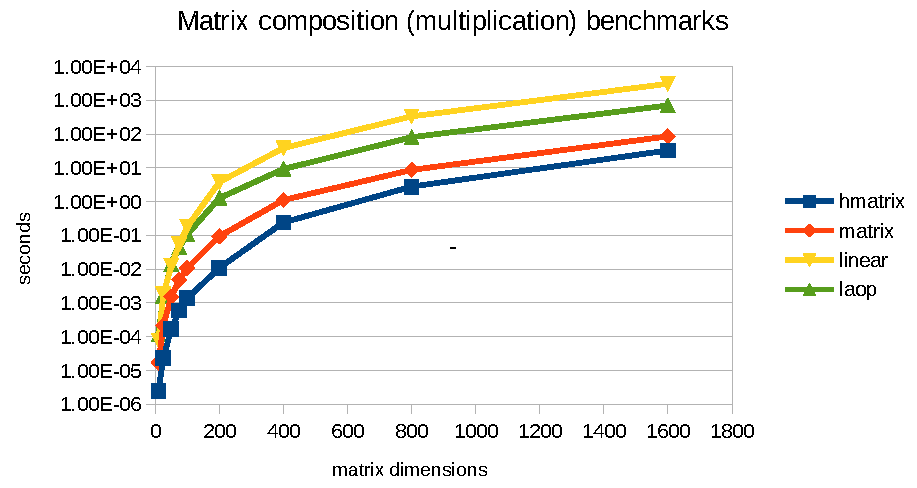
\includegraphics[width=\linewidth]{img/report1.pdf}
        \caption{Matrix composition benchmarks}
        \label{fig:bench}
    \end{figure}
    
    As can be seen in the plot of Figure \ref{fig:bench}, the \emph{hmatrix} and \emph{matrix} libraries are those that perform better. By observing their internal structure, one realises that they are a suitable representation for BLAS/LAPACK computations \citep{anderson1999lapack}, that is, they have been designed to efficiently exploit caches on modern cache-based architectures. A matrix in the \emph{linear} library is defined as \texttt{Vector cols (Vector rows Double)} and does not take into account cache lengths or sizes, so it behaves much worse than the previous ones. Our data structure does not take into account any low-level optimisations either, being unable to compete with those that do. Nevertheless, the implementation is \emph{performant for a cache-oblivious approach} and behaves better (almost one order of magnitude better) than other data types with simpler definitions.
        
        \subsection{Distribution matrix versus distribution list monad}
        
        The previous evaluation focused only on the performance of the proposed matrix multiplication algorithm compared with existing solutions to linear algebra. In this section the use of matrices versus the use of lists as representations of probability distributions will be evaluated, by comparing the performance of the different versions of the \texttt{select} operator. Since both are exhaustive approaches to probabilistic programming, the comparisons will feature the strict applicative version of the \texttt{select} operator (where no computations are skipped) and the more efficient version, which will be called the non-strict version of select, that skips unnecessary computations, to see which solution performs best.
        
        The figure below show the results output by the Criterion framework. The benchmarks have been carried out in the same settings as the previous ones, that is, all matrices and lists were randomly generated.
        
            \begin{figure}[H]%[9]{r}{18em}
            \centering
             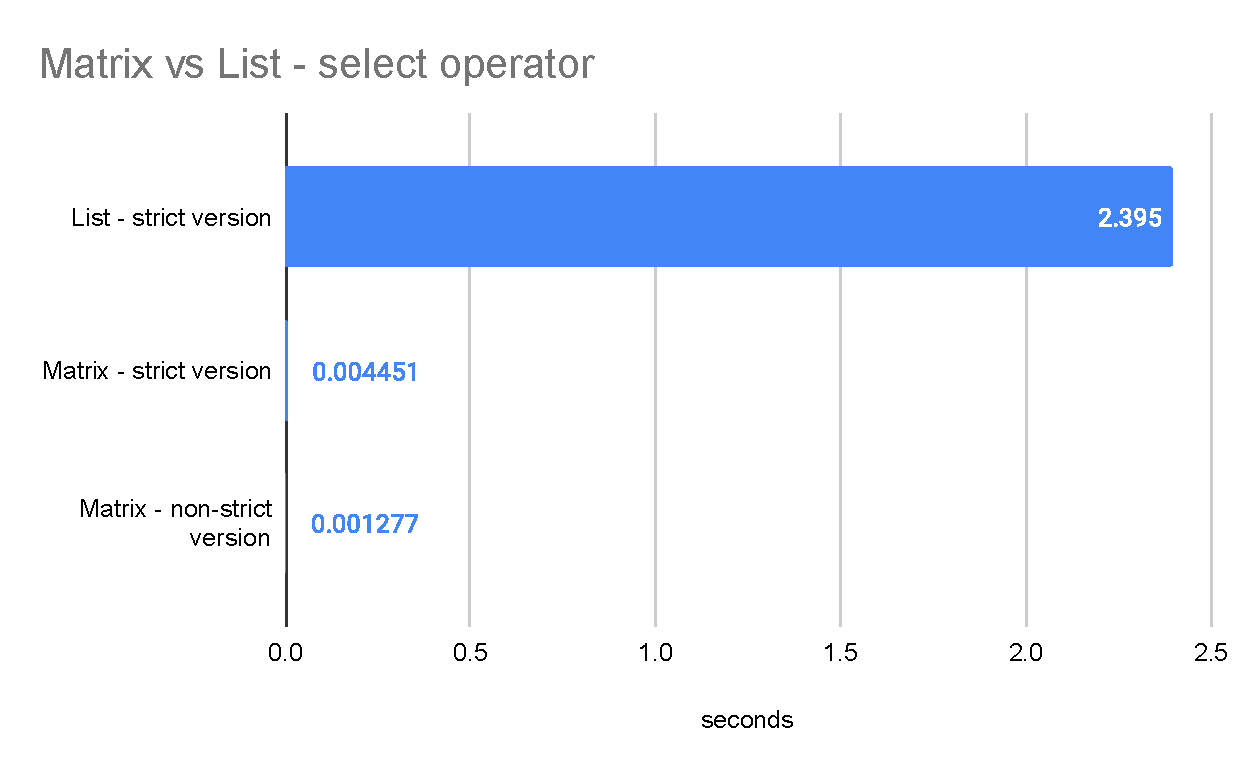
\includegraphics[width=\linewidth]{img/chart.pdf}
               \caption{Matrix vs List - \texttt{select} operator}
               \label{fig:bench2}
            \end{figure}
            
        The first entry, which corresponds to the distribution monad presented by \cite{erwig_kollmansberger_2006} can be seen to perform worse than the others. The strict version of the \texttt{select} operator, in the matrix version, performs better even though no computation is skipped. The last entry, which refers to the non-strict version of the \texttt{select} operator, is also clearly better than its strict version.
        
        There are several attempts that build on the work of \cite{erwig_kollmansberger_2006}, in order to improve the performance of the exhaustive probability monad \citep{larsen2011memory, dylus2018probabilistic}. Allied with the \gls{laop} discipline, the typed, inductive matrix data structure offers a more performant, correct alternative at the cost of a minimum cognitive overhead.
        
    \subsection{Sequential vs Concurrent Selective eDSL}
        This section evaluates the performance of each \gls{edsl} solution provided in sections \ref{prob-edsl} and \ref{prob-conc}. In order to do so, three probabilistic programs were used: one that throws two hypothetical $50000$-faced dice, returning both results; one that throws the same two dice but conditioned the result; and one similar to \texttt{diceThrow} in Listing \ref{lst:dicethrow} but using the same dice as in the previous programs. 
        
        \begin{lstlisting}[language=Haskell, caption={Programs used in evaluation}, captionpos=b]
bigDie :: Dist Int
bigDie = uniform [0 .. 50000]

-- Normal without conditioning
pg1 :: Dist (Int, Int)
pg1 =
  let c1 = bigDie
      c2 = bigDie
   in (,) <$> c1 <*> c2

-- With conditioning
pg2 :: Dist (Maybe (Int, Int))
pg2 =
  let c1 = bigDie
      c2 = bigDie
      result = (,) <$> c1 <*> c2
   in condition (uncurry (>)) result

-- Takes advantage of speculative and parallel execution
pg3 :: Dist Int
pg3 =
  condS
    (pure $ uncurry (==))
    ((\c (a, b) -> a + b + c) <$> die) -- Speculative dice throw
    (pure (\(a, _) -> a + a + a))
    ((,) <$> bigDie <*> bigDie) -- Parallel dice throw
        \end{lstlisting}{}
        
    Each benchmark consists of performing forward sampling $10000$ times, leading to three sets of three benchmarks each. The first collection relates to \texttt{pg1}, the second to \texttt{pg2} and the third to \texttt{pg3}. For each collection, the first benchmark interprets the \gls{edsl} to \texttt{IO} and runs computations sequentially; the second first interprets to the concurrency monad and then \texttt{IO}, running sequentially as well; finally, the third is as the previous one but takes advantage of the concurrent runtime system of \gls{ghc}.
    
    \begin{figure}[H]
        \centering
        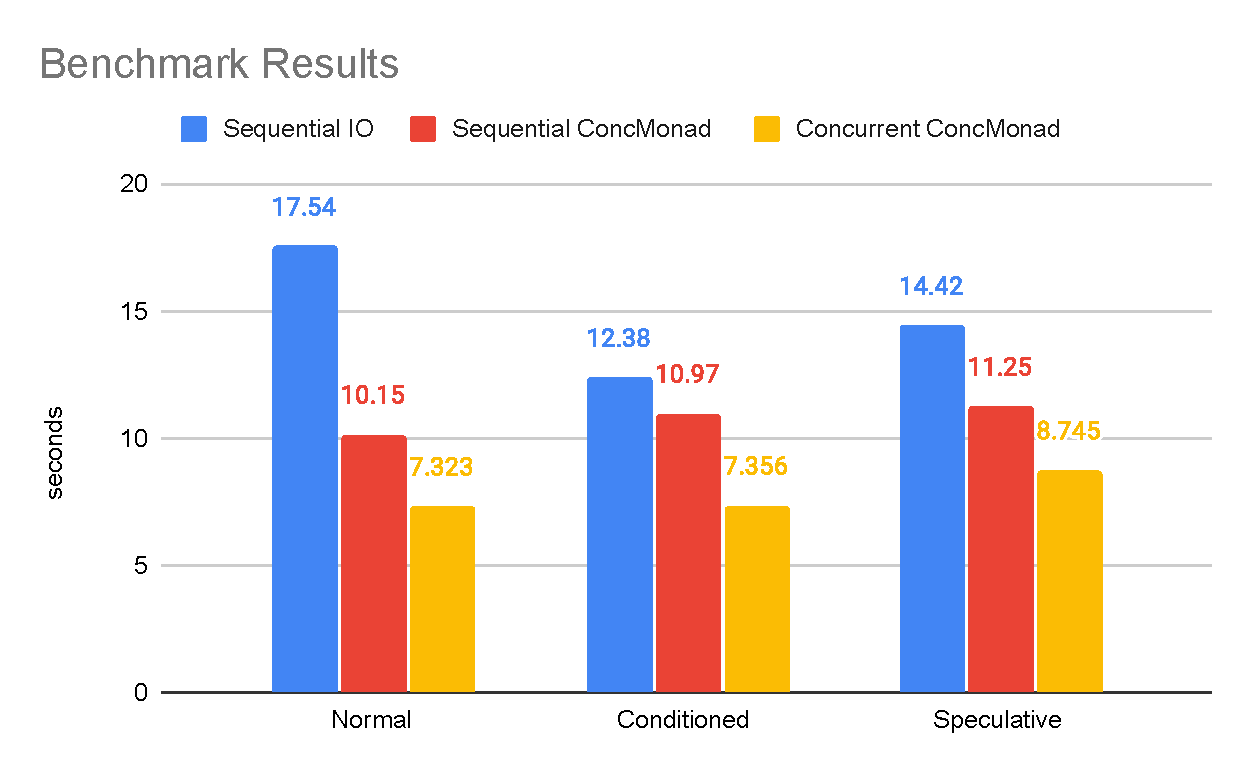
\includegraphics[width=\linewidth]{img/BenchmarkResults.pdf}
        \caption{Benchmarks results}
        \label{fig:no-delay}
    \end{figure}
    
   % From the graph, one can see that there are three distinct sets of benchmarks corresponding to the mentioned above, respectively.
    
    By comparing the blue and red bars of the chart one sees a positive impact on performance, just by switching from pure \texttt{IO} to the concurrency monad. Although the speedup is not as much as doing the first switch, enabling \gls{ghc}'s concurrent runtime system also performs better. The normal variation shown seems to be the one that benefits the most from the optimisations. This fact might be due to the batching ability of independent sampling computations, allowed by the concurrency monad. Since \texttt{pg1} only takes advantage of applicative capabilities, it makes sense that batching is the optimisation with higher influence on the results.
    
    Both the conditioned and the speculative versions make use of selective combinators, such as \texttt{condition} and \texttt{condS}, and thus can take advantage of speculative execution as well. Although these last two benchmarks do not present speedups as significant as the normal version (hinting that batching does not have such an impact), changing to a concurrent runtime system seems to magnify the effect that both, batching and speculative execution, have in the overall performance of the probabilistic sampling.
    
    Looking at the benchmark, sampling from a random distribution such as \texttt{uniform 50000} can be seen as fast. Thus, even without a large sampling gap between the sequential and the concurrent versions, this solution would prove to be a scalable, easy approach to performing such computations in practice. For example, many big data and data mining applications depend on slow uniform data sampling from external sources that require heavy roundtrip times \citep{7917368, kim2019sampling, ZHOU2017350, 10.1145/3203217.3205863}.
    
    \section{Summary}
    
    This chapter described how probabilistic problems can be modelled in the various approaches proposed in the previous chapters. The sprinkler example illustrated the advantages and drawbacks of each of them, touching on the key points of view of the overall design.

    The matrix library was benchmarked with respect to the matrix composition operation, chosen because it is one of the key operations in linear algebra. Given that matrices have an exhaustive approach to the representation of probability distributions, it made sense to compare the proposed solution with the probabilistic monad of \cite{erwig_kollmansberger_2006} and to quantify the impact that the previous study of the \gls{saf} abstraction had in the development of a more efficient implementation of the \texttt{select} operator. Last but not least, the probabilistic programming \gls{edsl} via selective combinators was evaluated. Various types of programs based on different features have been compared with different interpretations (\texttt{IO} or concurrency monad).

    The results achieved can be regarded as satisfactory. On the one hand, the exhaustive matrix approach provides a good trade-off between cognitive overhead and efficiency, rewarding the additional effort needed with guarantees of correctness and assisted reasoning; on the other hand, the use of an \gls{edsl} solves the limitations imposed by the exhaustive approach, and allows for a more idiomatic and richer programming style, from the point of view of the ecosystem of the host language.
    
	% CHAPTER - Conclusion/Future Work --------------
	\chapter{Conclusions and Future Work}\label{ch-conclusion}
	    This last chapter summarises the main  contributions of the dissertation. Directions for future work are also discussed.
	
	   \section{Conclusions}
	   The work reported in this dissertation searched for ways to take advantages of \glspl{saf} in functional probabilistic programming. In particular, how this abstraction could be applied in a more efficient manner than the monadic \texttt{bind} was a central research question. First of all, it was important to understand the meaning of the probabilistic instances of such functors and what they could bring to the table, taking into account other existing solutions and methods.
	        % exist, and their drawbacks. 
	        We centered on the general theory of \gls{laop} when searching for answers to the probabilistic meaning, and studied the structure of stochastic matrices, finding out that \glspl{saf} are capable of conditioning random variables and branching a program in two different ways. Viewed through this prism, \glspl{saf} generalise the already known McCarthy conditional and, in theory, allow for parallel execution of conditional probability calculations, by means of the divide-and-conquer block-matrix algebra law. A programming library of typed inductive block-matrices has been implemented in Haskell to demonstrate how such research could be applied in practice, by giving a number of examples and benchmarks demonstrating that the theoretical gains are indeed valid. 
	        
	        Nevertheless, the use of matrices in probabilistic programming presents some drawbacks regarding programs whose sample space has an explosion of potential states. Sampling from the probability distributions is an alternative in such cases. It turns out that existing solutions rely heavily on the use of monads, which are inherently sequential and, as such, leave behind any possibility of parallel sampling wherever possible. In order to solve this problem, a small probabilistic programming \gls{edsl} was designed on top of the free \gls{saf} construction.
	        
	        In the proposed approach, the end-user is pushed to use selective combinators wherever possible, so that the compiler can be sure to take advantage of the capabilities of this abstraction. The crucial insight in this respect is to realise that the problem of sampling can be reduced to a concurrent external data access problem. Knowing this, it was possible to implement a solution close to that of the Haxl system and use it in the implemented \gls{edsl}. On performance grounds, the outcome was positive compared to the previous sequential version.
	        
	        Altogether, the final conclusion is that, thanks to the nature of \glspl{saf}, one can indeed take advantage of static analysis and speculative execution to write the \texttt{select} operator more efficiently than using, the more traditional, monadic \texttt{bind}.
	        
	    \section{Future work}
	    
	     The work presented in this dissertation highlights the themes of composition, abstraction and structure, all relevant concepts in functional programming. The majority of features developed during this research are focused on core aspects of statically typed, purely functional languages. Monads, definitely a key driver of innovation, cannot be faithfully expressed without a strong type system and functional purity. As we have seen these features have enabled us to have a great deal of reasoning power and have helped us to study novel abstractions in a different (probabilistic) context.
	    
	    All research projects typically have a proof-of-concept feel about them; they are meant to explore new fields, design spaces and opportunities. Specifically for this project, quadtrees \citep{samet1984quadtree} and their savings with respect to repetitive cells (pixels) were brought to mind by the block-oriented matrix type, from the typed matrix programming library. But this can be improved. For instance, a better matrix definition for sparsity could be more useful for sparse matrices with large zero blocks. 
	    
	    A strong suggestion for future work is to turn the various pieces of software that have been developed during this research into production-ready software artifacts.
	    
	    The probabilistic programming \gls{edsl} can also be extended in order to support more distribution primitives and sampling algorithms. An interesting direction for the future is also to investigate how to improve the proposed solution in the light of the new found concurrency relationship, as well as studying parallelization strategies to improve performance. 
	     
	    The work regarding the matrix programming library led to a scientific paper published in the Haskell 2020 Symposium \citep{Armando2020}. This paper attracted the attention of 
	    %some scholars in the fields of computer science, mathematics and functional programming. In particular, 
	    two independent researchers, Conal Elliot and João Paixão, who approached the authors showing interest in potential collaboration. These collaborations point towards new future work directions.
	    %, that also meet the researcher's objectives.
	    
	    In particular, Conal Elliot's work on applying semantic elegance and rigor to library design and optimized implementation led to his interest in investigating how, by applying the denotational design technique to the structure of inductive matrices, one can better understand the nature of linear algebra and find elegant, parallel, effective and correct algorithms. A concrete objective is to port something like the (inductive) matrix type to a purely functional programming language in a denotational design style. To this end, the Haskell programming language is being used to implement all the vocabulary and infrastructure required to start thinking about the problem, but due to the current limitations of the type system, the project is slowly being rewritten in Agda\footnote{The Haskell project: \href{https://github.com/conal/linalg}{https://github.com/conal/linalg}}.
	    
	    João Paixão is a professor of the Department of Computer Science at the Federal University of Rio de Janeiro and his work focuses on Linear Algebra and Numerical Methods Education, Graph Theory, String Diagrams and Graphic Linear Algebra. His work plan is to see if his Graphical Linear Algebra (GLA) language \citep{paixao2020calculational} is capable of expressing inductive matrices taking advantage of its correct-by-construction properties, in order to obtain easy and elegant proof of complex, classical linear algebra algorithms and axioms.
	     
	\bookmarksetup{startatroot} % Ends last part.
	\addtocontents{toc}{\bigskip} % Making the table of contents look good.
	%\cleardoublepage

	%- Bibliography (needs bibtex) -%
	\bibliography{dissertation}

	% Index of terms (needs  makeindex) -------------
	%\printindex
	
	
	% APPENDIX --------------------------------------
	\umappendix{Appendix}
	
	% Add appendix chapters
	\chapter{Type safe LAoP matrix wrapper library}\label{appendix-a}
	
    \begin{lstlisting}[language=Haskell, caption={Type safe matrix wrapper library},captionpos=b]
{-# LANGUAGE AllowAmbiguousTypes #-}
{-# LANGUAGE ConstraintKinds #-}
{-# LANGUAGE DataKinds #-}
{-# LANGUAGE FlexibleContexts #-}
{-# LANGUAGE FlexibleInstances #-}
{-# LANGUAGE GADTs #-}
{-# LANGUAGE GeneralizedNewtypeDeriving #-}
{-# LANGUAGE InstanceSigs #-}
{-# LANGUAGE KindSignatures #-}
{-# LANGUAGE MultiParamTypeClasses #-}
{-# LANGUAGE NoStarIsType #-}
{-# LANGUAGE ScopedTypeVariables #-}
{-# LANGUAGE StandaloneDeriving #-}
{-# LANGUAGE TypeApplications #-}
{-# LANGUAGE TypeOperators #-}
{-# LANGUAGE UndecidableInstances #-}
{-# OPTIONS_GHC -fplugin GHC.TypeLits.KnownNat.Solver #-}

module Matrix.Internal
  ( Matrix (..),
    NonZero,
    ValidDimensions,
    KnownDimensions,
    fromLists,
    toLists,
    toList,
    columns,
    rows,
    matrix,
    tr,
    row,
    col,
    fmapRows,
    fmapColumns,
    ident,
    zeros,
    ones,
    bang,
    diag,
    (|||),
    (===),
    i1,
    i2,
    p1,
    p2,
    (-|-),
    (><),
    kp1,
    kp2,
    khatri,
    selectM,
    comp,
    fromF,
  )
where

import Control.DeepSeq
import Data.Binary
import qualified Data.List as L
import Data.Proxy
import Foreign.Storable
import GHC.TypeLits
import qualified Numeric.LinearAlgebra as LA
import qualified Numeric.LinearAlgebra.Data as HM

-- | The 'Matrix' type is a type safe wrapper around the
-- 'Numeric.LinearAlgebra.Data.Matrix' data type.
newtype Matrix e (c :: Nat) (r :: Nat) = M {unMatrix :: HM.Matrix e}

deriving instance (LA.Container HM.Matrix e) => Eq (Matrix e c r)

deriving instance (LA.Container HM.Vector e, Fractional e, Fractional (HM.Vector e), Num (HM.Matrix e)) => Fractional (Matrix e c r)

deriving instance (Floating e, LA.Container HM.Vector e, Floating (HM.Vector e), Fractional (HM.Matrix e)) => Floating (Matrix e c r)

deriving instance (LA.Container HM.Matrix e, Num e, Num (HM.Vector e)) => Num (Matrix e c r)

deriving instance (Read e, LA.Element e) => Read (Matrix e c r)

deriving instance (Binary (HM.Vector e), LA.Element e) => Binary (Matrix e c r)

deriving instance (Storable e, NFData e) => NFData (Matrix e c r)

instance (Show e, LA.Element e) => Show (Matrix e c r) where
  show (M m) = show m

type NonZero (n :: Nat) = (CmpNat n 0 ~ 'GT)

type ValidDimensions (n :: Nat) (m :: Nat) = (NonZero n, NonZero m)

type KnownDimensions (n :: Nat) (m :: Nat) = (KnownNat n, KnownNat m)

-------------------------------------------------------------------------------
--    CONVERTER FUNCTIONS
-------------------------------------------------------------------------------

-- | Matrix converter function. It builds a matrix from
-- a list of lists @[[e]]@ (considered as rows).
fromLists :: forall e c r. (LA.Element e, KnownDimensions c r) => [[e]] -> Matrix e c r
fromLists [] = error "Wrong list dimensions"
fromLists l@(h : _) =
  let ccols = fromInteger $ natVal (Proxy :: Proxy c)
      rrows = fromInteger $ natVal (Proxy :: Proxy r)
      lrows = length l
      lcols = length h
   in if rrows /= lrows || ccols /= lcols
        then error "Wrong list dimensions"
        else M . HM.fromLists $ l

-- | Matrix converter function. It builds a list of lists from
-- a 'Matrix'.
--
-- Inverse of 'fromLists'.
toLists :: (LA.Element e) => Matrix e c r -> [[e]]
toLists = HM.toLists . unMatrix

-- | Matrix converter function. It builds a list of elements from
-- a 'Matrix'.
toList :: (LA.Element e) => Matrix e c r -> [e]
toList = concat . toLists

-- | Matrix converter function. It builds a matrix from a function.
fromF :: forall c r a b e. (Enum a, Enum b, Eq b, Num e, Ord e, LA.Element e, KnownNat c, KnownNat r) => (a -> b) -> Matrix e c r
fromF f =
  let ccols = fromInteger $ natVal (Proxy :: Proxy c)
      rrows = fromInteger $ natVal (Proxy :: Proxy r)
      elementsA = take ccols $ map toEnum [0 ..]
      elementsB = take rrows $ map toEnum [0 ..]
      combinations = (,) <$> elementsA <*> elementsB
      combAp = map snd . L.sort . map (\(a, b) -> if f a == b then ((fromEnum a, fromEnum b), 1) else ((fromEnum a, fromEnum b), 0)) $ combinations
      mList = buildList combAp rrows
   in tr $ fromLists mList
  where
    buildList [] _ = []
    buildList l r = take r l : buildList (drop r l) r

-------------------------------------------------------------------------------
--    DIMENSIONS FUNCTIONS
-------------------------------------------------------------------------------

-- | Obtain the number of columns of a matrix
columns :: forall e c r. KnownNat c => Matrix e c r -> Integer
columns _ = natVal (Proxy :: Proxy c)

-- | Obtain the number of rows of a matrix
rows :: forall e c r. KnownNat r => Matrix e c r -> Integer
rows _ = natVal (Proxy :: Proxy r)

fmapColumns :: forall b e a r. (Storable e, LA.Element e, KnownNat b) => Matrix e a r -> Matrix e b r
fmapColumns =
  let cols = fromInteger $ natVal (Proxy :: Proxy b)
   in M . HM.reshape cols . HM.fromList . toList

fmapRows :: forall b e a c. (Storable e, LA.Element e, KnownDimensions c b) => Matrix e c a -> Matrix e c b
fmapRows =
  let rows = fromInteger $ natVal (Proxy :: Proxy b)
   in tr . M . HM.reshape rows . HM.fromList . toList

-------------------------------------------------------------------------------
--    MISC FUNCTIONS
-------------------------------------------------------------------------------

-- | Create a matrix.
matrix :: forall e c r. (KnownDimensions c r, Storable e) => [e] -> Matrix e c r
matrix l =
  let m = (reshape @e @c) . HM.fromList $ l
      mcols = HM.cols (unMatrix m)
      mrows = HM.rows (unMatrix m)
      ccols = fromInteger $ natVal (Proxy :: Proxy c)
      rrows = fromInteger $ natVal (Proxy :: Proxy r)
   in if mcols /= ccols || mrows /= rrows
        then error "Wrong list dimensions"
        else m

-- | Matrix transpose
tr :: forall e c r. (LA.Element e, KnownDimensions c r) => Matrix e c r -> Matrix e r c
tr = fromLists . L.transpose . toLists

-- | Create a row vector matrix.
row :: (Storable e, LA.Element e, KnownNat c) => [e] -> Matrix e c 1
row = asRow . HM.fromList

-- | Create a column vector matrix.
col :: (Storable e) => [e] -> Matrix e 1 r
col = asColumn . HM.fromList

-- | Creates the identity matrix of given dimension.
ident :: forall e c. (Num e, LA.Element e, KnownNat c) => Matrix e c c
ident =
  let c = fromInteger $ natVal (Proxy :: Proxy c)
   in M . HM.ident $ c

-- | Zero Matrix polymorphic definition
zeros :: forall e c r. (KnownDimensions c r, Num e, LA.Container HM.Vector e) => Matrix e c r
zeros =
  let ccols = fromInteger $ natVal (Proxy :: Proxy c)
      rrows = fromInteger $ natVal (Proxy :: Proxy r)
   in M $ HM.konst 0 (rrows, ccols)

-- | One Matrix polymorphic definition
ones :: forall e c r. (KnownDimensions c r, Num e, LA.Container HM.Vector e) => Matrix e c r
ones =
  let ccols = fromInteger $ natVal (Proxy :: Proxy c)
      rrows = fromInteger $ natVal (Proxy :: Proxy r)
   in M $ HM.konst 1 (rrows, ccols)

-- | Bang Matrix polymorphic Matrix
bang :: forall e c . (KnownNat c, Num e, LA.Container HM.Vector e) => Matrix e c 1
bang =
  let ccols = fromInteger $ natVal (Proxy :: Proxy c)
   in M $ HM.konst 1 (1, ccols)

-- | Creates a square matrix with a given diagonal.
diag :: forall e c. (Num e, LA.Element e, KnownNat c) => [e] -> Matrix e c c
diag l =
  let c = fromInteger $ natVal (Proxy :: Proxy c)
      dims = length l
   in if c /= dims
        then error "Wrong list dimensions"
        else M . HM.diag . HM.fromList $ l

-------------------------------------------------------------------------------
--    BLOCK MATRIX FUNCTIONS (BIPRODUCT)
-------------------------------------------------------------------------------

-- | Matrix block algebra 'Junc' operator
(|||) :: (LA.Element e, ValidDimensions n m, NonZero p) => Matrix e m p -> Matrix e n p -> Matrix e (m + n) p
(|||) a b = M $ HM.fromBlocks [[unMatrix a, unMatrix b]]

infixl 3 |||

-- | Matrix block algebra 'Split' operator
(===) :: (LA.Element e, ValidDimensions n m, NonZero p) => Matrix e p m -> Matrix e p n -> Matrix e p (m + n)
(===) a b = M $ HM.fromBlocks [[unMatrix a], [unMatrix b]]

infixl 2 ===

-- | Matrix 'Junc' left injection matrix definition
i1 :: (Num e, ValidDimensions n m, KnownDimensions n m, LA.Element e, LA.Container HM.Vector e) => Matrix e m (m + n)
i1 = ident === zeros

-- | Matrix 'Junc' right injection matrix definition
i2 :: (Num e, ValidDimensions n m, KnownDimensions n m, LA.Element e, LA.Container HM.Vector e) => Matrix e n (m + n)
i2 = zeros === ident

-- | Matrix 'Split' left projection matrix definition
p1 :: (Num e, ValidDimensions n m, KnownDimensions n m, KnownNat (m + n), LA.Element e, LA.Container HM.Vector e) => Matrix e (m + n) m
p1 = tr i1

-- | Matrix 'Split' right projection matrix definition
p2 :: (Num e, ValidDimensions n m, KnownDimensions n m, KnownNat (m + n), LA.Element e, LA.Container HM.Vector e) => Matrix e (m + n) n
p2 = tr i2

-------------------------------------------------------------------------------
--    MATRIX BIPRODUCT FUNCTORS
-------------------------------------------------------------------------------

-- | Matrix coproduct bifunctor
(-|-) ::
  forall e n m j k.
  ( ValidDimensions n m,
    ValidDimensions k j,
    NonZero (k + j),
    LA.Element e,
    LA.Numeric e,
    KnownDimensions k j
  ) =>
  Matrix e n k ->
  Matrix e m j ->
  Matrix e (n + m) (k + j)
(-|-) a b = (i1 `comp` a) ||| (i2 `comp` b)

infixl 5 -|-

-- | Kronecker product of two matrices
(><) :: LA.Product e => Matrix e m p -> Matrix e n q -> Matrix e (m * n) (p * q)
(><) (M a) (M b) = M . LA.kronecker a $ b

infixl 4 ><

-------------------------------------------------------------------------------
--    MATRIX SELECTVIE EQUIVALENT FUNCTION
-------------------------------------------------------------------------------

selectM ::
  ( LA.Numeric e,
    Enum a,
    Enum b,
    Ord e,
    Eq b,
    KnownDimensions m1 m2,
    ValidDimensions m1 m2
  ) =>
  Matrix e n (m1 + m2) -> (a -> b) -> Matrix e n m2
selectM m y = (fromF y ||| ident) `comp` m

-------------------------------------------------------------------------------
--    MATRIX COMPOSITION, KHATRI RAO FUNCTIONS
-------------------------------------------------------------------------------

-- | Matrix - Matrix multiplication aka Matrix composition
comp :: LA.Numeric e => Matrix e p m -> Matrix e n p -> Matrix e n m
comp (M a) (M b) = M . (LA.<>) a $ b

-- | Khatri Rao product left projection (inductive definition)
class KhatriP1 e (m :: Nat) (k :: Nat) where
  kp1 :: Matrix e (m * k) m

instance
  {-# OVERLAPPING #-}
  ( KnownNat k,
    Num e,
    LA.Numeric e,
    LA.Container HM.Vector e
  ) =>
  KhatriP1 e 1 k
  where
  kp1 = ones @e @k @1

instance
  {-# OVERLAPPABLE #-}
  ( ValidDimensions m k,
    KnownNat k,
    KnownNat ((m - 1) * k),
    KnownNat (m - 1),
    Num e,
    LA.Numeric e,
    LA.Container HM.Vector e,
    (1 + (m - 1)) ~ m,
    (k + ((m - 1) * k)) ~ (m * k),
    NonZero ((m - 1) * k),
    NonZero (m - 1),
    KhatriP1 e (m - 1) k
  ) =>
  KhatriP1 e m k
  where
  kp1 = ones @e @k @1 -|- kp1 @e @(m - 1) @k

-- | Khatri Rao product right projection (inductive definition)
class KhatriP2 e (k :: Nat) (m :: Nat) where
  kp2 :: Matrix e (m * k) k

instance
  {-# OVERLAPPING #-}
  ( Num e,
    LA.Element e,
    KnownNat k
  ) =>
  KhatriP2 e k 1
  where
  kp2 = ident @e @k

instance
  {-# OVERLAPPABLE #-}
  ( (k + ((m - 1) * k)) ~ (m * k),
    ValidDimensions m k,
    NonZero ((m - 1) * k),
    LA.Element e,
    Num e,
    KnownNat k,
    KhatriP2 e k (m - 1)
  ) =>
  KhatriP2 e k m
  where
  kp2 = ident @e @k ||| kp2 @e @k @(m - 1)

-- | Khatri Rao product of two matrices (Pairing)
khatri ::
  forall e m p q.
  ( KnownDimensions p (p * q),
    KnownNat q,
    Num e,
    Num (HM.Vector e),
    LA.Numeric e,
    LA.Container HM.Vector e,
    KhatriP1 e p q,
    KhatriP2 e q p
  ) =>
  Matrix e m p ->
  Matrix e m q ->
  Matrix e m (p * q)
khatri a b = (tr (kp1 @e @p @q) `comp` a) * (tr (kp2 @e @q @p) `comp` b)

-------------------------------------------------------------------------------
--    AUXILIARY FUNCTIONS
-------------------------------------------------------------------------------

-- | Creates a matrix from a vector by grouping the elements in rows
-- with the desired number of columns.
reshape :: forall e c r. (Storable e, KnownNat c) => HM.Vector e -> Matrix e c r
reshape v =
  let cols = fromInteger $ natVal (Proxy :: Proxy c)
   in M $ HM.reshape cols v

-- | Creates a 1-column matrix from a vector.
asColumn :: forall e r. (Storable e) => HM.Vector e -> Matrix e 1 r
asColumn = reshape @e @1

-- | Creates a 1-vector matrix from a vector.
asRow :: (Storable e, LA.Element e, KnownNat c) => HM.Vector e -> Matrix e c 1
asRow = tr . asColumn
    \end{lstlisting}
    
	\chapter{Type safe LAoP inductive matrix definition library}\label{appendix-b}
	
    \begin{lstlisting}[language=Haskell, caption={Type safe inductive matrix library},captionpos=b]
{-# LANGUAGE AllowAmbiguousTypes #-}
{-# LANGUAGE DataKinds #-}
{-# LANGUAGE FlexibleContexts #-}
{-# LANGUAGE FlexibleInstances #-}
{-# LANGUAGE GADTs #-}
{-# LANGUAGE InstanceSigs #-}
{-# LANGUAGE MultiParamTypeClasses #-}
{-# LANGUAGE NoStarIsType #-}
{-# LANGUAGE ScopedTypeVariables #-}
{-# LANGUAGE StandaloneDeriving #-}
{-# LANGUAGE TypeApplications #-}
{-# LANGUAGE TypeFamilies #-}
{-# LANGUAGE TypeOperators #-}
{-# LANGUAGE UndecidableInstances #-}

-----------------------------------------------------------------------------
-- |
-- Module     : Matrix.Internal
-- Copyright  : (c) Armando Santos 2019-2020
-- Maintainer : armandoifsantos@gmail.com
-- Stability  : experimental
--
-- The LAoP discipline generalises relations and functions treating them as
-- Boolean matrices and in turn consider these as arrows.
--
-- __LAoP__ is a library for algebraic (inductive) construction and manipulation of matrices
-- in Haskell. See <https://github.com/bolt12/master-thesis my Msc Thesis> for the
-- motivation behind the library, the underlying theory, and implementation details.
--
-- This module offers many of the combinators mentioned in the work of
-- Macedo (2012) and Oliveira (2012). 
--
-- This is an Internal module and it is no supposed to be imported.
--
-----------------------------------------------------------------------------

module Matrix.Internal
  ( -- | This definition makes use of the fact that 'Void' is
    -- isomorphic to 0 and '()' to 1 and captures matrix
    -- dimensions as stacks of 'Either's.
    --
    -- There exists two type families that make it easier to write
    -- matrix dimensions: 'FromNat' and 'Count'. This approach
    -- leads to a very straightforward implementation 
    -- of LAoP combinators. 

    -- * Type safe matrix representation
    Matrix (..),

    -- * Primitives
    empty,
    one,
    junc,
    split,

    -- * Auxiliary type families
    FromNat,
    Count,
    Normalize,

    -- * Matrix construction and conversion
    FromLists,
    fromLists,
    toLists,
    toList,
    matrixBuilder,
    row,
    col,
    zeros,
    ones,
    bang,
    constant,

    -- * Misc
    -- ** Get dimensions
    columns,
    rows,

    -- ** Matrix Transposition
    tr,

    -- ** Selective operator
    select, 

    -- ** McCarthy's Conditional
    cond,

    -- ** Matrix "abiding"
    abideJS,
    abideSJ,

    -- * Biproduct approach
    -- ** Split
    (===),
    -- *** Projections
    p1,
    p2,
    -- ** Junc
    (|||),
    -- *** Injections
    i1,
    i2,
    -- ** Bifunctors
    (-|-),
    (><),

    -- ** Applicative matrix combinators

    -- | Note that given the restrictions imposed it is not possible to
    -- implement the standard type classes present in standard Haskell.
    -- *** Matrix pairing projections
    kp1,
    kp2,

    -- *** Matrix pairing
    khatri,

    -- * Matrix composition and lifting

    -- ** Arrow matrix combinators

    -- | Note that given the restrictions imposed it is not possible to
    -- implement the standard type classes present in standard Haskell.
    identity,
    comp,
    fromF,
    fromF',

    -- * Matrix printing
    pretty,
    prettyPrint
  )
    where

import Utils
import Data.Bool
import Data.Kind
import Data.List
import Data.Proxy
import Data.Void
import GHC.TypeLits
import Data.Type.Equality
import GHC.Generics
import Control.DeepSeq
import Control.Category
import Prelude hiding ((.))

-- | LAoP (Linear Algebra of Programming) Inductive Matrix definition.
data Matrix e cols rows where
  Empty :: Matrix e Void Void
  One :: e -> Matrix e () ()
  Junc :: Matrix e a rows -> Matrix e b rows -> Matrix e (Either a b) rows
  Split :: Matrix e cols a -> Matrix e cols b -> Matrix e cols (Either a b)

deriving instance (Show e) => Show (Matrix e cols rows)

-- | Type family that computes the cardinality of a given type dimension.
--
--   It can also count the cardinality of custom types that implement the
-- 'Generic' instance.
type family Count (d :: Type) :: Nat where
  Count (Natural n m) = (m - n) + 1
  Count (Either a b) = (+) (Count a) (Count b)
  Count (a, b) = (*) (Count a) (Count b)
  Count (a -> b) = (^) (Count b) (Count a)
  -- Generics
  Count (M1 _ _ f p) = Count (f p)
  Count (K1 _ _ _) = 1
  Count (V1 _) = 0
  Count (U1 _) = 1
  Count ((:*:) a b p) = Count (a p) * Count (b p)
  Count ((:+:) a b p) = Count (a p) + Count (b p)
  Count d = Count (Rep d R)

-- | Type family that computes of a given type dimension from a given natural
--
--   Thanks to Li-Yao Xia this type family is super fast.
type family FromNat (n :: Nat) :: Type where
  FromNat 0 = Void
  FromNat 1 = ()
  FromNat n = FromNat' (Mod n 2 == 0) (FromNat (Div n 2))

type family FromNat' (b :: Bool) (m :: Type) :: Type where
  FromNat' 'True m = Either m m
  FromNat' 'False m = Either () (Either m m)

-- | Type family that normalizes the representation of a given data
-- structure
type family Normalize (d :: Type) :: Type where
  Normalize d = FromNat (Count d)

-- | It is not possible to implement the 'id' function so it is
-- implementation is 'undefined'. However 'comp' can be and this partial
-- class implementation exists just to make the code more readable.
--
-- Please use 'identity' instead.
instance (Num e) => Category (Matrix e) where
    id = undefined
    (.) = comp

instance NFData e => NFData (Matrix e cols rows) where
    rnf Empty = ()
    rnf (One e) = rnf e
    rnf (Junc a b) = rnf a `seq` rnf b
    rnf (Split a b) = rnf a `seq` rnf b

instance Eq e => Eq (Matrix e cols rows) where
  Empty == Empty                = True
  (One a) == (One b)            = a == b
  (Junc a b) == (Junc c d)      = a == c && b == d
  (Split a b) == (Split c d)    = a == c && b == d
  x@(Split a b) == y@(Junc c d) = x == abideJS y
  x@(Junc a b) == y@(Split c d) = abideJS x == y

instance Num e => Num (Matrix e cols rows) where

  Empty + Empty                = Empty
  (One a) + (One b)            = One (a + b)
  (Junc a b) + (Junc c d)      = Junc (a + c) (b + d)
  (Split a b) + (Split c d)    = Split (a + c) (b + d)
  x@(Split a b) + y@(Junc c d) = x + abideJS y
  x@(Junc a b) + y@(Split c d) = abideJS x + y

  Empty - Empty             = Empty
  (One a) - (One b)         = One (a - b)
  (Junc a b) - (Junc c d)   = Junc (a - c) (b - d)
  (Split a b) - (Split c d) = Split (a - c) (b - d)
  x@(Split a b) - y@(Junc c d) = x - abideJS y
  x@(Junc a b) - y@(Split c d) = abideJS x - y

  Empty * Empty             = Empty
  (One a) * (One b)         = One (a * b)
  (Junc a b) * (Junc c d)   = Junc (a * c) (b * d)
  (Split a b) * (Split c d) = Split (a * c) (b * d)
  x@(Split a b) * y@(Junc c d) = x * abideJS y
  x@(Junc a b) * y@(Split c d) = abideJS x * y

  abs Empty       = Empty
  abs (One a)     = One (abs a)
  abs (Junc a b)  = Junc (abs a) (abs b)
  abs (Split a b) = Split (abs a) (abs b)

  signum Empty       = Empty
  signum (One a)     = One (signum a)
  signum (Junc a b)  = Junc (signum a) (signum b)
  signum (Split a b) = Split (signum a) (signum b)

-- Primitives

-- | Empty matrix constructor
empty :: Matrix e Void Void
empty = Empty

-- | Unit matrix constructor
one :: e -> Matrix e () ()
one = One

-- | Matrix 'Junc' constructor
junc :: Matrix e a rows -> Matrix e b rows -> Matrix e (Either a b) rows
junc = Junc

infixl 3 |||

-- | Matrix 'Junc' constructor
(|||) :: Matrix e a rows -> Matrix e b rows -> Matrix e (Either a b) rows
(|||) = Junc

-- | Matrix 'Split' constructor
split :: Matrix e cols a -> Matrix e cols b -> Matrix e cols (Either a b)
split = Split

infixl 2 ===

-- | Matrix 'Split' constructor
(===) :: Matrix e cols a -> Matrix e cols b -> Matrix e cols (Either a b)
(===) = Split

-- Construction

-- | Type class for defining the 'fromList' conversion function.
--
--   Given that it is not possible to branch on types at the term level type
-- classes are needed bery much like an inductive definition but on types.
class FromLists e cols rows where
  -- | Build a matrix out of a list of list of elements. Throws a runtime
  -- error if the dimensions do not match.
  fromLists :: [[e]] -> Matrix e cols rows

instance FromLists e Void Void where
  fromLists [] = Empty
  fromLists _  = error "Wrong dimensions"

instance {-# OVERLAPPING #-} FromLists e () () where
  fromLists [[e]] = One e
  fromLists _     = error "Wrong dimensions"

instance {-# OVERLAPPING #-} (FromLists e cols ()) => FromLists e (Either () cols) () where
  fromLists [h : t] = Junc (One h) (fromLists [t])
  fromLists _       = error "Wrong dimensions"

instance {-# OVERLAPPABLE #-} (FromLists e a (), FromLists e b (), KnownNat (Count a)) => FromLists e (Either a b) () where
  fromLists [l] = 
      let rowsA = fromInteger (natVal (Proxy :: Proxy (Count a)))
       in Junc (fromLists [take rowsA l]) (fromLists [drop rowsA l])
  fromLists _       = error "Wrong dimensions"

instance {-# OVERLAPPING #-} (FromLists e () rows) => FromLists e () (Either () rows) where
  fromLists ([h] : t) = Split (One h) (fromLists t)
  fromLists _         = error "Wrong dimensions"

instance {-# OVERLAPPABLE #-} (FromLists e () a, FromLists e () b, KnownNat (Count a)) => FromLists e () (Either a b) where
  fromLists l@([h] : t) = 
      let rowsA = fromInteger (natVal (Proxy :: Proxy (Count a)))
       in Split (fromLists (take rowsA l)) (fromLists (drop rowsA l))
  fromLists _         = error "Wrong dimensions"

instance {-# OVERLAPPABLE #-} (FromLists e (Either a b) c, FromLists e (Either a b) d, KnownNat (Count c)) => FromLists e (Either a b) (Either c d) where
  fromLists l@(h : t) =
    let lh        = length h
        rowsC     = fromInteger (natVal (Proxy :: Proxy (Count c)))
        condition = all (== lh) (map length t)
     in if lh > 0 && condition
          then Split (fromLists (take rowsC l)) (fromLists (drop rowsC l))
          else error "Not all rows have the same length"

-- | Matrix builder function. Constructs a matrix provided with
-- a construction function.
matrixBuilder ::
  forall e cols rows.
  ( FromLists e cols rows,
    KnownNat (Count cols),
    KnownNat (Count rows)
  ) =>
  ((Int, Int) -> e) ->
  Matrix e cols rows
matrixBuilder f =
  let c         = fromInteger $ natVal (Proxy :: Proxy (Count cols))
      r         = fromInteger $ natVal (Proxy :: Proxy (Count rows))
      positions = [(a, b) | a <- [0 .. (r - 1)], b <- [0 .. (c - 1)]]
   in fromLists . map (map f) . groupBy (\(x, _) (w, _) -> x == w) $ positions

-- | Constructs a column vector matrix
col :: (FromLists e () rows) => [e] -> Matrix e () rows
col = fromLists . map (: [])

-- | Constructs a row vector matrix
row :: (FromLists e cols ()) => [e] -> Matrix e cols ()
row = fromLists . (: [])

-- | Lifts functions to matrices with arbitrary dimensions.
--
--   NOTE: Be careful to not ask for a matrix bigger than the cardinality of
-- types @a@ or @b@ allows.
fromF ::
  forall a b cols rows e.
  ( Bounded a,
    Bounded b,
    Enum a,
    Enum b,
    Eq b,
    Num e,
    Ord e,
    KnownNat (Count cols),
    KnownNat (Count rows),
    FromLists e rows cols
  ) =>
  (a -> b) ->
  Matrix e cols rows
fromF f =
  let minA         = minBound @a
      maxA         = maxBound @a
      minB         = minBound @b
      maxB         = maxBound @b
      ccols        = fromInteger $ natVal (Proxy :: Proxy (Count cols))
      rrows        = fromInteger $ natVal (Proxy :: Proxy (Count rows))
      elementsA    = take ccols [minA .. maxA]
      elementsB    = take rrows [minB .. maxB]
      combinations = (,) <$> elementsA <*> elementsB
      combAp       = map snd . sort . map (\(a, b) -> if f a == b 
                                                         then ((fromEnum a, fromEnum b), 1) 
                                                         else ((fromEnum a, fromEnum b), 0)) $ combinations
      mList        = buildList combAp rrows
   in tr $ fromLists mList
  where
    buildList [] _ = []
    buildList l r  = take r l : buildList (drop r l) r

-- | Lifts functions to matrices with dimensions matching @a@ and @b@
-- cardinality's.
fromF' ::
  forall a b e.
  ( Bounded a,
    Bounded b,
    Enum a,
    Enum b,
    Eq b,
    Num e,
    Ord e,
    KnownNat (Count (Normalize a)),
    KnownNat (Count (Normalize b)),
    FromLists e (Normalize b) (Normalize a)
  ) =>
  (a -> b) ->
  Matrix e (Normalize a) (Normalize b)
fromF' f =
  let minA         = minBound @a
      maxA         = maxBound @a
      minB         = minBound @b
      maxB         = maxBound @b
      ccols        = fromInteger $ natVal (Proxy :: Proxy (Count (Normalize a)))
      rrows        = fromInteger $ natVal (Proxy :: Proxy (Count (Normalize b)))
      elementsA    = take ccols [minA .. maxA]
      elementsB    = take rrows [minB .. maxB]
      combinations = (,) <$> elementsA <*> elementsB
      combAp       = map snd . sort . map (\(a, b) -> if f a == b 
                                                         then ((fromEnum a, fromEnum b), 1) 
                                                         else ((fromEnum a, fromEnum b), 0)) $ combinations
      mList        = buildList combAp rrows
   in tr $ fromLists mList
  where
    buildList [] _ = []
    buildList l r  = take r l : buildList (drop r l) r

-- Conversion

-- | Converts a matrix to a list of lists of elements.
toLists :: Matrix e cols rows -> [[e]]
toLists Empty       = []
toLists (One e)     = [[e]]
toLists (Split l r) = toLists l ++ toLists r
toLists (Junc l r)  = zipWith (++) (toLists l) (toLists r)

-- | Converts a matrix to a list of elements.
toList :: Matrix e cols rows -> [e]
toList = concat . toLists

-- Zeros Matrix

-- | The zero matrix. A matrix wholly filled with zeros.
zeros :: (Num e, FromLists e cols rows, KnownNat (Count cols), KnownNat (Count rows)) => Matrix e cols rows
zeros = matrixBuilder (const 0)

-- Ones Matrix

-- | The ones matrix. A matrix wholly filled with ones.
--
--   Also known as T (Top) matrix.
ones :: (Num e, FromLists e cols rows, KnownNat (Count cols), KnownNat (Count rows)) => Matrix e cols rows
ones = matrixBuilder (const 1)

-- Const Matrix

-- | The constant matrix constructor. A matrix wholly filled with a given
-- value.
constant :: (Num e, FromLists e cols rows, KnownNat (Count cols), KnownNat (Count rows)) => e -> Matrix e cols rows
constant e = matrixBuilder (const e)

-- Bang Matrix

-- | The T (Top) row vector matrix.
bang :: forall e cols. (Num e, Enum e, FromLists e cols (), KnownNat (Count cols)) => Matrix e cols ()
bang =
  let c = fromInteger $ natVal (Proxy :: Proxy (Count cols))
   in fromLists [take c [1, 1 ..]]

-- Identity Matrix

-- | Identity matrix.
identity :: (Num e, FromLists e cols cols, KnownNat (Count cols)) => Matrix e cols cols
identity = matrixBuilder (bool 0 1 . uncurry (==))

-- Matrix composition (MMM)

-- | Matrix composition. Equivalent to matrix-matrix multiplication.
--
--   This definition takes advantage of divide-and-conquer and fusion laws
-- from LAoP.
comp :: (Num e) => Matrix e cr rows -> Matrix e cols cr -> Matrix e cols rows
comp Empty Empty            = Empty
comp (One a) (One b)        = One (a * b)
comp (Junc a b) (Split c d) = comp a c + comp b d         -- Divide-and-conquer law
comp (Split a b) c          = Split (comp a c) (comp b c) -- Split fusion law
comp c (Junc a b)           = Junc (comp c a) (comp c b)  -- Junc fusion law

-- Projections

-- | Biproduct first component projection
p1 :: forall e m n. (Num e, KnownNat (Count n), KnownNat (Count m), FromLists e n m, FromLists e m m) => Matrix e (Either m n) m
p1 =
  let iden = identity :: Matrix e m m
      zero = zeros :: Matrix e n m
   in junc iden zero

-- | Biproduct second component projection
p2 :: forall e m n. (Num e, KnownNat (Count n), KnownNat (Count m), FromLists e m n, FromLists e n n) => Matrix e (Either m n) n
p2 =
  let iden = identity :: Matrix e n n
      zero = zeros :: Matrix e m n
   in junc zero iden

-- Injections

-- | Biproduct first component injection
i1 :: (Num e, KnownNat (Count n), KnownNat (Count m), FromLists e n m, FromLists e m m) => Matrix e m (Either m n)
i1 = tr p1

-- | Biproduct second component injection
i2 :: (Num e, KnownNat (Count n), KnownNat (Count m), FromLists e m n, FromLists e n n) => Matrix e n (Either m n)
i2 = tr p2

-- Dimensions

-- | Obtain the number of rows.
--
--   NOTE: The 'KnownNat' constaint is needed in order to obtain the
-- dimensions in constant time.
--
-- TODO: A 'rows' function that does not need the 'KnownNat' constraint in
-- exchange for performance.
rows :: forall e cols rows. (KnownNat (Count rows)) => Matrix e cols rows -> Int
rows _ = fromInteger $ natVal (Proxy :: Proxy (Count rows))

-- | Obtain the number of columns.
-- 
--   NOTE: The 'KnownNat' constaint is needed in order to obtain the
-- dimensions in constant time.
--
-- TODO: A 'columns' function that does not need the 'KnownNat' constraint in
-- exchange for performance.
columns :: forall e cols rows. (KnownNat (Count cols)) => Matrix e cols rows -> Int
columns _ = fromInteger $ natVal (Proxy :: Proxy (Count cols))

-- Coproduct Bifunctor

infixl 5 -|-

-- | Matrix coproduct functor also known as matrix direct sum.
(-|-) ::
  forall e n k m j.
  ( Num e,
    KnownNat (Count j),
    KnownNat (Count k),
    FromLists e k k,
    FromLists e j k,
    FromLists e k j,
    FromLists e j j
  ) =>
  Matrix e n k ->
  Matrix e m j ->
  Matrix e (Either n m) (Either k j)
(-|-) a b = Junc (i1 . a) (i2 . b)

-- Khatri Rao Product and projections

-- | Khatri Rao product first component projection matrix.
kp1 :: 
  forall e m k .
  ( Num e,
    KnownNat (Count k),
    FromLists e (FromNat (Count m * Count k)) m,
    KnownNat (Count m),
    KnownNat (Count (Normalize (m, k)))
  ) => Matrix e (Normalize (m, k)) m
kp1 = matrixBuilder f
  where
    offset = fromInteger (natVal (Proxy :: Proxy (Count k)))
    f (x, y)
      | y >= (x * offset) && y <= (x * offset + offset - 1) = 1
      | otherwise = 0

-- | Khatri Rao product second component projection matrix.
kp2 :: 
    forall e m k .
    ( Num e,
      KnownNat (Count k),
      FromLists e (FromNat (Count m * Count k)) k,
      KnownNat (Count m),
      KnownNat (Count (Normalize (m, k)))
    ) => Matrix e (Normalize (m, k)) k
kp2 = matrixBuilder f
  where
    offset = fromInteger (natVal (Proxy :: Proxy (Count k)))
    f (x, y)
      | x == y || mod (y - x) offset == 0 = 1
      | otherwise                         = 0

-- | Khatri Rao Matrix product also known as matrix pairing.
--
--   NOTE: That this is not a true categorical product, see for instance:
-- 
-- @
--                | kp1 . khatri a b == a 
-- khatri a b ==> |
--                | kp2 . khatri a b == b
-- @
--
-- __Emphasis__ on the implication symbol.
khatri :: 
       forall e cols a b. 
       ( Num e,
         KnownNat (Count a),
         KnownNat (Count b),
         KnownNat (Count (Normalize (a, b))),
         FromLists e (Normalize (a, b)) a,
         FromLists e (Normalize (a, b)) b
       ) => Matrix e cols a -> Matrix e cols b -> Matrix e cols (Normalize (a, b))
khatri a b =
  let kp1' = kp1 @e @a @b
      kp2' = kp2 @e @a @b
   in (tr kp1') . a * (tr kp2') . b

-- Product Bifunctor (Kronecker)

infixl 4 ><

-- | Matrix product functor also known as kronecker product
(><) :: 
     forall e m p n q. 
     ( Num e,
       KnownNat (Count m),
       KnownNat (Count n),
       KnownNat (Count p),
       KnownNat (Count q),
       KnownNat (Count (Normalize (m, n))),
       FromLists e (Normalize (m, n)) m,
       FromLists e (Normalize (m, n)) n,
       KnownNat (Count (Normalize (p, q))),
       FromLists e (Normalize (p, q)) p,
       FromLists e (Normalize (p, q)) q
     ) 
     => Matrix e m p -> Matrix e n q -> Matrix e (Normalize (m, n)) (Normalize (p, q))
(><) a b =
  let kp1' = kp1 @e @m @n
      kp2' = kp2 @e @m @n
   in khatri (a . kp1') (b . kp2')

-- Matrix abide Junc Split

-- | Matrix "abiding" followin the 'Junc'-'Split' abide law.
-- 
-- Law:
--
-- @
-- 'Junc' ('Split' a c) ('Split' b d) == 'Split' ('Junc' a b) ('Junc' c d)
-- @
abideJS :: Matrix e cols rows -> Matrix e cols rows
abideJS (Junc (Split a c) (Split b d)) = Split (Junc (abideJS a) (abideJS b)) (Junc (abideJS c) (abideJS d)) -- Junc-Split abide law
abideJS Empty                          = Empty
abideJS (One e)                        = One e
abideJS (Junc a b)                     = Junc (abideJS a) (abideJS b)
abideJS (Split a b)                    = Split (abideJS a) (abideJS b)

-- Matrix abide Split Junc

-- | Matrix "abiding" followin the 'Split'-'Junc' abide law.
-- 
-- @
-- 'Split' ('Junc' a b) ('Junc' c d) == 'Junc' ('Split' a c) ('Split' b d)
-- @
abideSJ :: Matrix e cols rows -> Matrix e cols rows
abideSJ (Split (Junc a b) (Junc c d)) = Junc (Split (abideSJ a) (abideSJ c)) (Split (abideSJ b) (abideSJ d)) -- Split-Junc abide law
abideSJ Empty                         = Empty
abideSJ (One e)                       = One e
abideSJ (Junc a b)                    = Junc (abideSJ a) (abideSJ b)
abideSJ (Split a b)                   = Split (abideSJ a) (abideSJ b)

-- Matrix transposition

-- | Matrix transposition.
tr :: Matrix e cols rows -> Matrix e rows cols
tr Empty       = Empty
tr (One e)     = One e
tr (Junc a b)  = Split (tr a) (tr b)
tr (Split a b) = Junc (tr a) (tr b)

-- Selective 'select' operator

-- | Selective functors 'select' operator equivalent inspired by the
-- ArrowMonad solution presented in the paper.
select :: 
       ( Bounded a,
         Bounded b,
         Enum a,
         Enum b,
         Num e,
         Ord e,
         Eq b,
         KnownNat (Count (Normalize a)),
         KnownNat (Count (Normalize b)),
         KnownNat (Count cols),
         FromLists e (Normalize b) (Normalize a),
         FromLists e (Normalize b) (Normalize b)
       ) => Matrix e cols (Either (Normalize a) (Normalize b)) -> (a -> b) -> Matrix e cols (Normalize b)
select m y = 
    let f = fromF y
     in junc f identity . m

-- McCarthy's Conditional

-- | McCarthy's Conditional expresses probabilistic choice.
cond ::
     ( cols ~ FromNat (Count cols),
       KnownNat (Count cols),
       FromLists e () cols,
       FromLists e cols (),
       FromLists e cols cols,
       Bounded a,
       Enum a,
       Num e,
       Ord e
     )
     =>
     (a -> Bool) -> Matrix e cols rows -> Matrix e cols rows -> Matrix e cols rows
cond p f g = junc f g . grd p

grd :: 
    ( q ~ FromNat (Count q),
      KnownNat (Count q),
      FromLists e () q,
      FromLists e q (),
      FromLists e q q,
      Bounded a,
      Enum a,
      Num e,
      Ord e
    )
    =>
    (a -> Bool) -> Matrix e q (Either q q)
grd f = split (corr f) (corr (not . f))

corr :: 
    forall e a q . 
    ( q ~ FromNat (Count q),
      KnownNat (Count q),
      FromLists e () q,
      FromLists e q (),
      FromLists e q q,
      Bounded a,
      Enum a,
      Num e,
      Ord e
    ) 
     => (a -> Bool) -> Matrix e q q
corr p = let f = fromF p :: Matrix e q ()
          in khatri f (identity :: Matrix e q q)

-- Pretty print

prettyAux :: Show e => [[e]] -> [[e]] -> String
prettyAux [] _     = ""
prettyAux [[e]] m   = "| " ++ fill (show e) ++ " |\n"
  where
   v  = fmap show m
   widest = maximum $ fmap length v
   fill str = replicate (widest - length str - 2) ' ' ++ str
prettyAux [h] m     = "| " ++ fill (unwords $ map show h) ++ " |\n"
  where
   v  = fmap show m
   widest = maximum $ fmap length v
   fill str = replicate (widest - length str - 2) ' ' ++ str
prettyAux (h : t) l = "| " ++ fill (unwords $ map show h) ++ " |\n" ++ 
                      prettyAux t l
  where
   v  = fmap show l
   widest = maximum $ fmap length v
   fill str = replicate (widest - length str - 2) ' ' ++ str

-- | Matrix pretty printer
pretty :: (KnownNat (Count cols), Show e) => Matrix e cols rows -> String
pretty m = "+ " ++ unwords (replicate (columns m) blank) ++ " +\n" ++ 
            prettyAux (toLists m) (toLists m) ++
            "+ " ++ unwords (replicate (columns m) blank) ++ " +"
  where
   v  = fmap show (toList m)
   widest = maximum $ fmap length v
   fill str = replicate (widest - length str) ' ' ++ str
   blank = fill ""

-- | Matrix pretty printer
prettyPrint :: (KnownNat (Count cols), Show e) => Matrix e cols rows -> IO ()
prettyPrint = putStrLn . pretty
    \end{lstlisting}
    
	\chapter{Selective probabilistic programming library}\label{appendix-c}
	
    \begin{lstlisting}[language=Haskell, caption={Selective probabilistic programming library},captionpos=b]
{- |
Copyright: (c) 2020 Armando Santos
SPDX-License-Identifier: MIT
Maintainer: Armando Santos <armandoifsantos@gmail.com>

See README for more info
-}

{-# LANGUAGE DeriveFunctor #-}
{-# LANGUAGE DeriveAnyClass #-}
{-# LANGUAGE DeriveGeneric #-}
{-# LANGUAGE GADTs #-}
{-# LANGUAGE RankNTypes #-}

module SelectiveProb where

import Control.Concurrent
import Control.Concurrent.Async
import Control.DeepSeq
import Control.Selective
import Control.Selective.Free
import Data.Bifunctor
import Data.Bool
import Data.Foldable (toList)
import Data.Functor.Identity
import Data.IORef
import Data.List (group, maximumBy, sort)
import Data.Ord
import qualified Data.Vector as V
import Data.Sequence (Seq, singleton)
import GHC.Generics
import qualified System.Random.MWC.Probability as MWCP

data BlockedRequest = forall a. BlockedRequest (Request a) (IORef (Status a))

data Status a = NotFetched | Fetched a

type Prob = Double

data Request a where
  Uniform     :: [x] -> (x -> a) -> Request a
  Categorical :: [(x, Prob)] -> (x -> a) -> Request a
  Normal      :: Double -> Double -> (Double -> a) -> Request a
  Beta        :: Double -> Double -> (Double -> a) -> Request a
  Gamma       :: Double -> Double -> (Double -> a) -> Request a

instance Show a => Show (Request a) where
  show (Uniform l f)     = "Uniform " ++ show (map f l)
  show (Categorical l f) = "Categorical " ++ show (map (first f) l)
  show (Normal x y _)    = "Normal " ++ show x ++ " " ++ show y
  show (Beta x y _)      = "Beta " ++ show x ++ " " ++ show y
  show (Gamma x y _)     = "Gamma " ++ show x ++ " " ++ show y

-- A Haxl computation is either completed (Done) or Blocked on pending data requests
data Result a = Done a | Blocked (Seq BlockedRequest) (Fetch a) deriving Functor

newtype Fetch a = Fetch {unFetch :: IO (Result a)} deriving Functor

instance Applicative Fetch where
  pure = return

  Fetch iof <*> Fetch iox = Fetch $ do
    rf <- iof
    rx <- iox
    return $ case (rf, rx) of
      (Done f, _)                  -> f <$> rx
      (_, Done x)                  -> ($x) <$> rf
      (Blocked bf f, Blocked bx x) -> Blocked (bf <> bx) (f <*> x) -- parallelism

instance Selective Fetch where
  select (Fetch iox) (Fetch iof) = Fetch $ do
    rx <- iox
    rf <- iof
    return $ case (rx, rf) of
      (Done (Right b), _)          -> Done b -- abandon the second computation
      (Done (Left a), _)           -> ($a) <$> rf
      (_, Done f)                  -> either f id <$> rx
      (Blocked bx x, Blocked bf f) -> Blocked (bx <> bf) (select x f) -- speculative execution

instance Monad Fetch where
  return = Fetch . return . Done

  Fetch iox >>= f = Fetch $ do
    rx <- iox
    case rx of
      Done x       -> unFetch (f x) -- dynamic dependency on runtime value 'x'
      Blocked bx x -> return (Blocked bx (x >>= f))

requestSample :: Request a -> Fetch a
requestSample request = Fetch $ do
  box <- newIORef NotFetched
  let br   = BlockedRequest request box
      cont = Fetch $ do
        Fetched a <- readIORef box
        return (Done a)
  return (Blocked (singleton br) cont)

fetch :: [BlockedRequest] -> IO ()
fetch = mapConcurrently_ aux
  where
    aux (BlockedRequest r ref) = do
        threadDelay 100
        c <- MWCP.createSystemRandom
        case r of
          Uniform l f -> do
            i <- MWCP.sample (MWCP.uniformR (0, length l - 1)) c
            writeIORef ref (Fetched . f $ l !! i)
          Categorical l f -> do
            i <- MWCP.sample (MWCP.categorical (V.fromList . map snd $ l)) c
            writeIORef ref (Fetched . f . fst $ l !! i)
          Normal x y f -> do
            a <- MWCP.sample (MWCP.normal x y) c
            writeIORef ref (Fetched . f $ a)
          Beta x y f -> do
            a <- MWCP.sample (MWCP.beta x y) c
            writeIORef ref (Fetched . f $ a)
          Gamma x y f -> do
            a <- MWCP.sample (MWCP.gamma x y) c
            writeIORef ref (Fetched . f $ a)

runFetch :: Fetch a -> IO a
runFetch (Fetch h) = do
  r <- h
  case r of
    Done a -> return a
    Blocked br cont -> do
      fetch (toList br)
      runFetch cont

-- Probabilistic eDSL

type Dist a = Select Request a

uniform :: [a] -> Dist a
uniform = liftSelect . flip Uniform id

categorical :: [(a, Double)] -> Dist a
categorical = liftSelect . flip Categorical id

normal :: Double -> Double -> Dist Double
normal x y = liftSelect (Normal x y id)

bernoulli :: Double -> Dist Bool
bernoulli x = categorical [(True, x), (False, 1 - x)]

binomial :: Int -> Double -> Dist Int
binomial n p = length . filter id <$> sequenceA (replicate n (bernoulli p))

beta :: Double -> Double -> Dist Double
beta x y = liftSelect (Beta x y id)

gamma :: Double -> Double -> Dist Double
gamma x y = liftSelect (Gamma x y id)

condition :: (a -> Bool) -> Dist a -> Dist (Maybe a)
condition c = condS (pure c) (pure (const Nothing)) (pure Just)

-- Examples of Probabilistic Programs

ex1a :: Dist (Bool, Bool)
ex1a =
  let c1 = bernoulli 0.5
      c2 = bernoulli 0.5
   in (,) <$> c1 <*> c2

ex1b :: Dist (Maybe (Bool, Bool))
ex1b =
  let c1 = bernoulli 0.5
      c2 = bernoulli 0.5
      result = (,) <$> c1 <*> c2
   in condition (uncurry (||)) result

ex2 :: Dist Int
ex2 =
  let count = pure 0
      c1 = bernoulli 0.5
      c2 = bernoulli 0.5
      cond = condition (uncurry (||)) ((,) <$> c1 <*> c2)
      count2 = ifS (maybe False fst <$> cond) count ((+ 1) <$> count)
      count3 = ifS (maybe False snd <$> cond) count2 ((+ 1) <$> count2)
   in count3

ex3 :: Dist Int
ex3 =
  let count = pure 0
      c1 = bernoulli 0.5
      c2 = bernoulli 0.5
      cond = not . uncurry (||) <$> ((,) <$> c1 <*> c2)
      count2 = ifS c1 count ((+ 1) <$> count)
      count3 = ifS c2 count2 ((+ 1) <$> count2)
   in ifS cond count3 ((+) <$> count3 <*> ex3)

ex4 :: Dist Bool
ex4 =
  let b = pure True
      c = bernoulli 0.5
   in ifS (not <$> c) b (not <$> ex4)

ex5a :: Dist (Int, Int)
ex5a =
  let c1 = uniform [0 .. 50000]
      c2 = uniform [0 .. 50000]
   in (,) <$> c1 <*> c2

ex5b :: Dist (Maybe (Int, Int))
ex5b =
  let c1 = uniform [0 .. 50000]
      c2 = uniform [0 .. 50000]
      result = (,) <$> c1 <*> c2
   in condition (uncurry (>)) result

data Coin = Heads | Tails
  deriving (Show, Eq, Ord, Bounded, Enum, NFData, Generic)

-- Throw 2 coins
t2c :: Dist (Coin, Coin)
t2c =
  let c1 = bool Heads Tails <$> bernoulli 0.5
      c2 = bool Heads Tails <$> bernoulli 0.5
   in (,) <$> c1 <*> c2

-- Throw 2 coins with condition
t2c2 :: Dist (Maybe (Bool, Bool))
t2c2 =
  let c1 = bernoulli 0.5
      c2 = bernoulli 0.5
   in condition (uncurry (||)) ((,) <$> c1 <*> c2)

-- | Throw coins until 'Heads' comes up
prog :: Dist [Coin]
prog =
  let toss = bernoulli 0.5
   in condS
        (pure (== Heads))
        (flip (:) <$> prog)
        (pure (: []))
        (bool Heads Tails <$> toss)

-- | bad toss
throw :: Int -> Dist [Bool]
throw 0 = pure []
throw n =
  let toss = bernoulli 0.5
   in ifS
        toss
        ((:) <$> toss <*> throw (n - 1))
        (pure [])

-- | This models a simple board game where, at each turn,
-- two dice are thrown and, if the value of the two dice is equal,
-- the face of the third dice is equal to the other dice,
-- otherwise the third die is thrown and one piece moves
-- the number of squares equal to the sum of all the dice.
diceThrow :: Dist Int
diceThrow =
  condS
    (pure $ uncurry (==))
    ((\c (a, b) -> a + b + c) <$> die) -- Speculative dice throw
    (pure (\(a, _) -> a + a + a))
    ((,) <$> die <*> die) -- Parallel dice throw

diceThrow2 :: Dist [Int]
diceThrow2 =
  condS
    (pure $ uncurry (==))
    ((\c (a, b) -> [a, b, c]) <$> die) -- Speculative dice throw
    (pure (\(a, b) -> [a, b]))
    ((,) <$> die <*> die) -- Parallel dice throw

diceThrow3 :: Dist Int
diceThrow3 =
  condS
    (pure $ uncurry (==))
    ((\c (a, b) -> a + b + c) <$> die) -- Speculative dice throw
    (pure (\(a, _) -> a + a + a))
    ((,) <$> bigDie <*> bigDie) -- Parallel dice throw

die :: Dist Int
die = uniform [1 .. 6]

bigDie :: Dist Int
bigDie = uniform [0 .. 50000]

-- | Infering the weight of a coin.
--
-- The coin is fair with probability 0.8 and biased with probability 0.2.
weight :: Dist Prob
weight =
  ifS
    (bernoulli 0.8)
    (pure 0.5)
    (beta 5 1)

-- Sampling/Inference Algorithms

sample :: Dist a -> Int -> Dist [a]
sample r n = sequenceA (replicate n r)

-- monte carlo sampling/inference
monteCarlo :: Ord a => Int -> Dist a -> Dist [(a, Double)]
monteCarlo n d =
  let r = sample d n
   in map (\l -> (head l, fromIntegral (length l) / fromIntegral n)) . group . sort <$> r

-- Inefficient rejection sampling
rejection :: (Bounded c, Enum c, Eq c) => ([a] -> [b] -> Bool) -> [b] -> Dist c -> (c -> Dist a) -> Dist c
rejection predicate observed proposal model = loop
  where
    len = length observed
    loop =
      let parameters = proposal
          generated = sample (bindS parameters model) len
          cond = predicate <$> generated <*> pure observed
       in ifS
            cond
            parameters
            loop

-- forward sampling
runToIO :: Dist a -> IO a
runToIO = runSelect interpret
  where
    interpret (Uniform l f) = do
      threadDelay 100
      c <- MWCP.createSystemRandom
      i <- MWCP.sample (MWCP.uniformR (0, length l - 1)) c
      return (f $ l !! i)
    interpret (Categorical l f) = do
      threadDelay 100
      c <- MWCP.createSystemRandom
      i <- MWCP.sample (MWCP.categorical (V.fromList . map snd $ l)) c
      return (f . fst $ l !! i)
    interpret (Normal x y f) = do
      threadDelay 100
      c <- MWCP.createSystemRandom
      f <$> MWCP.sample (MWCP.normal x y) c
    interpret (Beta x y f) = do
      threadDelay 100
      c <- MWCP.createSystemRandom
      f <$> MWCP.sample (MWCP.beta x y) c
    interpret (Gamma x y f) = do
      threadDelay 100
      c <- MWCP.createSystemRandom
      f <$> MWCP.sample (MWCP.gamma x y) c

runToFetch :: Dist a -> Fetch a
runToFetch = runSelect requestSample

runToIO2 :: Dist a -> IO a
runToIO2 = runFetch . runToFetch

distMean :: Dist a -> a
distMean = runIdentity . runSelect interpret
  where
    interpret (Uniform l f) = Identity . f . (!! meanIndex) $ l
      where
        meanIndex = (length l - 1) `div` 2
    -- There's no sensible mean, so the most probable value is returned
    interpret (Categorical l f) = Identity . f . fst . (!! maxi) $ l
      where
        maxi = snd $ maximumBy (comparing fst) (zip (map snd l) [0 ..])
    interpret (Normal x _ f) = Identity $ f x
    interpret (Beta x _ f) = Identity $ f x
    interpret (Gamma x _ f) = Identity $ f x

distStandardDeviation :: Dist a -> a
distStandardDeviation = runIdentity . runSelect interpret
  where
    interpret (Uniform l f) = Identity . f . (!! stdIndex) $ l
      where
        stdIndex = round . sqrt $ ((fromIntegral (length l) ^ 2) - 1) / 12
    interpret (Categorical _ _) = error "No sensible value"
    interpret (Normal _ y f) = Identity $ f y
    interpret (Beta _ y f) = Identity $ f y
    interpret (Gamma _ y f) = Identity $ f y

-- Selective Applicative Functor utilities

-- Guard function used in McCarthy's conditional

-- | It provides information about the outcome of testing @p@ on some input @a@,
-- encoded in terms of the coproduct injections without losing the input
-- @a@ itself.
grdS :: Applicative f => f (a -> Bool) -> f a -> f (Either a a)
grdS f a = selector <$> applyF f (dup <$> a)
  where
    dup x = (x, x)
    applyF fab faa = bimap <$> fab <*> pure id <*> faa
    selector (b, x) = bool (Left x) (Right x) b

-- | McCarthy's conditional, denoted p -> f,g is a well-known functional
-- combinator, which suggests that, to reason about conditionals, one may
-- seek help in the algebra of coproducts.
--
-- This combinator is very similar to the very nature of the 'select'
-- operator and benefits from a series of properties and laws.
condS :: Selective f => f (b -> Bool) -> f (b -> c) -> f (b -> c) -> f b -> f c
condS p f g = (\r -> branch r f g) . grdS p
    \end{lstlisting}

	% Back Cover -------------------------------------------
	\umbackcover{
        While doing this work Armando Santos held a Research Grant of the DaVinci Project funded by FEDER (through the Operational Programme for Competitiveness and Internationalisation - COMPETE 2020 Programme) and by National Funds through the \grantsponsor{ GS100000001 }{ FCT (Portuguese Foundation for Science and Technology, I.P.) }{ http://dx.doi.org/10.13039/501100001871 } under Grant No.~\grantnum{GS100000001}{PTDC/CCI-COM/29946/2017}.
	}

\end{document}
